\documentclass[a4paper, 12pt]{article} 

%load any additional packages
\usepackage{amssymb}
\usepackage{graphicx}
\usepackage{natbib}
\usepackage{multicol}
\usepackage{setspace} 
\usepackage{fancyhdr}
\usepackage{times}
\usepackage{tocloft}
\usepackage{geometry}
\usepackage{textcomp}
\usepackage{comment}
\usepackage{enumitem}
\usepackage{amsmath}
\usepackage{xcolor}
\usepackage{xcolor}
\usepackage{tocloft}
\usepackage{titling}
\definecolor{myblue}{RGB}{0, 0, 255}



\renewcommand{\contentsname}{%
  \hfill\bfseries\Large\color{myblue}\underline{Table of Content}\hfill}

% Redefine \section to include color
\usepackage{titlesec}
\titleformat{\section}
  {\color{blue}\normalfont\Large\bfseries} % Format section headings
  {\thesection}{1em}{}


\renewcommand{\headrulewidth}{0pt}% for removing the line under header 
\fancyhead{} %remove section number from header 
%\clearpage

\usepackage[hidelinks]{hyperref}
\usepackage{siunitx} % Required for alignment
\sisetup{
  round-mode          = places, % Rounds numbers
  round-precision     = 2, % to 2 places
}
\geometry{a4paper,total={175mm,257mm},left=25mm,right=25mm,top=30mm, bottom=30mm}
\hypersetup{
    colorlinks=true,    % Enable colored links
    linkcolor=black,     % Color for internal links
    filecolor=magenta,  % Color for file links
    urlcolor=blue,       % Color for URLs
    citecolor=blue      % colour for cite  
}
% Set citation style to square brackets
\setcitestyle{square}
% \setcounter{chapter}{1}
\renewcommand{\cftsecleader}{\cftdotfill{\cftdotsep}} % Default dots

% Define a custom command to add section numbers
\newcommand{\sectionnumber}{\arabic{section}}


% Add project title here
\def\mytitle{\fontsize{28}{30}\selectfont{Analyzing Social Media Posts for Mental Health Disorder Detection}}

% Add student Degree
\def\mydegree{Bachelor of Technology}
% Add student \textbf{name}
\def\mysupervisor{Nairanjana Chowdhury}
% Supervisor designation : Assistant Professor, Associate Professor, Professor
\def\mysupervisordesig{Professor}

% Add student names and roll no
\def\mynameone{SOUMYADEEP NANDY}
\def\myrollnoone{13000121033}
\def\mynametwo{PRITHWISH SARKAR}
\def\myrollnotwo{13000121037}
\def\mynamethree{SAGNIK MUKHOPADHYAY}
\def\myrollnothree{13000121040}
\def\mynamefour{ARKAPRATIM GHOSH}
\def\myrollnofour{13000121058}

% Add student department
\def\mydep{Computer Science and Engineering}
\def\myHODname{Dr. Tapan Chowdhury}
% HOD designation : Assistant Professor, Associate Professor, Professor
\def\myHODdesig{Professor}
% Add the date of submission
\def\mydegreedate{\today}

\begin{document}
 \baselineskip=18pt plus1pt
 \setcounter{secnumdepth}{4}
%  \setcounter{secnumdepth}{3}
 \setcounter{tocdepth}{4}
 \pagenumbering{roman}
 \pagenumbering{roman}

 \graphicspath{ {./Images/} }
 %Front Matter
 \thispagestyle{empty}
\begin{center}
    { \Large {\bfseries {\mytitle}} \par}
\vspace{2\baselineskip}
    {
    %\textit{Thesis to be submitted in partial fulfillment of the}\\
    \large{Submitted by} 
    
    \vspace{2\baselineskip}
   % \large{.. \textlangle{}Name and Roll Number\textrangle{} ..} 

\vspace{\baselineskip}

    {SOUMYADEEP NANDY (13000121033)}
    
    \vspace{\baselineskip}

   {PRITHWISH SARKAR (13000121037)}
  \vspace{\baselineskip}

     {SAGNIK MUKHOPADHYAY (13000121040)}
    \vspace{\baselineskip}

    {ARKAPRATIM GHOSH (13000121058)}

\vspace{1\baselineskip}
%\vspace{-0.1\baselineskip}
%    {{\large {\bf \myrollno}} \par}
% \vspace{1.5\baselineskip}
%     {Under the guidance of \par}
% \vspace{\baselineskip}
%     {{\large \bf \mysupervisor} \par}
\vspace{1\baselineskip}
    \large{ \textlangle{} Group 29 \textrangle{}}}
    
 \vspace{1\baselineskip}   
    \large{Final Year 7\textsuperscript{th} Semester \par}   
\vspace{\baselineskip}
    \large{ \textlangle{} September, 2024 \textrangle{}}
    
\vspace{\baselineskip}
   % \large
    {\ {Submitted for the partial fulfillment for the degree of \\Bachelor of Technology in \\Computer Science and Engineering }\par}
\vspace{1\baselineskip}
    {\begin{figure}[!h] 
	\centering
	
\includegraphics[width=30mm]{./Images/tmsl.png} 
     \end{figure}
    }
%{\large \vspace*{1ex}
\vspace{1.5\baselineskip}

    { {Techno Main Salt Lake,\\
                    EM 4/1, Salt lake, Sector - V, Kolkata - 700091} \par}
 \end{center}
 \thispagestyle{plain}

% \begin{multicols}{1}
 % \flushleft
 % \includegraphics[width=20mm]{Images/iitkgplogo.jpg}
 % \columnbreak
 % \par
\noindent
Department of {\mydep} \\
Techno Main Salt Lake \\
Kolkata - 700 091\\
West Bengal, India
% \end{multicols}

\vspace{0.5\baselineskip}
% \hrule
\vspace{1\baselineskip}

\begin{center}
{\Large {\bf \underline{ \uppercase{Approval}}}}
\end{center}

\vspace{\baselineskip}

\noindent

\begin{center}
   This is to certify that the project entitled \textbf{“Analyzing Social Media Posts for Mental Health Disorder Detection”} prepared by \textbf{SOUMYADEEP NANDY}   \emph{(13000121033)}, \textbf{PRITHWISH SARKAR} \emph{(13000121037)}, \textbf{SAGNIK MUKHOPADHYAY} \emph{(13000121040)} and \textbf{ARKAPRATIM GHOSH} \emph{(13000121058)} be accepted in
partial fulfillment for the degree of Bachelor of Technology in Computer Science and Engineering. 
\end{center}


\begin{center}
    \vspace{1\baselineskip}
It is to be understood that by this approval, the undersigned does not necessarily endorse or approve any statement made, opinion expressed or conclusion drawn thereof, but
approves the report only for the purpose for which it has been submitted.
\end{center}




\vspace{6\baselineskip}
% \begin{flushleft}
\begin{minipage}[c]{0.45\textwidth}
\centering
%\hrule
\noindent\makebox[\linewidth]{\dotfill}


\vspace{0.5\baselineskip}
{ (Signature of the Internal Guide)} \\
%{\bf \mysupervisor} 
\end{minipage}
\hspace{1.0\baselineskip}
% \end{flushleft}
% \begin{flushright}
\begin{minipage}[c]{0.45\textwidth}
\centering
%\hrule 
\noindent\makebox[\linewidth]{\dotfill}
\vspace{0.5\baselineskip}
{ (Signature of the HOD)} \\
%{\bf \myHODname}
\end{minipage}
% \end{flushright}
\vspace{3\baselineskip}

\begin{center}
\begin{minipage}[c]{0.45\textwidth}
\centering
%\hrule

\noindent\makebox[\linewidth]{\dotfill}
\vspace{0.5\baselineskip}
{ (Signature of the External Examiner)} 
\end{minipage}
\end{center}

\vspace{3\baselineskip}
%%\vspace{2in}

%\dotfill{}
\noindent\makebox[\linewidth]{\dotfill}
\begin{center}
          DEPARTMENT OF COMPUTER SCIENCE AND ENGINEERING 
\end{center}
\noindent\makebox[\linewidth]{\dotfill}
%......................................................................................................................................... \newline

 %\thispagestyle{plain}

\begin{center}
 \Large {\bf \uppercase{Certificate}}
\end{center}

\vspace{1\baselineskip}

\noindent
This is to certify that the project entitled \textbf{“Analyzing Social Media Posts for Mental Health Disorder Detection”} prepared by \textbf{SOUMYADEEP NANDY} \emph{(13000121033)}, \textbf{PRTIHWISH SARKAR} \emph(13000121037)}, \textbf{SAGNIK MUKHOPADHYAY} \emph{(13000121040)} and \textbf{ARKAPRATIM GHOSH} \emph{(13000121058)} of B.Tech (Computer Science \& Engineering), Final Year, has been done according to the regulations of the Degree of
Bachelor of Technology in Computer Science \& Engineering. The candidates have
fulfilled the requirements for the submission of the project report.\\\\
It is to be understood that, the undersigned does not necessarily endorse any statement made, opinion expressed or conclusion drawn thereof, but approves the report only for the purpose for which it has been submitted.

\hspace{\baselineskip}

\vspace{6\baselineskip}
% \begin{flushleft}
\begin{minipage}[c]{0.45\textwidth}
% \centering
\hrule 
\vspace{0.5\baselineskip}
% {\bf \mysupervisor} \\
% {\mysupervisordesig}
\flushleft{ {(Signature of the Internal Guide)} \\
% Techno Main Salt Lake, Kolkata
}
\end{minipage}
\hspace{1.0\baselineskip}
% \end{flushleft}
% \begin{flushright}
\begin{minipage}[c]{0.45\textwidth}
\centering
\hrule 
\vspace{0.5\baselineskip}
% {\bf \myHODname} \\
% {\myHODdesig}
\flushleft{ {(Signature of the HOD)}}
\end{minipage}
% \end{flushright}
\vspace{\baselineskip}
\hspace{1.0\baselineskip}

\vspace{4\baselineskip}
% \begin{flushleft}
\begin{minipage}[c]{0.45\textwidth}
% \centering
\hrule 
\vspace{0.5\baselineskip}
% {\bf \mysupervisor} \\
% {\mysupervisordesig}
\flushleft{ {(Signature of External Guide, if applicable)} \\
% Techno Main Salt Lake, Kolkata
}
\end{minipage}
\hspace{1.0\baselineskip}
% \end{flushleft}
% \begin{flushright}
\begin{minipage}[c]{0.45\textwidth}
\centering
\hrule 
\vspace{0.5\baselineskip}
% {\bf \myHODname} \\
% {\myHODdesig}
\flushleft{ {(Signature of the External Examiner)}}
\end{minipage}
% \end{flushright}
\vspace{\baselineskip}
%%\vspace{2in}
\\
............................................................................................................................
\begin{center}
          DEPARTMENT OF COMPUTER SCIENCE AND ENGINEERING 
\end{center}
............................................................................................................................ \newline

 \thispagestyle{plain}

\begin{center}
 \Large {\bf \uppercase {\underline {Acknowledgement}}}
\end{center}

\vspace{3\baselineskip}

\noindent
We would like to express our sincere gratitude to our project guide in the department of Computer Science and Engineering. We are extremely thankful for the keen interest our guide took in advising us, for the books, reference materials and support extended to us.


\vspace{\baselineskip}
\noindent
Last but not the least we convey our gratitude to all the teachers for providing us the technical skill that will always remain as our asset and to all non-teaching staffs for the gracious hospitality they offered us.

\vspace{\baselineskip}
\noindent
Place: Techno Main Salt Lake \\
Date: \today


\hspace{1.0\baselineskip}

\begin{flushright}

\vspace{2\baselineskip}
%\textbf{\mynameone ~(\myrollnoone)} \\
%\noindent\makebox[7cm]{\dotfill}
\textbf{\mynameone ~(\myrollnoone)}

\vspace{2\baselineskip}
%\noindent\makebox[7cm]{\dotfill}
\textbf{\mynametwo ~(\myrollnotwo)}

\vspace{2\baselineskip}
%\noindent\makebox[7cm]{\dotfill}
\textbf{\mynamethree ~(\myrollnothree)}

\vspace{2\baselineskip}
%\noindent\makebox[7cm]{\dotfill}
\textbf{\mynamefour ~(\myrollnofour)}

\end{flushright}



% 
 %\include{./FrontMatter/dedication}
 % \include{./FrontMatter/abstract}
%
\pagestyle{fancy}
\fancyhead[C]{ASMPFMHDD}
\fancyfoot[L]{ \footnotesize ASMPFMHDD-v1.0}
\vspace{-3\baselineskip}
\begin{spacing}{0.9}
 { \tableofcontents}
  %\addtocontents{toc}{~\vspace{-3\baselineskip}}
\end{spacing}

\pagebreak
\listoffigures
\pagebreak
 %Main material
 \clearpage
 \pagenumbering{arabic}

 % \include{./Chapters/1_introduction} 
 % \include{./Chapters/2_problem_definition}  \include{./Chapters/3_related_studies}
 % \include{./Chapters/4_project_plan} 
 % \include{./Chapters/5_requirement_analysis} \include{./Chapters/6_design} 
 % \include{./Chapters/7_test_plan} 
 % \include{./Chapters/8_conclusion}
 

\addcontentsline{toc}{section}{Abstract}

% ------------------------- ABSTRACT ------------------------------------------

\section*{Abstract} 



% Real Input

\noindent
This project aims to analyze social media posts for early detection of mental health disorders. Specifically, it focuses on using machine learning techniques to classify social media text data based on potential mental health issues. The problem lies in efficiently detecting patterns that indicate mental health conditions within large, unstructured datasets. Using methods like Support Vector Machines (SVM) and k-Nearest Neighbors (k-NN), the project seeks to enhance the accuracy of sentiment analysis and mental health issue prediction. Expected results include a robust classifier capable of distinguishing between different mental health concerns with high accuracy. This project could provide a valuable tool for mental health monitoring on social platforms.

% ------------------------ ABSTRACT ENDS ------------------------------------


% ------------------------ Introduction -------------------------------------

\section{Introduction}

\begin{comment}
    Briefly introduce the project's overall topic and purpose.
    \vspace{.1in}
    
    \noindent
    Provide specifications of Technical domain (Hardware, Operating System, Software) and Business domain.
    \vspace{.1in}
    
    \noindent
    Provide \textbf{Glossary} / Keywords in a tabular format.
\end{comment}

% Real Input

\subsection{Project Overview}
\vspace{.1in}
\noindent
Mental health has become a critical global issue, with millions of people affected by various mental disorders, including depression, anxiety, and others. With the increasing use of social media, these platforms have emerged as spaces where people often express their emotions and struggles, sometimes unknowingly revealing signs of mental health challenges. This project focuses on analyzing social media posts to detect mental health disorders using advanced machine learning techniques. By examining language patterns, sentiment, and contextual usage in text data, this project aims to classify posts that potentially indicate mental health issues. Such detection can facilitate early intervention and help direct individuals to appropriate mental health services.

\subsection{Project Purpose}
\vspace{.1in}
\noindent
The main goal of this project is to leverage machine learning to create a predictive model capable of identifying signs of mental health disorders from social media posts. This aligns with a broader goal of using technology to address public health concerns by enabling early detection through data analysis. Specifically, we use classification models such as Support Vector Machines (SVM) and k-Nearest Neighbors (k-NN) to predict mental health issues based on text patterns and sentiments. The project also addresses the technical challenges of processing large datasets and optimizing algorithms for accurate classification.

\subsection{Technical Domain Specifications}
\vspace{.1in}
This project falls within the intersection of natural language processing (NLP) and machine learning (ML), leveraging techniques such as sentiment analysis, text vectorization, and classification algorithms. Here are the key technical domain specifications:

\begin{itemize}
    
    \item \textbf{Hardware} : 
    \noindent
    The project does not require specialized hardware beyond a standard machine with adequate processing power. However, for larger datasets or complex model training, a machine equipped with a GPU (Graphics Processing Unit) could significantly reduce processing time. The project can be run on any system with at least 8GB of RAM and a multi-core processor.

    \item \textbf{Operating System} : 
    \noindent
    The project is cross-platform and can be developed and executed on any modern operating system, including:
        \begin{itemize}
            \item Windows 10/11
            \item macOS
            \item 
            \noindent
            Linux distributions (Ubuntu, Linux Mint, etc.) A Linux-based system is often preferred in machine learning projects due to its stability and support for tools like TensorFlow, PyTorch, and other libraries used for model training.
        \end{itemize}

    \item  \textbf{Software} :
    \noindent
        \begin{itemize}
            \item \textbf{Programming Languages} : 
            \noindent
            Python 3.x will be the primary programming language, given its extensive libraries for machine learning, data analysis, and NLP.

            \item \textbf{Libraries / Frameworks} :
            \noindent
                \begin{itemize}
                    
                    \item \textbf{Scikit-learn} :
                    \noindent
                    Used for machine learning algorithms (k-NN, SVM) and model evaluation.

                    \item \textbf{Pandas} :
                    \noindent
                    For data manipulation and preprocessing.

                    \item \textbf{NumPy} :
                    \noindent
                    To handle large arrays and matrices, which are crucial for efficient numerical computations.

                    \item \textbf{NLTK and spaCy} :
                    \noindent
                    For text preprocessing and natural language understanding.

                    \item \textbf{Matplotlib and Seaborn} :
                    \noindent
                    For data visualization.
                    
                \end{itemize}

            \item \textbf{Development Environment} :
            \noindent
                \begin{itemize}
                    
                    \item \textbf{Jupyter Notebook} :
                    \noindent
                    For interactive development, experimentation, and visualization.

                    \item \textbf{Anaconda} :
                    \noindent
                    A distribution that simplifies package management and deployment.

                    \item \textbf{Google Colab} :
                    \noindent
                    For cloud-based execution when working with larger datasets or GPU-based model training.
                
                \end{itemize}
                
        \end{itemize}
    
\end{itemize}

\subsection{Business Domain Specifications}
\noindent
From a business perspective, this project holds significant value across various sectors, particularly those that intersect with mental health monitoring, public health awareness, and social media governance. With the increasing prevalence of mental health issues globally, organizations within these industries are searching for innovative solutions to mitigate the growing mental health crisis. Leveraging machine learning for early detection of mental health disorders from social media data can revolutionize how mental health is addressed at both individual and societal levels. Below is a detailed exploration of how this project can impact different business domains:

\begin{itemize}
    
    \item \textbf{Mental Health Services} :
    \noindent
    Mental health service providers—such as hospitals, therapy centers, and private practices—can greatly benefit from machine learning models capable of identifying early signs of mental health issues from social media data. In the traditional mental health setting, early detection of disorders like depression or anxiety often relies on self-reporting or clinical assessments, which may come too late in the progression of the disorder. By analyzing patterns in social media posts, these services can adopt a more proactive approach, reaching out to potential patients earlier in their mental health journey.

    \item \textbf{Social Media Platforms} :
    \noindent
    Social media platforms like Twitter, Facebook, Instagram, and others play an integral role in the public’s expression of thoughts and feelings, including mental health struggles. These platforms face increasing pressure to safeguard the well-being of their users. This project’s machine learning models can enable these companies to offer valuable services to users while adhering to ethical standards.

    \item \textbf{Public Health Organizations} :
    \noindent
    Public health organizations are tasked with monitoring and improving the mental well-being of the population on a large scale. For these organizations, access to real-time data from social media can provide a comprehensive view of the mental health landscape, identifying emerging trends and enabling data-driven interventions. Understanding how mental health is being discussed online can help public health organizations create more effective mental health awareness campaigns. Tailored messaging based on the language patterns identified by the model can lead to better engagement with individuals suffering from mental health issues.
    
\end{itemize}

\subsection{Glossary / Keywords}
\noindent

\begin{center}

\begin{tabular}{|p{4cm}|p{10cm}|}
  \hline
  \multicolumn{1}{|c|}{\textbf{Term}} & \multicolumn{1}{c|}{\textbf{Definition}} \\
  
  \hline
  Machine Learning (ML) & A subset of artificial intelligence (AI) that enables computers to learn from data and make predictions or decisions without explicit programming. \\

  \hline 
  Natural Language Processing (NLP) & A branch of artificial intelligence focused on the interaction between computers and humans through natural language, including tasks like text analysis. \\

  \hline 
  Support Vector Machines (SVM) & A supervised learning algorithm used for classification or regression tasks, focusing on finding a hyperplane that best separates different classes. \\

  \hline 
  k-Nearest Neighbors (k-NN) & A simple, non-parametric classification algorithm that assigns a class to a point based on the majority class of its 'k' nearest neighbors in the dataset. \\

  \hline 
  Sentiment Analysis & A technique in NLP that analyzes the emotional tone behind a body of text, typically categorizing it as positive, negative, or neutral. \\

  \hline 
  Bag of Words (BoW) & A text representation technique in NLP where text is represented as a collection of words, disregarding grammar and word order but keeping multiplicity. \\

  \hline 
  Vectorization & The process of converting textual data into numerical form (such as a vector) so that it can be used as input for machine learning models. \\

  \hline 
  Classifier & A machine learning model or algorithm that categorizes or labels data points into predefined classes. \\

  \hline
  Mental Health Disorder & A wide range of conditions that affect mood, thinking, and behavior, including depression, anxiety, schizophrenia, etc. \\

  \hline
  Data Preprocessing & The process of preparing raw data for analysis by cleaning, normalizing, and transforming it into a usable format for machine learning models. \\

  \hline 
  Cross-validation & A model validation technique used to assess how well a model performs by dividing data into training and testing sets multiple times for better accuracy. \\

  \hline
  Precision & In the context of classification, precision refers to the accuracy of positive predictions, calculated as the ratio of true positives to the sum of true and false positives. \\

  \hline
  Recall & In classification, recall measures the ability of a model to identify all relevant instances within a dataset, calculated as the ratio of true positives to the sum of true positives and false negatives. \\
  
  \hline
\end{tabular}

\pagebreak

\begin{tabular}{|p{4cm}|p{10cm}|}
  \hline
  \multicolumn{1}{|c|}{\textbf{Term}} & \multicolumn{1}{c|}{\textbf{Definition}} \\

  \hline
  Depression & There is a difference between depression and mood swings or short-lived emotional reactions to daily experiments; A mental state causing painful symptoms adversely disrupts normal activities (e.g., sleeping). \\

  \hline
  Anxiety & Several behavioral disturbances are associated with anxiety disorders, including excessive fear and worry. Severe symptoms cause significant impairment in functioning cause considerable distress. Anxiety disorders come in many forms, such as social anxiety, generalized anxiety, panic, etc. \\

  \hline
  Bipolar Disorder & An alternating pattern of depression and manic symptoms is associated with bipolar disorder. An individual experiencing a depressive episode may feel sad, irritable, empty, or lose interest in daily activities. Emotions of euphoria or irritability, excessive energy, and increased talkativeness can all be signs of manic depression. Increased self-esteem, decreased sleep need, disorientation, and reckless behavior may also be signs of manic depression. \\

  \hline
  Post-Traumatic Stress Disorder (PTSD) & In PTSD, persistent mental and emotional stress can occur after an injury or severe psychological shock, characterized by sleep disturbances, constant vivid memories, and dulled response to others and the outside world. People who re-experience symptoms may have difficulties with their everyday routines and experience significant impairment in their performance. \\
  \hline 
\end{tabular}

  
\end{center}


% ------------------------------ Introduction Ends ---------------------------



% ------------------------------ Related Studies -----------------------------

\section{Related Studies}

\begin{comment}
    For avoiding plagiarism, citations should be used for all referred texts particularly here and other parts of the document using appropriate numbers within square bracket for all mapped references under \textbf{References} section. You should check any standard journal paper for typical use of citations.     
\end{comment}

\noindent
The intersection of social media analytics and mental health research has received increasing attention in recent years, leading to several important studies that highlight the potential for early detection and intervention. This section reviews key findings from various studies, emphasizing the relevance and applicability of social media data for identifying mental health disorders. \\

\noindent
One of the seminal works in this domain is by Choudhury et al. (2013), who explored the predictive capabilities of social media content in identifying depression. They analyzed Twitter data and discovered that specific linguistic patterns, such as the use of negative emotion words, correlated strongly with self-reported depressive symptoms. This study demonstrated that social media could serve as a valuable resource for predicting mental health conditions, offering a potential tool for clinicians and researchers alike \cite{Choudhury2013PredictingDV}. \\

\noindent
Similarly, Guntuku et al. (2017) conducted an integrative review that focused on detecting mental illness through social media. Their work synthesized various approaches and methodologies used in the field, providing insights into the effectiveness of different machine learning algorithms and sentiment analysis techniques. They found that social media platforms are rich sources of data that can reveal critical information about users' mental health, advocating for the development of robust systems to analyze this data effectively \cite{Guntuku2017DetectingDA}. \\

\noindent
A systematic review by Mathur et al. (2022) further emphasized the significance of mental health classification on social media. They examined various studies that utilized machine learning techniques for mental health detection, highlighting the success of these models in identifying depression and anxiety based on user-generated content. Their findings reinforced the notion that social media can be leveraged not only for individual assessments but also for broader epidemiological studies to understand population mental health trends \cite{Mathur2022MentalHC}. \\

\noindent
In addition, Nadeem (2016) contributed to the discussion by investigating depression identification on Twitter. The study focused on developing algorithms that could discern emotional cues in tweets, indicating a user's mental state. The findings revealed that simple text analysis could lead to significant improvements in identifying at-risk individuals, further validating the potential of social media data in mental health monitoring \cite{nadeem2016identifying}. \\

\noindent
Research by AlSagri and Ykhlef (2020) introduced a machine learning-based approach specifically for depression detection on Twitter. Their study incorporated both content and activity features, demonstrating that a combination of linguistic and behavioral analysis could enhance the accuracy of depression identification. This work illustrated the multifaceted nature of social media data and its ability to capture not just what users say but also how they interact online \cite{alsagri2020machine}. \\

\noindent
In a more recent study, Vaishnavi et al. (2022) investigated the application of various machine learning algorithms for predicting mental health illnesses. They found that certain algorithms outperformed others in classifying mental health conditions based on social media posts. This study provided a comparative analysis that could inform future research directions, emphasizing the importance of algorithm selection in the context of mental health detection \cite{Vaishnavi_2022}. \\

\noindent
Lastly, Safa et al. (2023) presented a roadmap for future development in predicting mental health using social media. Their work highlighted the ongoing challenges in the field, including ethical considerations and the need for improved data privacy measures. They emphasized that while social media offers rich data for mental health analysis, researchers must approach this opportunity with a strong ethical framework to ensure user safety and data security \cite{safa2023predictingmentalhealthusing}. \\

\noindent
These studies collectively underscore the growing body of evidence supporting the integration of social media analytics and machine learning for mental health detection. They provide a solid foundation for the current project, which aims to enhance existing methodologies and develop a predictive model for identifying mental health disorders from social media posts.


% ----------------------------- Related Studies End --------------------------


% -------------- Problem Definition and Preleminaries ------------------------

\section{Problem Definition and Preliminaries}

\begin{comment}
    State the problem you have solved. Define the boundaries of your project. What was included (scope) and what was not (exclusions)?
\vspace{.1in}

\noindent
Briefly explain the methods you used to conduct your research or complete the project. Were there specific tools, techniques or libraries employed?
\end{comment}

\subsection{Context and Background}
\noindent
Mental health disorders have become a significant public health concern worldwide. The World Health Organization (WHO) estimates that approximately 1 in 8 people globally experience mental health disorders, which encompass conditions such as depression, anxiety, bipolar disorder, and post-traumatic stress disorder (PTSD). The rise of social media platforms has changed how individuals express their mental health struggles, share experiences, and seek support. Posts on platforms like Reddit and Twitter provide a wealth of data reflecting real-time sentiments, issues, and conversations surrounding mental health. However, this vast amount of unstructured textual data presents challenges in effectively identifying and categorizing specific mental health disorders.

\subsection{Objective}
\noindent
The primary objective of this project is to develop a robust system that can automatically analyze social media posts, specifically from Reddit and Twitter, to detect various mental health disorders. By leveraging Natural Language Processing (NLP) techniques and machine learning algorithms, this project aims to:
\begin{itemize}
    \item \textbf{Classify Posts} :
    \noindent
    Accurately classify social media posts based on the type of mental health disorder mentioned, including but not limited to depression, anxiety, bipolar disorder, and PTSD.

    \item \textbf{Sentiment Analysis} :
    \noindent
    Assess the sentiment expressed in each post, categorizing it as positive, negative, or neutral to gain insights into the emotional state of the users.

    \item \textbf{Data Driven Insights} :
    \noindent
    Provide valuable insights into the prevalence and expression of mental health issues on social media, helping researchers, mental health professionals, and policymakers understand trends and patterns.
\end{itemize}

\subsection{Challenges}
\begin{itemize}
    \item \textbf{Data Variability} :
    \noindent
    Social media posts can vary significantly in structure, style, and length. Users may employ slang, abbreviations, and informal language, making it difficult for algorithms to accurately interpret and classify posts.

    \item \textbf{Sentiment Complexity} :
    \noindent
    Mental health discourse often includes complex emotional expressions that may not conform to standard sentiment analysis frameworks. For example, a post might convey feelings of hope while simultaneously expressing despair, complicating sentiment classification.

    \item \textbf{Imbalanced Data} :
    \noindent
    Certain mental health issues may be underrepresented in social media discussions, leading to an imbalanced dataset. This imbalance can adversely affect model training and performance, making it harder to detect less frequent disorders.

    \item \textbf{Cultural and Contextual Nuances} :
    \noindent
    Mental health perceptions and discussions can vary across different cultures and contexts. The model needs to account for these nuances to avoid misclassification and provide accurate insights.

    \item \textbf{Privacy and Ethical Considerations} :
    \noindent
    Analyzing social media data raises ethical concerns regarding user privacy. It is crucial to handle sensitive information responsibly and comply with data protection regulations.
    
\end{itemize}

\subsection{Scope}
\noindent
The scope of the project "Analyzing Social Media Posts for Mental Health Disorder Detection" delineates the specific aspects that will be covered, the methodologies employed, and the boundaries within which the research and analysis will occur. The project aims to harness the potential of machine learning and natural language processing (NLP) techniques to analyze social media sentiment and its correlation with mental health disorders, focusing specifically on a Twitter sentiment dataset sourced from Kaggle. This dataset contains user-generated content that reflects various sentiments, opinions, and emotional states, making it a valuable resource for this analysis.

\begin{itemize}
    \item \textbf{Dataset Selection and Characteristics} \\
    \noindent
    The primary data source for this project is the Twitter sentiment dataset from Kaggle. This dataset includes tweets that are labeled with sentiments, such as positive, negative, and neutral, along with other relevant metadata. The selection of this dataset is pivotal, as it encapsulates a wide range of mental health-related discussions and sentiments expressed by individuals on social media. Key characteristics of the dataset include:
    \begin{itemize}
        \item \textbf{Diversity of Sentiment} :
        \noindent
        The dataset encompasses various sentiments that users express regarding mental health topics, providing a rich foundation for sentiment analysis.
        \item \textbf{User Anonymity} :
        \noindent
        To respect user privacy and adhere to ethical standards, the dataset does not contain personally identifiable information (PII) about the Twitter users. This ensures compliance with data protection regulations while allowing for robust analysis.
    \end{itemize}

    \item \textbf{Analysis Objectives} \\
    \noindent
    The project will focus on several key objectives:
    \begin{itemize}
        \item \textbf{Sentiment Classification} :
        \noindent 
        Using machine learning algorithms, the project aims to classify tweets into predefined sentiment categories. This classification will serve as a basis for understanding public perceptions of mental health.
        \item \textbf{Correlation with Mental Health Issues} :
        \noindent
        The analysis will explore the correlation between identified sentiments and specific mental health disorders, thereby contributing to the understanding of how social media discourse reflects mental health challenges.
        \item \textbf{Trend Analysis} :
        \noindent
        By analyzing sentiment trends over time, the project seeks to identify patterns in public discourse surrounding mental health, including any potential spikes in negative sentiments during particular events or crises.
    \end{itemize}

    \item \textbf{Methodologies} :
    \noindent
    The project will employ various methodologies to achieve its objectives, including:
    \begin{itemize}
        \item \textbf{Data Processing} :
        \noindent
        Cleaning and preparing the dataset to ensure that it is suitable for analysis. This includes tasks such as removing noise (e.g., URLs, hashtags), tokenization, and normalization of text.
        \item \textbf{Feature Extraction} :
        \noindent
        Utilizing techniques like Bag of Words (BoW) and Term Frequency-Inverse Document Frequency (TF-IDF) to convert textual data into numerical representations suitable for machine learning algorithms.
        \item \textbf{Machine Learning Techniques} :
        \noindent
        Implementing various machine learning algorithms, including k-Nearest Neighbors (k-NN) and Support Vector Machines (SVM), to classify tweet sentiments and evaluate their performance based on accuracy, precision, recall, and F1 score.
        \item \textbf{Data Visualizations} :
        \noindent
        Employing visualization tools to present findings clearly, including sentiment distribution graphs, trend lines, and correlation heatmaps.
    \end{itemize}
\end{itemize}

\subsection{Exclusions}
\noindent
In delineating the boundaries of the project "Analyzing Social Media Posts for Mental Health Disorder Detection," it is crucial to specify what is excluded from the scope of this research to maintain a clear focus on the primary objectives. This project will not encompass the direct collection or real-time monitoring of Twitter data via the Twitter API, as it is solely reliant on the pre-existing Twitter sentiment dataset obtained from Kaggle. Therefore, any analysis involving the dynamic aspects of social media engagement, such as real-time sentiment shifts in response to current events or trending topics, will be outside the project's purview. Furthermore, the study will not address the technicalities of Twitter’s platform-specific features, such as hashtags, user mentions, or retweets, in detail, as these elements are not central to the primary research focus on sentiment classification and its correlation with mental health issues. While the project aims to analyze sentiments surrounding mental health, it will deliberately exclude in-depth examinations of individual mental health cases or diagnoses, opting instead for a more generalized approach that focuses on sentiment trends in the broader population. Additionally, the research will not explore the ethical implications of data ownership or the responsibilities of social media platforms regarding user-generated content, as the focus will be primarily on data analysis techniques and outcomes rather than the broader ethical landscape. Finally, the project will not extend to investigating the efficacy of social media interventions or support systems for mental health, as it seeks to analyze sentiments rather than evaluate mental health services or outreach initiatives. These exclusions are designed to ensure that the project remains manageable, focused, and aligned with its core objectives of sentiment analysis and correlation with mental health disorder detection.

\subsection{Assumptions}
\noindent
In the context of the project "Analyzing Social Media Posts for Mental Health Disorder Detection," several key assumptions underpin the research framework and methodologies employed. Firstly, it is assumed that the Twitter sentiment dataset obtained from Kaggle is representative of broader social media discourse regarding mental health issues, capturing a diverse range of sentiments expressed by users on the platform. This assumption is critical as it establishes the foundation for analyzing sentiment trends and their potential correlations with various mental health disorders. Secondly, it is presumed that the sentiments recorded in the dataset accurately reflect the users' true emotions and perspectives at the time of posting, thereby providing valid data for analysis. Furthermore, it is assumed that the textual data within the dataset can be effectively processed and interpreted through natural language processing (NLP) techniques, allowing for the accurate classification of sentiments and identification of patterns. Another assumption is that the selected machine learning algorithms, including k-Nearest Neighbors (k-NN) and Support Vector Machines (SVM), will perform optimally with the provided data, leading to reliable and interpretable results regarding sentiment analysis and mental health correlations. Additionally, it is assumed that the sentiments expressed in social media posts can serve as a valid proxy for understanding public perceptions of mental health, enabling insights into societal attitudes and the potential stigmatization associated with these disorders. The project also assumes that the cleaning and preprocessing steps applied to the data will sufficiently prepare the dataset for analysis, minimizing noise and irrelevant information that could skew the results. Lastly, it is presumed that the ethical considerations surrounding the use of publicly available social media data have been adequately addressed, ensuring that the research adheres to relevant ethical standards and does not compromise user privacy or data integrity. These assumptions serve as the bedrock for the project's analytical framework, guiding the research processes and interpretations that follow.

% ----------- Problem Definition and Preliminaries ends ----------------------


% ----------------------- Proposed Solution ----------------------------------

\section{Proposed Solution}
% Explain your proposed work in details. Clearly state your specific contributions and reusable components deployed in the project with sources as applicable.
\noindent
The proposed work centers around "Analyzing Social Media Posts for Mental Health Disorder Detection," leveraging advanced data analytics and machine learning techniques to provide insights into the sentiments expressed in social media discussions related to mental health issues. This research is significant due to the increasing prevalence of mental health disorders globally and the role social media plays in shaping public perception and discourse around these issues. The core objective of this project is to develop a systematic approach to classify sentiments in tweets, thereby enabling better understanding and awareness of mental health conditions through social media analysis. Below, I outline the specific contributions and reusable components deployed in this project.

\subsection{Special Contributions}
\begin{itemize}
    \item \textbf{Dataset Acquisition and Preparation} :
    \noindent
    The initial step involved sourcing a high-quality dataset from Kaggle, specifically the Twitter sentiment dataset. This dataset comprises user-generated tweets containing sentiments related to various mental health issues, serving as the primary data source for analysis. The preparation phase included extensive data cleaning and preprocessing, wherein missing values were handled, duplicate entries removed, and text normalization performed. This crucial step ensured the dataset's integrity and suitability for subsequent analysis, allowing for a more accurate representation of sentiments.
    \item \textbf{Text Vectorization} :
    \noindent
    To enable machine learning models to interpret textual data, a Bag of Words (BoW) model was implemented. This approach involved converting tweets into a numerical format by creating a matrix representation of word frequencies across the dataset. The Scikit-learn library was instrumental in this process, offering functions for text vectorization and feature extraction. The reusable components for text preprocessing and vectorization were packaged into functions, allowing for easy application to future datasets or similar projects.
    \item \textbf{Implementation of Machine Learning Algorithms} :
    \noindent
    The project employed several machine learning algorithms, focusing primarily on k-Nearest Neighbors (k-NN) and Support Vector Machines (SVM) for sentiment classification. The k-NN algorithm was chosen for its simplicity and effectiveness in classifying data points based on proximity in the feature space. Hyperparameter tuning was conducted using GridSearchCV, which allowed for the optimization of parameters to enhance model performance. In addition to k-NN, SVM was implemented due to its robustness in handling high-dimensional data and binary classification tasks. SVM's ability to find the optimal hyperplane for separating different classes made it particularly suitable for the sentiment analysis task. The SVM implementation utilized Scikit-learn’s built-in functionalities, enabling efficient model training and evaluation. Both k-NN and SVM models were developed as reusable components, encapsulated in functions that facilitate easy retraining and evaluation on new data.
    \item \textbf{Model Evaluation} :
    \noindent
    Comprehensive evaluation metrics were employed to assess the performance of the machine learning models. Metrics such as accuracy, precision, recall, and F1-score were calculated to provide a holistic view of model effectiveness in classifying sentiments related to mental health. This evaluation process not only demonstrated the models' capabilities but also highlighted areas for improvement, providing a foundation for future iterations of the project. The evaluation framework, including metrics calculations and visualization, was designed as reusable components to streamline future model assessments.
    \item \textbf{Insights and Recommendations} :
    \noindent
    A critical aspect of this project is the generation of actionable insights based on the analysis of social media sentiments. The findings from the sentiment classification can inform mental health professionals, researchers, and policymakers about public sentiment trends, potential stigma associated with mental health issues, and the effectiveness of awareness campaigns. Recommendations for mental health awareness strategies can be derived from understanding how sentiments vary across different demographics and regions. This interpretative analysis, combined with quantitative results, contributes valuable knowledge to the ongoing conversation about mental health in society.
    \item \textbf{Documentation and Reproducibility} :
    \noindent
    To enhance the usability and impact of the project, thorough documentation was maintained throughout the research process. This documentation includes detailed explanations of the methodologies employed, code snippets, and instructions for reproducing the results. The aim is to ensure that the components developed in this project can be easily utilized by other researchers and practitioners in the field. By documenting the code and methodologies, I am contributing to the open-source community, allowing for collaborative improvements and innovations in mental health sentiment analysis.
\end{itemize}

\subsection{Reusable Components}
\begin{itemize}
    \item \textbf{Data Preprocessing Functions} :
    \noindent
    Modular functions designed for data cleaning and preprocessing, which can be reused across different datasets.
    \item \textbf{Text Vectorization Module} :
    \noindent
    A component that encapsulates the Bag of Words transformation process, enabling quick adaptation to new textual data.
    \item \textbf{Machine Learning Model Functions} :
    \noindent
    Functions for implementing k-NN and SVM, along with hyperparameter tuning capabilities, allowing for easy retraining on varying datasets.
    \item \textbf{Evaluation Framework} :
    \noindent
    A set of functions for calculating and visualizing evaluation metrics, making it easy to assess different models' performances.
\end{itemize}

% ----------------------- Proposed Solution Ends -----------------------------


% ----------------------- Project Planning -----------------------------------

\section{Project Planning}

\begin{comment}
    State your project plan with up-to-date tasks, dependencies, timelines and milestones. You may paste your plan appropriately from MS Project etc. 
\vspace{.1in}

\noindent
Include cost analysis if applicable. 
\vspace{.1in}

\noindent
Mention the software life cycle model you followed.    
\end{comment}

\subsection{Software Life Cycle Model}
\noindent
In developing the project, I adopted an iterative approach to the Waterfall model, enabling a structured yet flexible framework for managing the various phases of the project. The project plan outlines specific tasks, dependencies, timelines, and milestones to ensure a systematic progression towards the final goal of analyzing social media posts for mental health disorder detection. \\

\noindent
The Iterative Waterfall model was chosen for this project due to its structured approach while allowing for iterative revisions and refinements. Unlike the traditional Waterfall model, which emphasizes a linear progression through distinct phases, the iterative variant permits revisiting earlier stages based on findings and feedback. This flexibility is particularly beneficial in data-driven projects where insights gained during the analysis may necessitate adjustments to earlier stages, such as refining requirements or enhancing data preparation techniques. \\

\noindent
In this project, the iterative nature of the Waterfall model facilitated ongoing improvement and adaptation throughout the development process. For example, initial results from the model evaluation phase may prompt a revisit to data preprocessing to enhance data quality or to explore alternative modeling techniques. This approach ultimately fosters a more robust final product, ensuring that the developed system meets the dynamic needs of mental health disorder detection in social media posts. \\

\noindent
The key feature of the iterative approach is the feedback loop that exists between the phases. For instance, after completing the testing phase, if certain models do not meet performance expectations, the project can loop back to the implementation phase. This allows for modifications to the models, preprocessing techniques, or even revisiting the requirements to ensure alignment with the project's objectives. \\

\noindent
The project is divided into distinct phases:

\begin{itemize}
    \item \textbf{Requirement Gathering and Analysis} :
    \noindent
    This initial phase involved understanding the project's goals, objectives, and stakeholder expectations. It spanned approximately two weeks, culminating in a detailed requirements document that guided the subsequent stages.
    \item \textbf{Data Collection and Preparation} :
    \noindent
    Utilizing a Twitter sentiment dataset from Kaggle and Reddit API, the data collection phase was executed over a week. This included downloading the dataset, examining its structure, and performing data cleaning and prepossessing to ensure its suitability for analysis.
    \item \textbf{Model Development} :
    \noindent
    This phase, lasting about three weeks, included the creation of a Bag of Words model, splitting the dataset into training and test sets, and implementing various machine learning algorithms such as k-Nearest Neighbors (k-NN) and Support Vector Machines (SVM) for sentiment classification.
    \item \textbf{Model Evaluation} :
    \noindent
    Following model development, a week was allocated for rigorous testing and validation of the models, ensuring they met the required accuracy benchmarks. This phase involved using performance metrics such as accuracy, precision, recall, and F1-score to evaluate the models' effectiveness.
    \item \textbf{Final Deployment and Documentation} :
    \noindent
    The last phase, spanning two weeks, focused on deploying the best-performing model and creating comprehensive documentation. This included user manuals and technical documentation to facilitate future maintenance and enhancements.
\end{itemize}

% Insert SDLC Images
\begin{figure}[h!]  
    \centering
    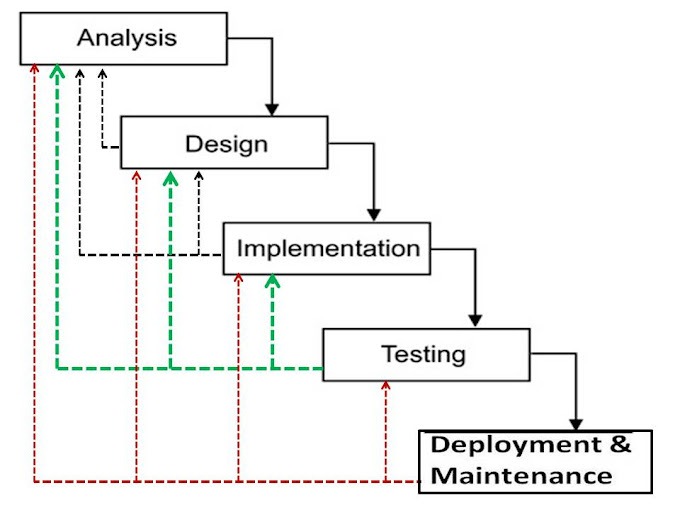
\includegraphics[width=0.6\textwidth]{Images/01 Life_cycle.jpg}  
    \caption{Iterative Waterfall Model}
    \label{Iterative Waterfall Model}  % Label for referencing the figure
\end{figure}


\subsection{Dependencies and Milestones} 
\noindent
Key dependencies were identified for successful project progression. For instance, completion of the data preparation phase was critical before proceeding to model development. Milestones were established at the end of each phase to ensure accountability and track progress. The successful completion of the requirement gathering phase marked the first milestone, followed by the data preparation phase, and so on.

\subsection{Scheduling}
\noindent
Effective scheduling is crucial to the success of any project, as it establishes a clear timeline for tasks, milestones, and dependencies. In the context of our project on detecting mental health disorders through social media analysis, a detailed schedule has been developed to guide the project from inception to completion. This schedule includes specific tasks such as requirement gathering, data preprocessing, model implementation, testing, and deployment, each with clearly defined deadlines. The iterative nature of our chosen methodology allows for flexibility within the schedule, enabling adjustments based on testing outcomes and stakeholder feedback. Key milestones, such as the completion of data analysis, model validation, and user acceptance testing, have been identified to monitor progress and ensure timely delivery of the final product. By utilizing project management tools, such as Microsoft Project, we can visualize and track the progress of tasks, manage resources effectively, and maintain open communication among team members, ensuring that the project stays on schedule and meets its objectives. This proactive approach to scheduling enhances our ability to deliver a high-quality solution that aligns with our goals and stakeholder expectations.

% Insert MS Project Plan Image
\begin{figure}[h!]  
    \centering
    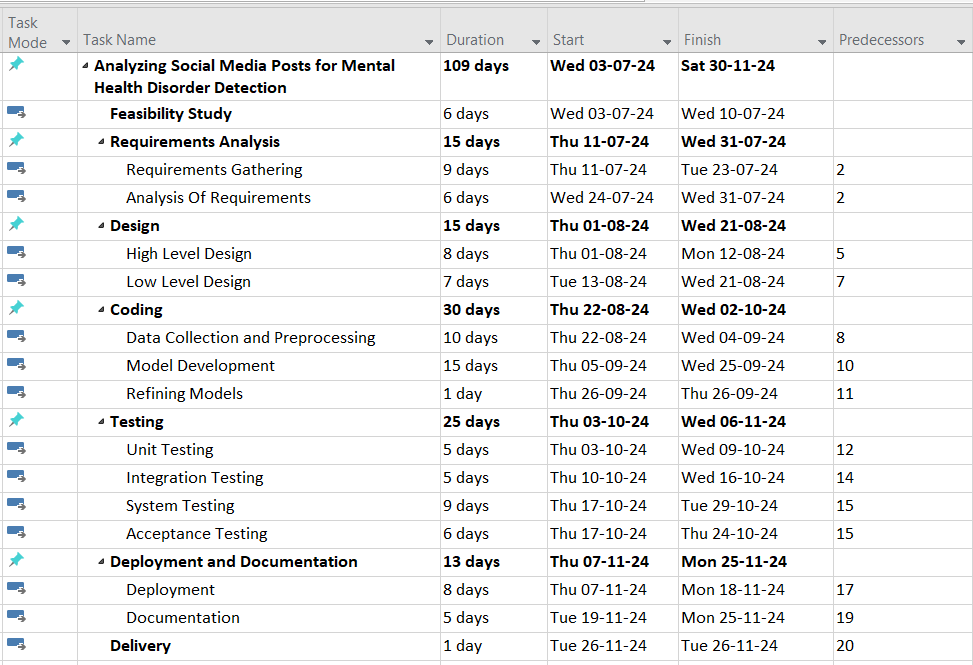
\includegraphics[width=0.9\textwidth]{Images/MS Project Plan Sem 7.png}  
    \caption{Project Plan}
    \label{Project Plan}  % Label for referencing the figure
\end{figure}

\vspace{2cm}

\begin{figure}[h!]  
    \centering
    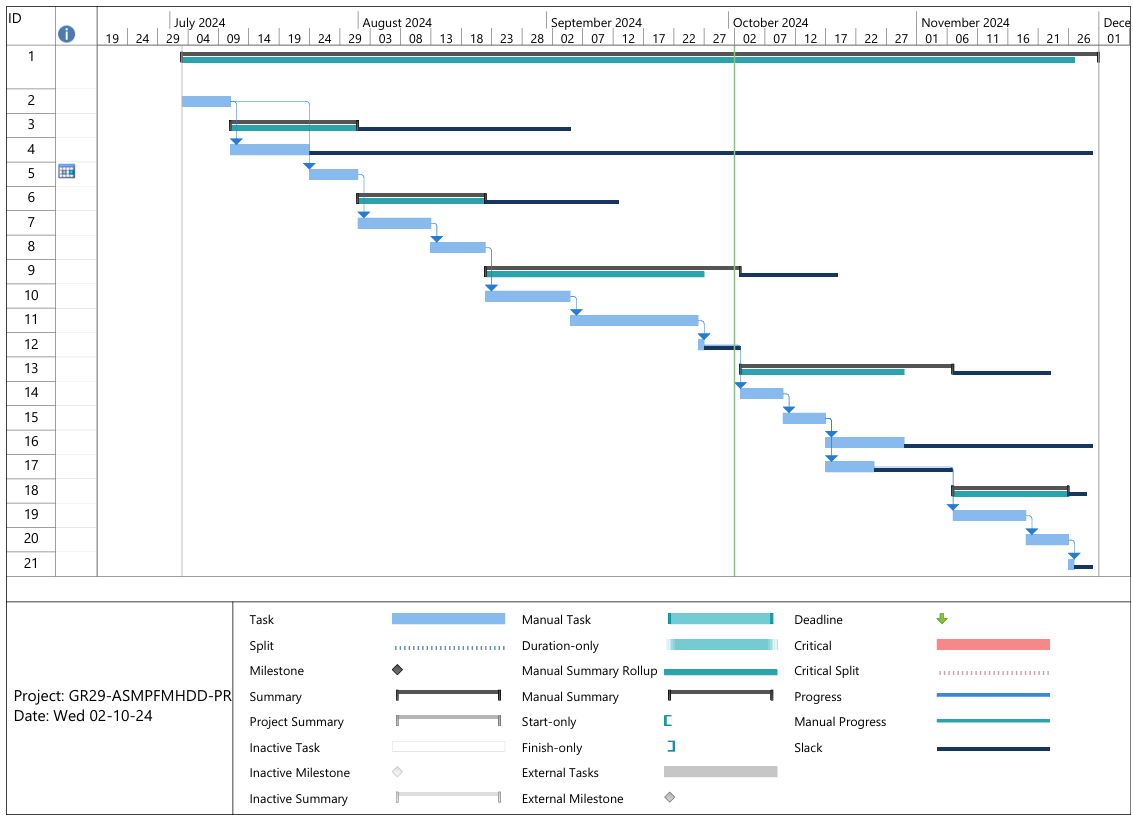
\includegraphics[width=0.9\textwidth]{Images/Gantt Chart.png}  
    \caption{Gantt Chart}
    \label{Gantt Chart}  % Label for referencing the figure
\end{figure}

% ----------------------- Project Planning ends ------------------------------


% --------------------- Requirement Analysis ---------------------------------

\section{Requirement Analysis}

\subsection{Requirement Matrix}
% For Requirement Matrix, latest excel should be pasted and formatted here.
\begin{figure}[h!]  
    \centering
    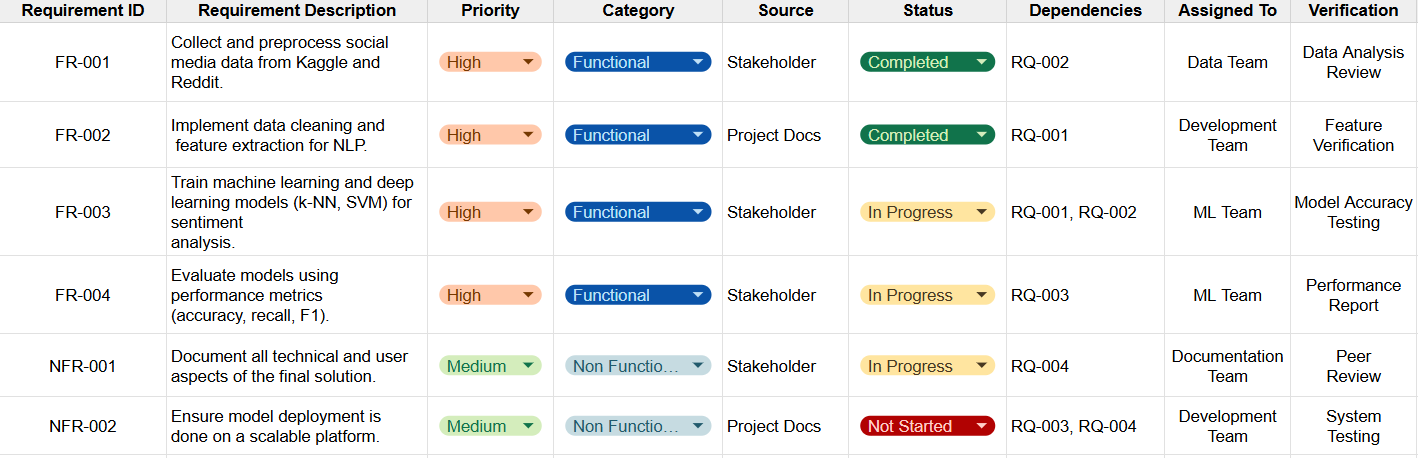
\includegraphics[width=1.0\textwidth]{Images/Requirement Matrix.png}  
    \caption{Requirement Matrix}
    \label{Requirement Matrix}  % Label for referencing the figure
\end{figure}

\noindent
The Requirement Matrix is a comprehensive tool used to track and manage the key requirements of a project. It systematically organizes each requirement with a unique identifier, description, priority, and category (such as functional or non-functional). The matrix also records the source of the requirement, its current status (e.g., in progress, completed), any dependencies on other requirements, and the team or individual responsible for fulfilling it. Additionally, it includes a verification method to ensure the requirement is met, such as through testing or review. This structured format helps ensure that all requirements are clearly defined, prioritized, and tracked, enabling effective project management and ensuring alignment with stakeholder expectations.

\subsection{Requirement Elaboration}
% Create separate sections for separate areas of requirement as in Requirement Matrix. 
% \vspace{.1in}

% \noindent
% For \textbf{Requirement Elaboration}, titles of s6.2.1, 6.2.2 etc. should be with the name of respective requirement areas. Your focus should be on: “What is needed in the system?” Requirement IDs should match with the ID column under Requirement Matrix.

\subsubsection{Functional Requirements}

\noindent
\textbf{\emph{Requirement ID: FR-001}} \\ 
\textbf{\emph{Description: Data Collection}} \\
\textbf{\emph{Priority: High}} \\
\textbf{\emph{Category: Functional}} \\
\noindent
The system requires an ability to collect and ingest a large dataset of Twitter sentiment data from Kaggle. The data should include text content from tweets, associated sentiment labels, and other metadata such as timestamp and user details. This will serve as the primary source of information for sentiment analysis and mental health disorder detection. The system must ensure that the dataset is loaded correctly into the machine learning environment, and any discrepancies in the structure should be handled with pre-processing steps like cleaning, normalization. \\

\noindent
\textbf{\emph{Requirement ID: FR-002}} \\ 
\textbf{\emph{Description: Data Cleaning and Preprocessing}} \\
\textbf{\emph{Priority: High}} \\
\textbf{\emph{Category: Functional}} \\
\noindent
The system must include modules to clean the raw data, such as removing irrelevant characters, handling missing data, and tokenizing text. For the social media posts, it is essential to remove URLs, stopwords, and unnecessary punctuation. The pre-processing pipeline should also convert the text into a suitable numerical format, such as Bag of Words (BoW) or Term Frequency-Inverse Document Frequency (TF-IDF), for further analysis. Proper pre-processing ensures that the data is in a form that can be efficiently used by machine learning models. \\

\noindent
\textbf{\emph{Requirement ID: FR-003}} \\ 
\textbf{\emph{Description: Sentiment and Disorder Detection Model}} \\
\textbf{\emph{Priority: High}} \\
\textbf{\emph{Category: Functional}} \\
\noindent
The system needs to implement machine learning algorithms such as k-Nearest Neighbors (k-NN) and Support Vector Machines (SVM) to classify social media posts based on their sentiment (positive, negative, neutral) and detect potential signs of mental health disorders. The system must be able to train these models on historical data and then apply them to predict the sentiment and detect mental health-related issues in new posts. \\

\noindent
\textbf{\emph{Requirement ID: FR-004}} \\ 
\textbf{\emph{Description: Model Validation and Evaluation}} \\
\textbf{\emph{Priority: High}} \\
\textbf{\emph{Category: Functional}} \\
\noindent
The system must evaluate the performance of the trained models by splitting the dataset into training and test sets. Various performance metrics like accuracy, precision, recall, and F1-score should be computed to assess the model’s effectiveness in detecting mental health disorders. Based on the evaluation, the system should allow for model fine-tuning, such as adjusting hyperparameters, to improve the overall performance. 


\subsubsection{Non Functional Requirements}

\noindent
\textbf{\emph{Requirement ID: NFR-001}} \\ 
\textbf{\emph{Description: Documentation}} \\
\textbf{\emph{Priority: Medium}} \\
\textbf{\emph{Category: Non Functional}} \\
\noindent
The addition of documentation and maintenance manuals as a non-functional requirement ensures that the system is not only usable in the short term but also maintainable and extensible over time. This guarantees that future updates and improvements to the system can be implemented without disrupting existing functionality or requiring a steep learning curve for new developers or users. \\

\noindent
\textbf{\emph{Requirement ID: NFR-002}} \\ 
\textbf{\emph{Description:  Scalability}} \\
\textbf{\emph{Priority: Medium}} \\
\textbf{\emph{Category: Non Functional}} \\
\noindent
The system must be designed to efficiently process large volumes of data, considering the potential growth in the amount of social media posts that need to be analyzed. The data processing pipeline should be scalable to handle increasing data size without significant degradation in performance. This could involve implementing parallel processing techniques or leveraging cloud-based infrastructure to ensure that processing large datasets remains feasible even as the dataset scales. 


% -------------------- Requirement Analysis Ends -----------------------------



% ----------------------------- Design ---------------------------------------

\section{Design}

\subsection{Technical Environment}
% Mention minimum hardware configuration, software tools and package details.
\noindent
The technical environment for the project "Analyzing Social Media Posts for Mental Health Disorder Detection" comprises a combination of hardware, software, and tools that enable smooth data analysis, machine learning model training, and deployment. Below is a detailed overview of the minimum hardware configuration, software tools, and package details necessary to carry out this project effectively. \\

\noindent
\textbf{Minimum Hardware Configuration} \\
\noindent
Given the nature of the project, which involves processing textual data and training machine learning models, the hardware requirements are modest but significant enough to ensure optimal performance. The minimum configuration needed is:
\begin{itemize}
    \item \textbf{Processor} :
    \noindent
    Intel Core i5 (or equivalent) with a base clock speed of at least 2.5 GHz. A multi-core processor is preferred as it helps in parallel processing, which is essential during model training and data preprocessing steps.
    \item \textbf{RAM} :
    \noindent
    8 GB of RAM is recommended to handle the operations of data loading, cleaning, and transformation. Large datasets, like those used in this project, may require more memory to prevent memory overflow errors and reduce delays during processing. For larger datasets, 16 GB of RAM would be ideal.
    \item \textbf{Storage} :
    \noindent
    At least 256 GB of SSD storage is recommended. Faster storage access significantly impacts loading time for datasets and dependencies. SSD is preferred over traditional HDD because of its faster read/write speeds, which benefit large datasets like the Reddit-based social media posts used in this project.
    \item \textbf{Graphics Processing Unit (GPU)} :
    \noindent
    For basic machine learning tasks like Logistic Regression or SVM, a dedicated GPU is not necessary. However, if deep learning models or more complex neural networks were introduced later, a GPU like NVIDIA GTX 1060 with 4 GB VRAM or higher would be advantageous.
    \item \textbf{Operating System} :
    \noindent
    Windows 10 (64-bit) or higher, macOS 10.13 (High Sierra) or higher, or any stable Linux distribution (e.g., Ubuntu 18.04 or higher). The operating system should support all necessary machine learning libraries and be compatible with the tools required for the project.
\end{itemize} \\

\noindent
\textbf{Software Tools and Packages} \\
\noindent
For the software stack, the project leverages a set of well-established tools, platforms, and programming libraries to ensure smooth execution from data preprocessing to model deployment:
\begin{itemize}
    \item \textbf{Python} :
    \noindent
    The primary programming language used for data processing, model training, and evaluation. Python is chosen due to its rich ecosystem of libraries and frameworks tailored for machine learning and data science.
    \item \textbf{Google Colab} :
    \noindent
    A cloud-based platform used for writing, executing, and sharing Python code. Google Colab provides free access to GPU and TPU resources, which is beneficial for intensive model training tasks. It also offers seamless integration with libraries like TensorFlow and PyTorch.
    \item \textbf{Jupyter Notebooks} :
    \noindent
     An alternative environment for running Python code, offering an interactive interface to write and execute code in blocks. It allows for easy visualization of results and is highly suitable for collaborative projects.
\end{itemize}

\pagebreak

\noindent
\textbf{Python Packages and Libraries}
\begin{table}[h!]
\centering
\begin{tabular}{|p{9cm}|p{6cm}|}
  \hline
  \multicolumn{1}{|c|}{\textbf{Package}} & \multicolumn{1}{c|}{\textbf{Purpose}} \\
  
  \hline
  \texttt{praw} & Access Reddit posts for data collection. \\
  
  \hline
  \texttt{pandas} & Data manipulation and analysis. \\
  
  \hline
  \texttt{textblob} & Text processing and sentiment analysis. \\
  
  \hline
  \texttt{time} & Managing execution time. \\
  
  \hline
  \texttt{re} & Regular expressions for text cleaning. \\
  
  \hline
  \texttt{TfidfVectorizer} & Convert text to TF-IDF features. \\
  
  \hline
  \texttt{stopwords} & Remove stopwords from text. \\
  
  \hline
  \texttt{tokenize} & Tokenize text data. \\
  
  \hline
  \texttt{nltk} & Natural Language Toolkit for text processing. \\
  
  \hline
  \texttt{CountVectorizer} & Convert text to Bag-of-Words features. \\
  
  \hline
  \texttt{split} & Split the dataset into training and testing sets. \\
  
  \hline
  \texttt{LogisticRegression} & Build and train Logistic Regression models. \\
  
  \hline
  \texttt{sklearn.metrics.accuracy\_score} & Calculate accuracy of the model. \\
  
  \hline
  \texttt{report} & Generate classification performance report. \\
  
  \hline
  \texttt{RandomizedSearchCV} & Hyperparameter tuning for models. \\
  
  \hline
  \texttt{seaborn} & Data visualization and plotting. \\
  
  \hline
  \texttt{matplotlib.pyplot} & Create and customize plots. \\
  
  \hline
  \texttt{matrix} & Generate confusion matrix. \\
  
  \hline
  \texttt{roc\_curve, auc, roc\_auc\_score} & Evaluate model’s ROC and AUC scores. \\
  
  \hline
  \texttt{KNeighborsClassifier} & Build k-Nearest Neighbors (k-NN) models. \\
  
  \hline
  \texttt{svm.SVC} & Build Support Vector Machines (SVM) models. \\
  
  \hline
  \texttt{naive\_bayes.MultinomialNB} & Build Naive Bayes models. \\
  
  \hline
  \texttt{scipy.stats.uniform} & Statistical operations for tuning models. \\
  
  \hline
  \texttt{RandomForestClassifier} & Build Random Forest models. \\
  
  \hline
  \texttt{sklearn.preprocessing.label\_binarize} & Convert labels for multi-class ROC analysis. \\
  
  \hline
\end{tabular}
\end{table}



\pagebreak

\subsection{Hierarchy of Modules}
% Provide a diagram.
\begin{figure}[h!]  
    \centering
    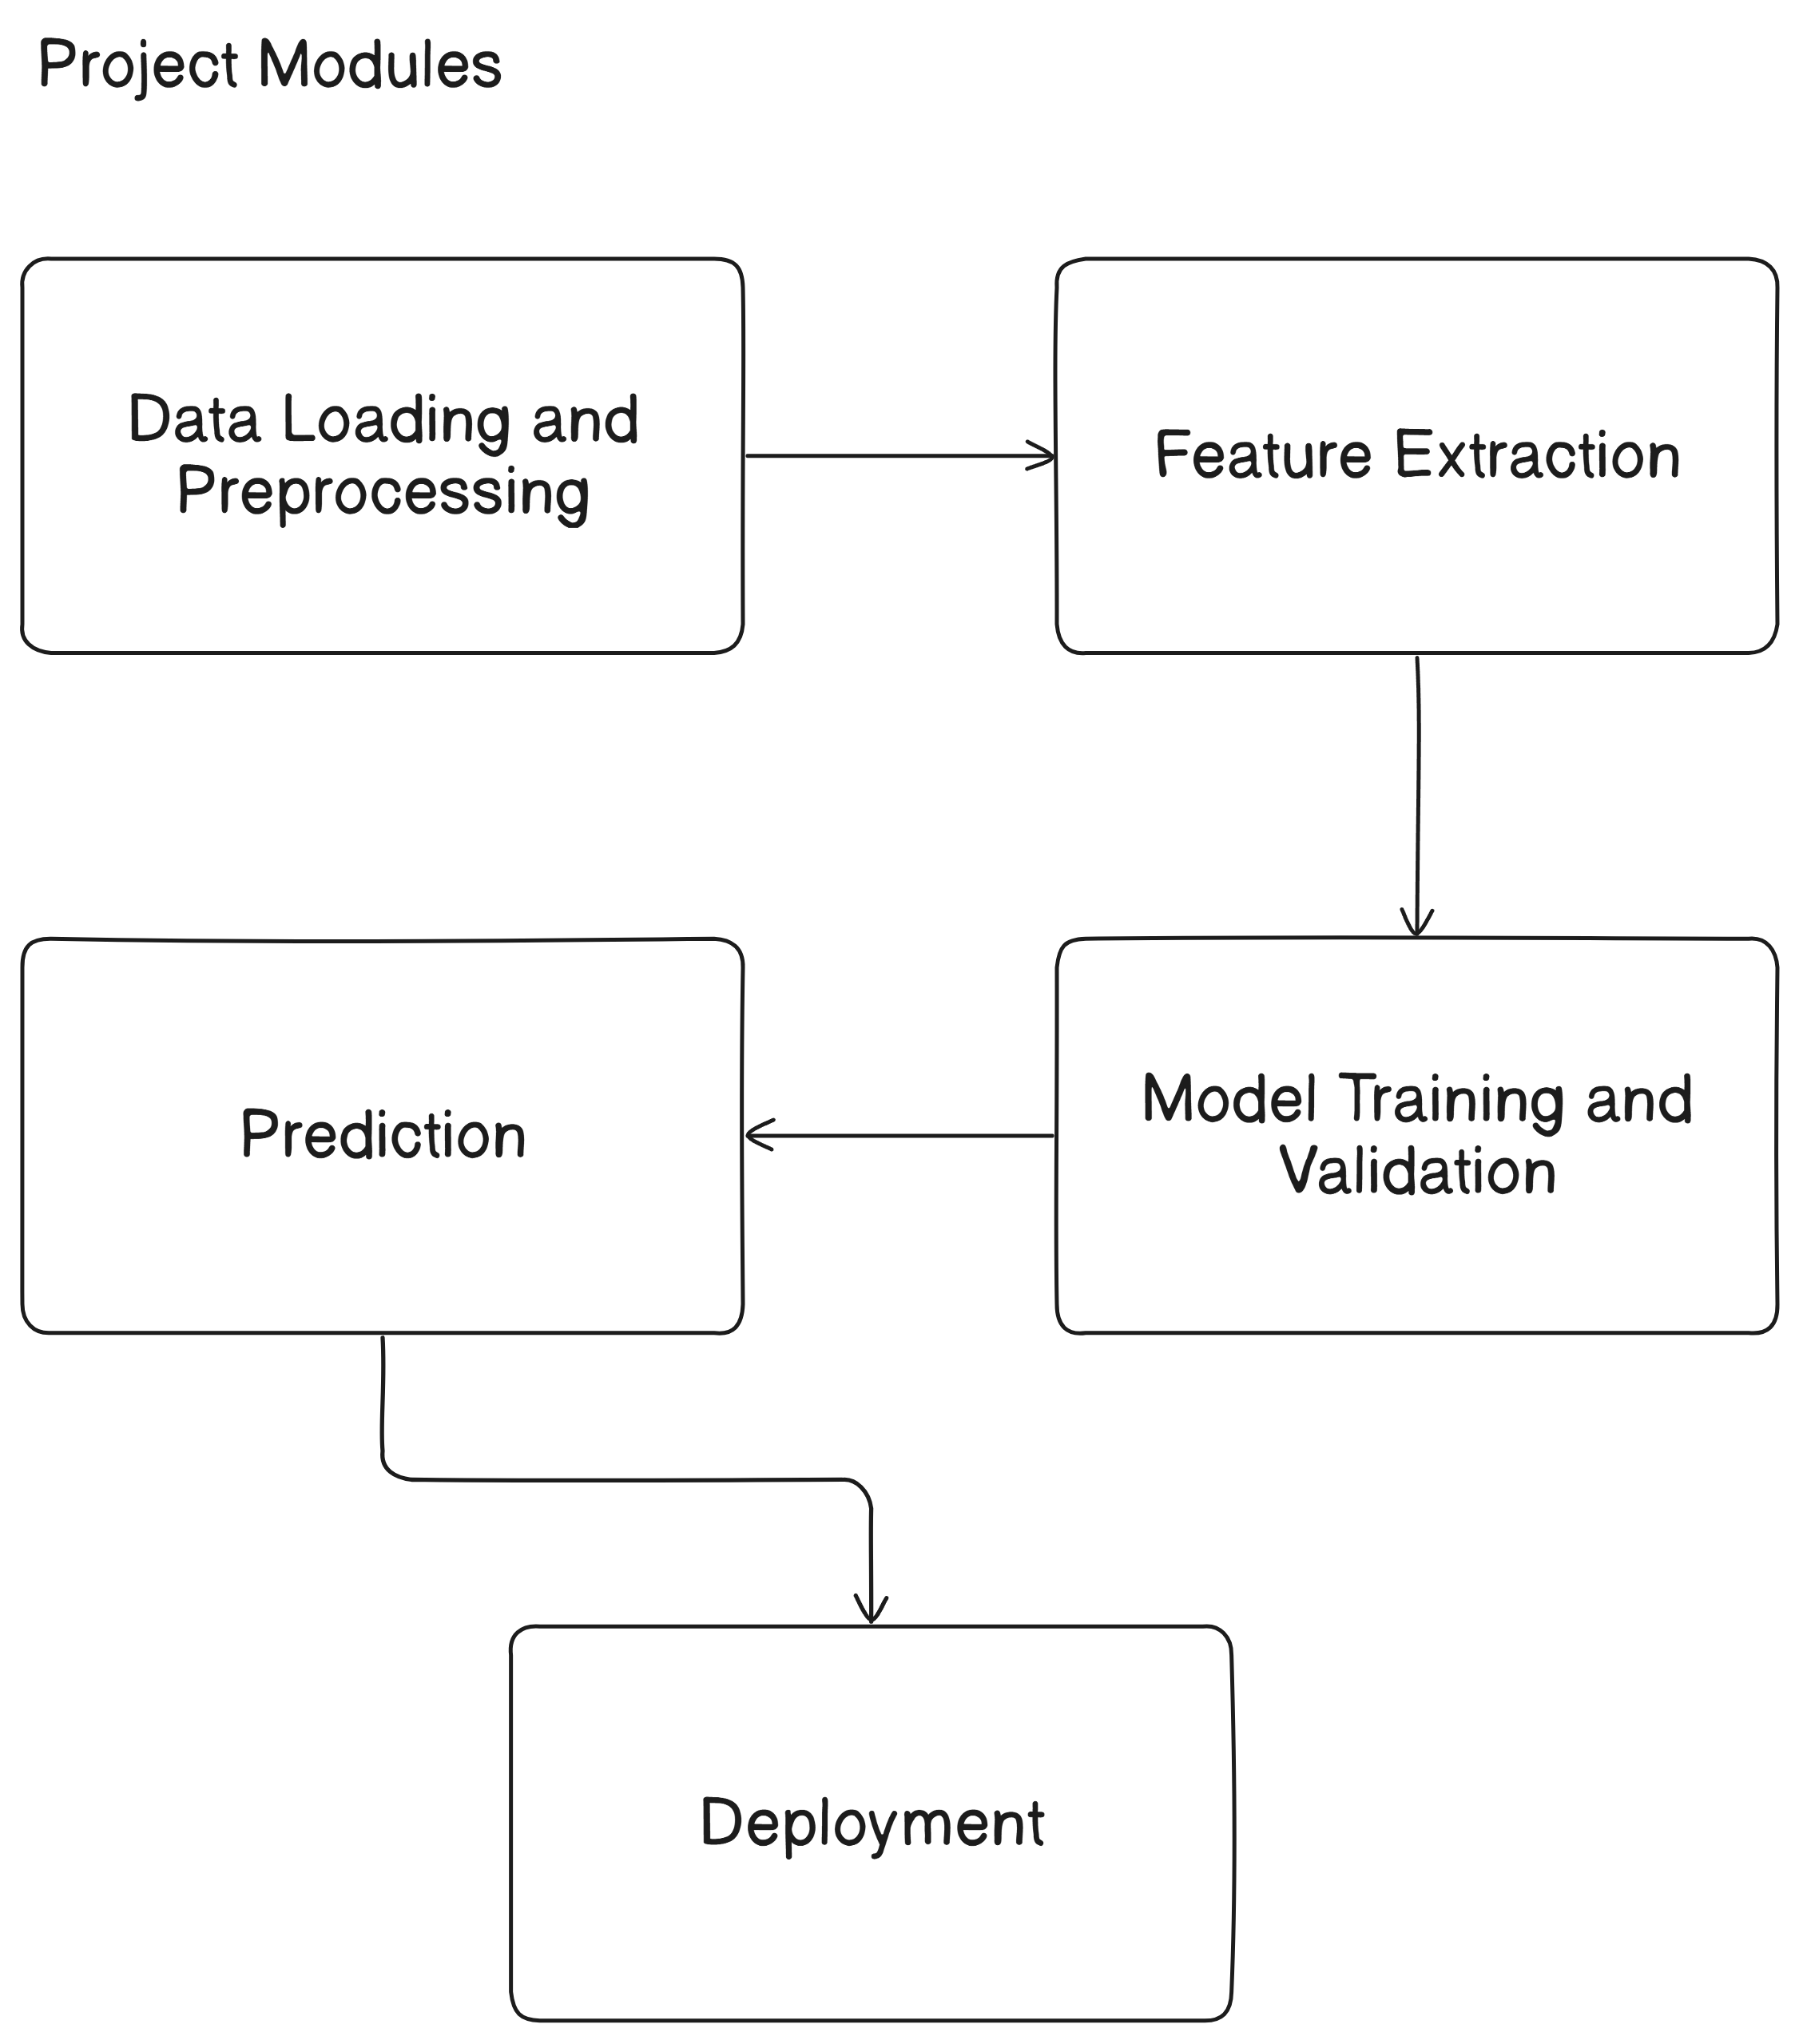
\includegraphics[width=0.6\textwidth]{Images/Project Modules.png}  
    \caption{Project Modules}
    \label{Project Modules}  % Label for referencing the figure
\end{figure}

\noindent
In this project, the system is organized into several key modules to efficiently classify mental health issues based on text input. The Data Loading and Preprocessing Module is responsible for loading the CSV data from preprocessed\_mental\_health\_text.csv and performing essential text cleaning operations, such as tokenization and stop-word removal, to prepare the data for analysis. Following this, the Feature Extraction Module employs techniques like Bag of Words or TF-IDF to convert the cleaned text into numerical features suitable for classification. The Model Training and Validation Module takes these features, splitting the dataset into training and testing sets, and implements multiple machine learning models, including Logistic Regression, k-Nearest Neighbors (k-NN), Support Vector Machines (SVM), Naive Bayes, and Random Forest. Each model is evaluated using relevant metrics to assess accuracy and performance. The Prediction Module is designed to accept new input text and utilize the trained models to predict mental health issues, ensuring that various perspectives from the different algorithms are considered. Finally, the Deployment Module offers a free solution for serving the models, potentially utilizing platforms like Google Colab or Hugging Face, allowing for real-time predictions in practical applications.

\subsection{Detailed Design}
% Provide hierarchy of modules or overall system diagram. 
% \vspace{.1in}
\begin{figure}[h!]  
    \centering
    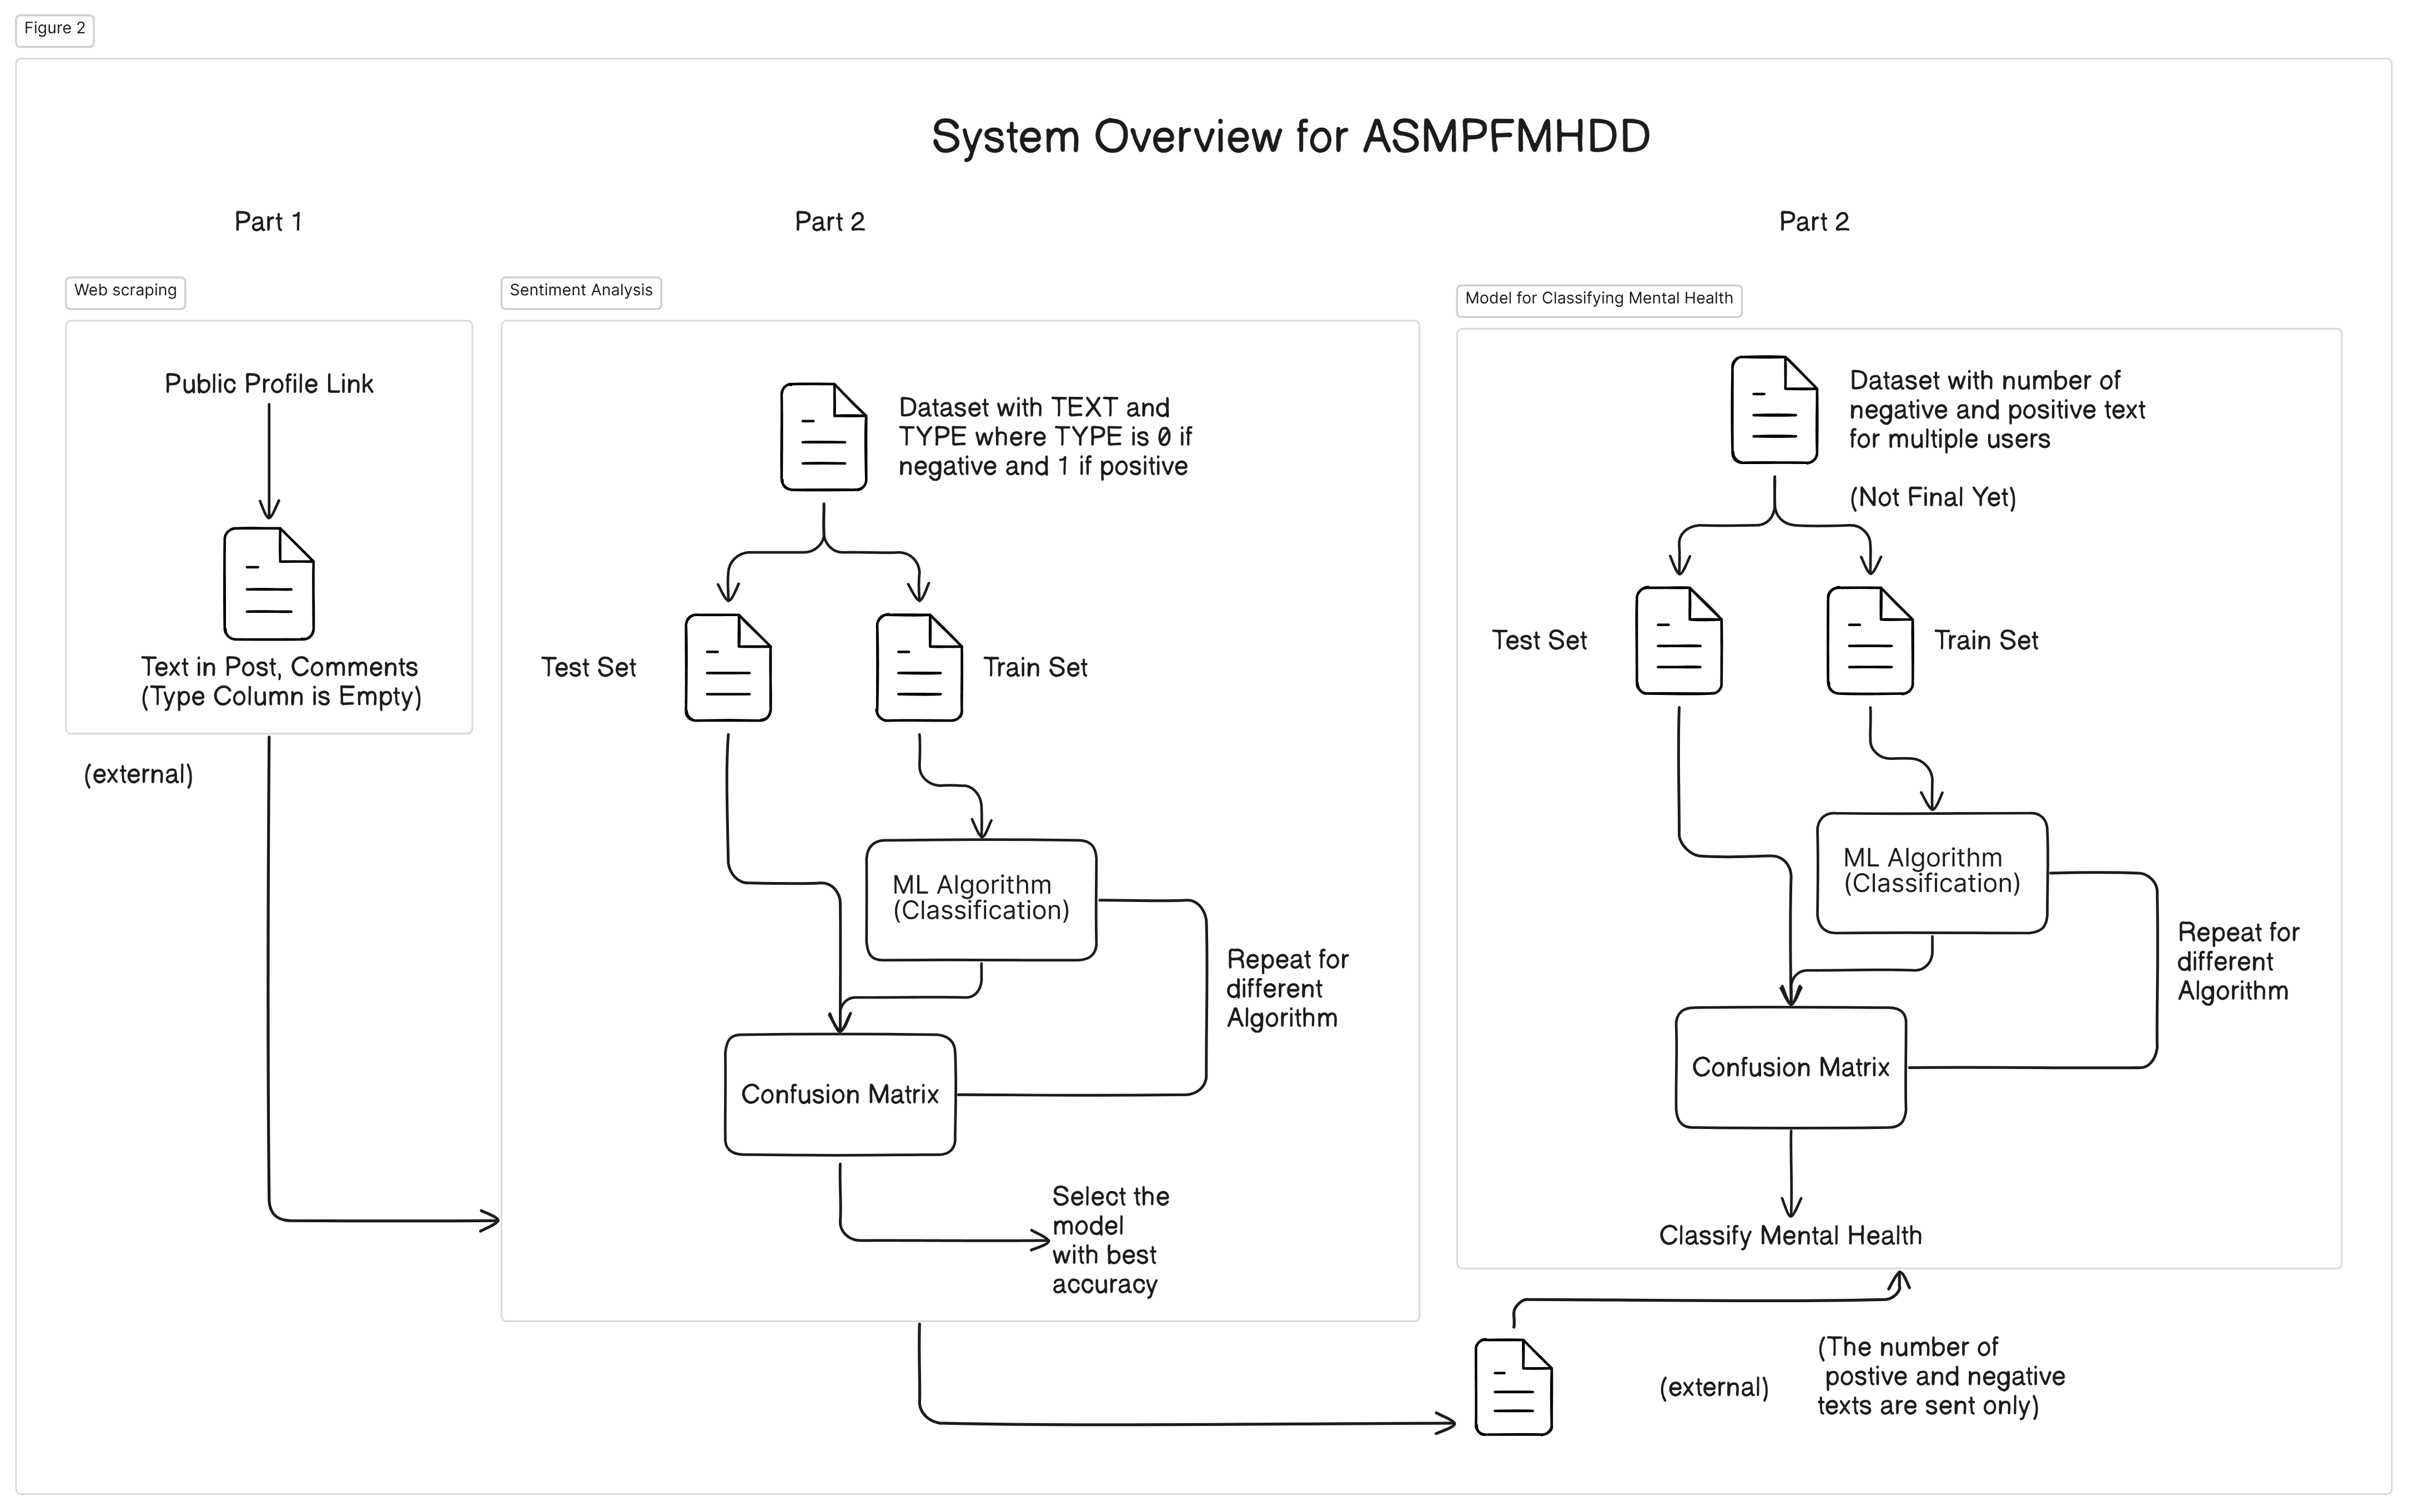
\includegraphics[width=1.0\textwidth]{Images/System Overview.png}  
    \caption{System Overview}
    \label{System Overview}  % Label for referencing the figure
\end{figure}

\begin{figure}[h!]  
    \centering
    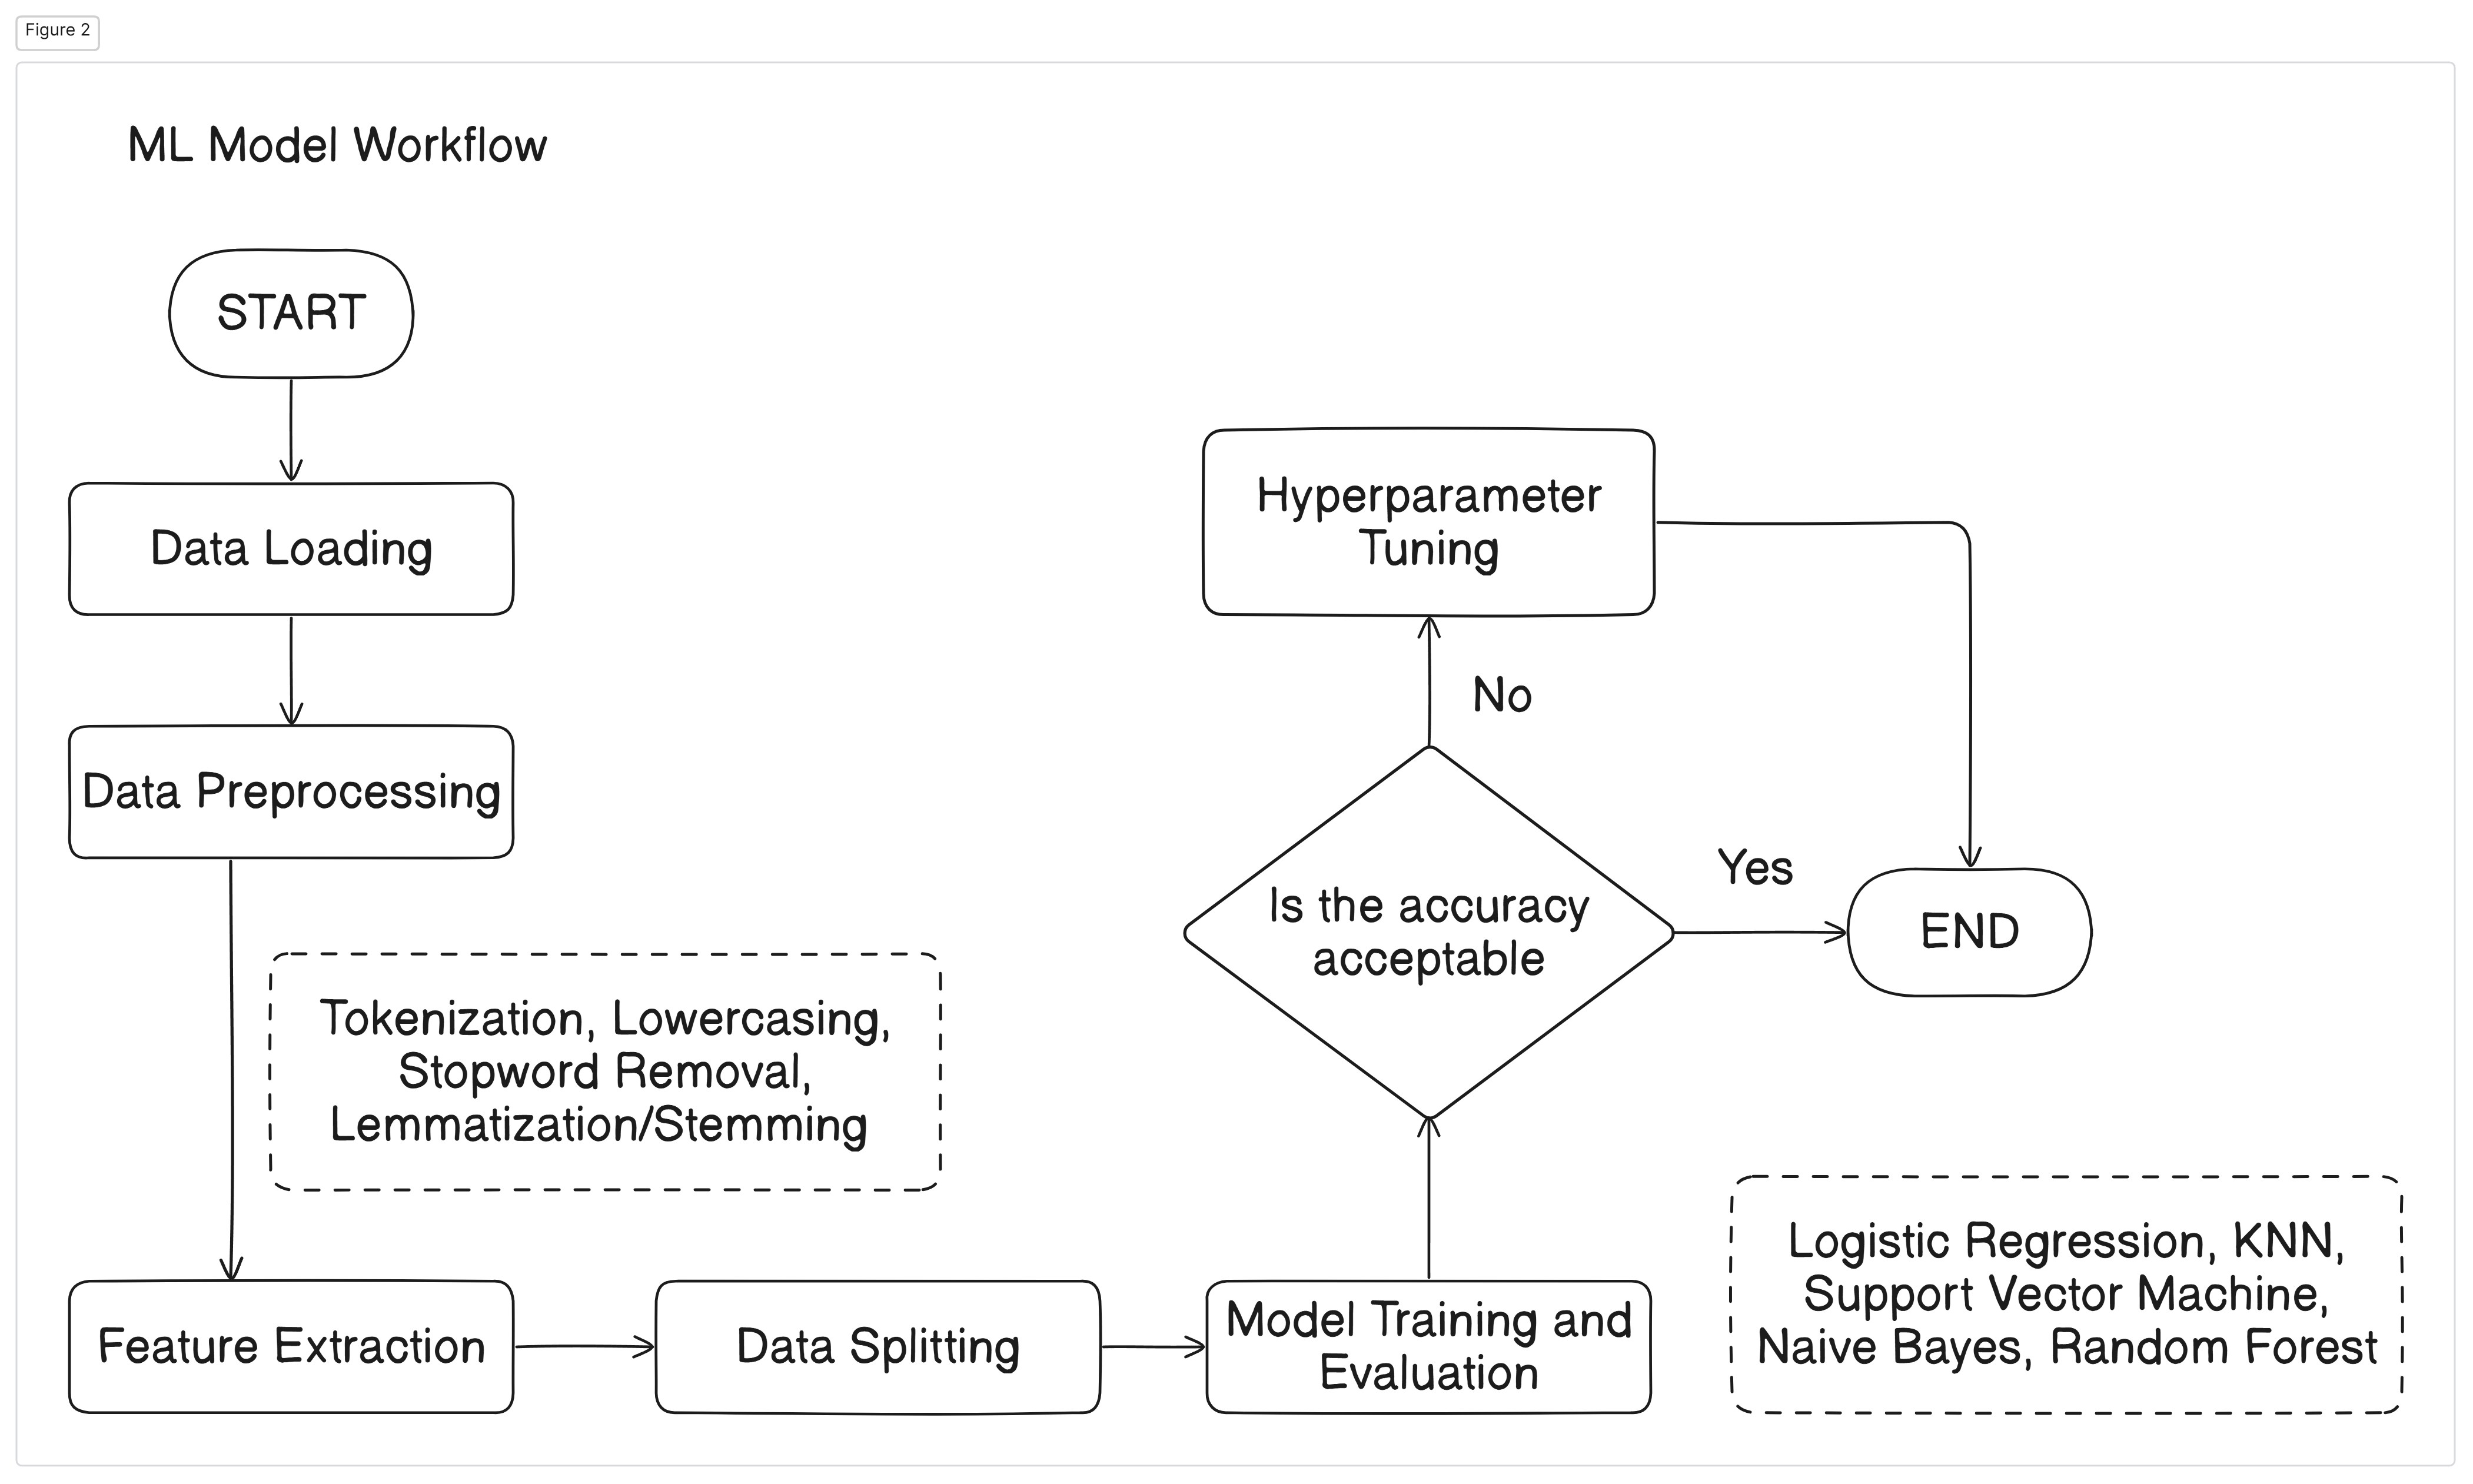
\includegraphics[width=0.95\textwidth]{Images/ML Model Workflow.png}  
    \caption{Model Workflow}
    \label{Model Workflow}  % Label for referencing the figure
\end{figure}

% \noindent
% For Detailed Design, use flowcharts, DFD, UML or ER diagrams as applicable. Titles of s7.2.1, 7.2.2 etc. should be with the name of respective design modules. Your focus should be on: “How the requirement will be implemented in the system?” Design Reference subsection numbers should be matching as stated in Requirement Matrix.
\vspace{.1in}

\subsubsection{Data Loading and Preprocessing}
\noindent
The Data Loading and Preprocessing Module is the foundation of the system, responsible for ingesting and preparing the text data for analysis. This module begins by loading the dataset from the preprocessed\_mental\_health\_text.csv file, which contains various mental health-related text entries. Once the data is loaded, a series of preprocessing steps are conducted to ensure the text is clean and ready for feature extraction. This includes tokenization, where the text is split into individual words or tokens, and lowercasing to maintain uniformity across the dataset. Additionally, stop-word removal is performed to eliminate common words that do not contribute to the meaning, such as "and," "the," and "is." Finally, lemmatization or stemming is applied to reduce words to their base or root forms. These preprocessing techniques are crucial as they help improve the quality of the input data, ultimately leading to better model performance.

\subsubsection{Feature Extraction}
\noindent
In the Feature Extraction Module, the preprocessed text data is transformed into a numerical format that machine learning algorithms can process. This module allows for the selection between two primary feature extraction methods: Bag of Words (BoW) and Term Frequency-Inverse Document Frequency (TF-IDF). The Bag of Words model creates a representation of the text based on the frequency of words, disregarding the order in which they appear, which simplifies the input for classification algorithms. Alternatively, the TF-IDF approach evaluates the importance of words in the dataset by considering their frequency in individual documents relative to their overall occurrence across all documents. This helps in highlighting the most informative words. By converting text into numerical features, this module prepares the data for the subsequent training and validation stages, ensuring that the classification models can effectively interpret the input.

\subsubsection{Model Training and Validation}
\noindent
The Model Training and Validation Module is critical to developing a robust classification system. In this module, the dataset is split into training and testing sets to evaluate the performance of the models accurately. Various classification algorithms are employed, including Logistic Regression, k-Nearest Neighbors (k-NN), Support Vector Machines (SVM), Naive Bayes, and Random Forest. Each model is trained on the training set, which involves adjusting the model parameters based on the input features and their corresponding labels. Following training, the models undergo validation to assess their performance using various metrics such as accuracy, precision, recall, and F1-score. A decision point is included to determine if the achieved accuracy meets the project requirements. If the accuracy is deemed acceptable, the model proceeds to the deployment stage. 

\begin{figure}[h!]  
    \centering
    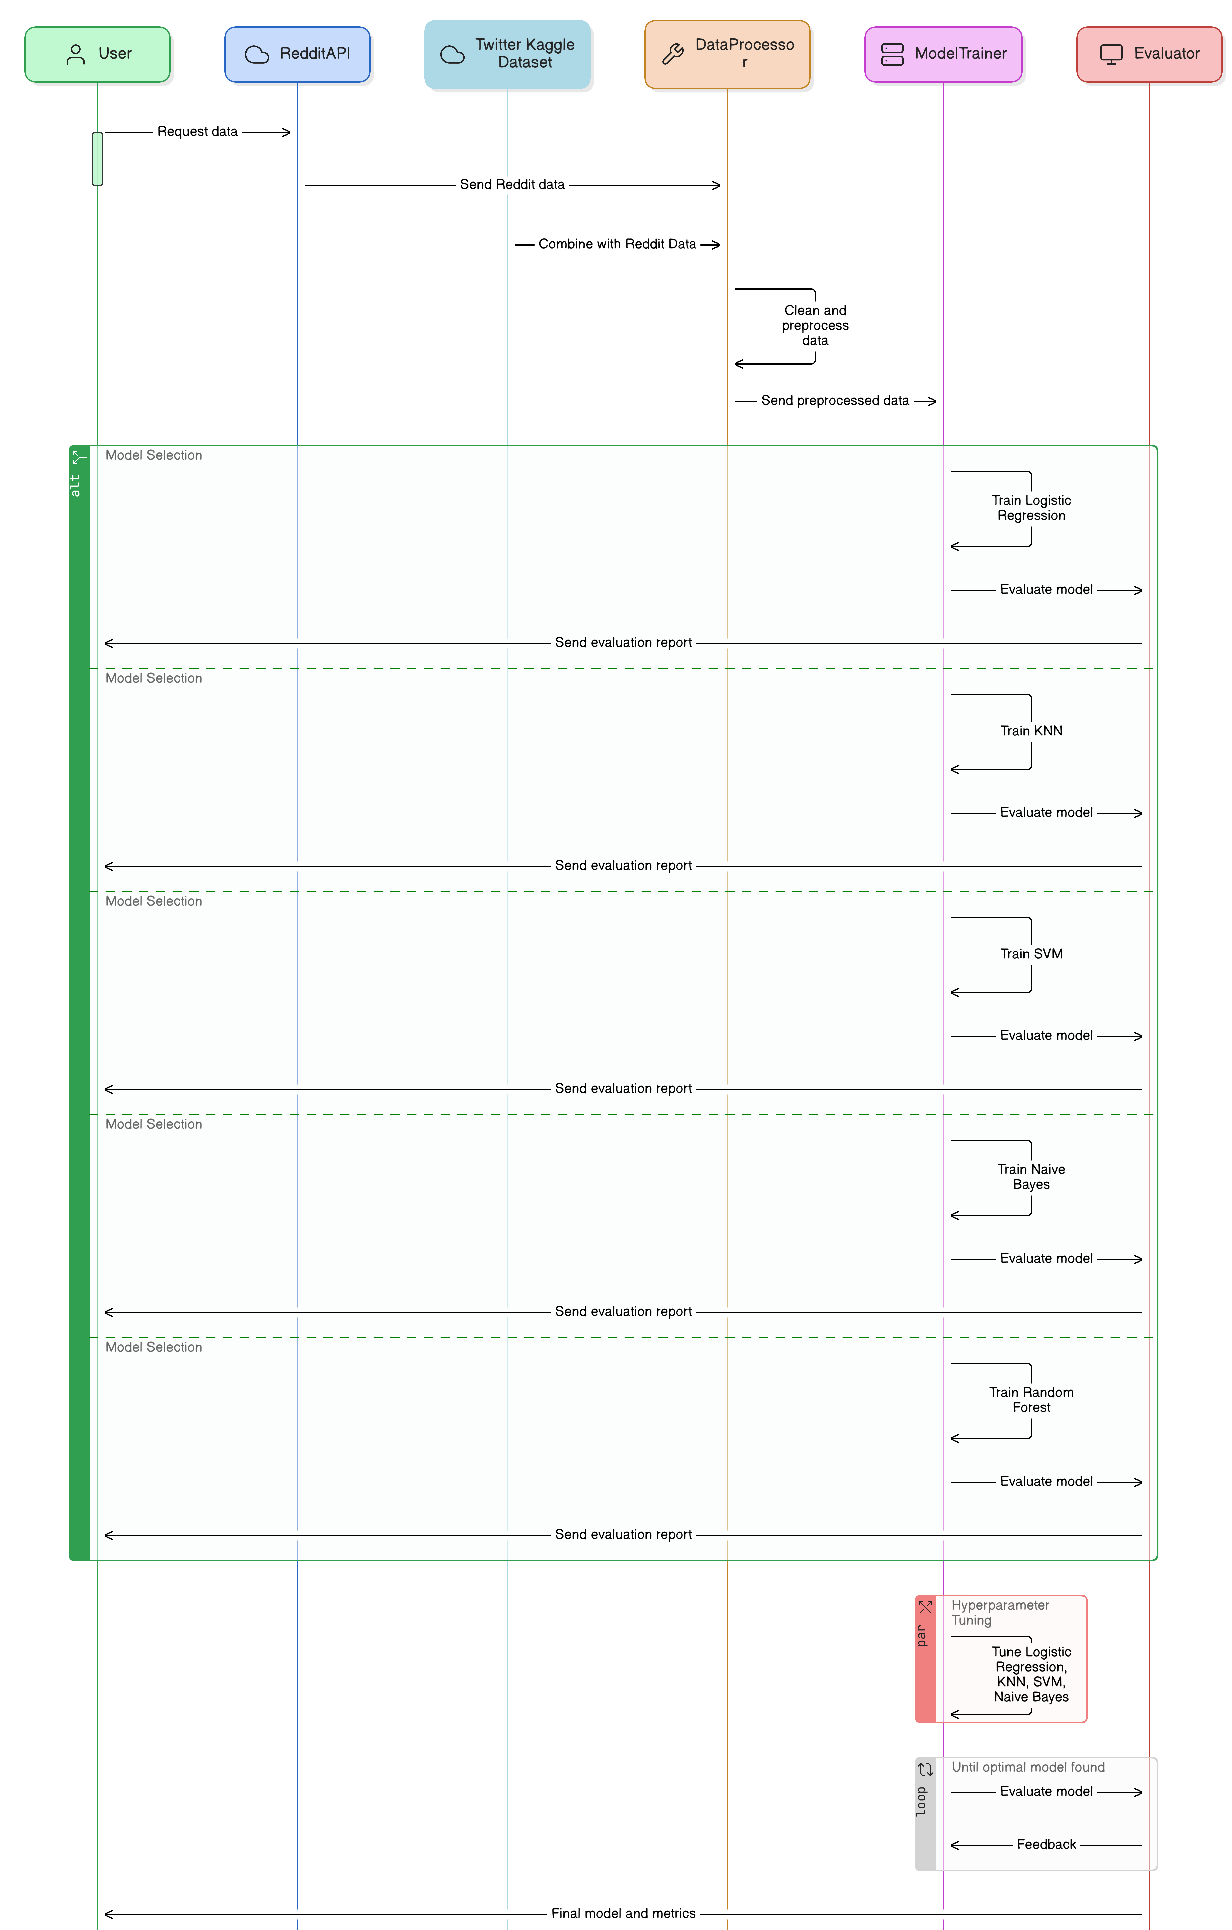
\includegraphics[width=0.85\textwidth]{Images/Project Sequence.png}  
    \caption{Project Sequence}
    \label{Project Sequence}  % Label for referencing the figure
\end{figure}

\subsubsection{Prediction}
\noindent
The Prediction Module is designed to provide real-time classification of new input text related to mental health issues. Upon receiving user input, this module initiates a preprocessing workflow that mirrors the steps applied during the training phase, including tokenization, lowercasing, stop-word removal, and lemmatization or stemming. Once the input text is preprocessed, it is fed into the trained classification models to generate predictions. Each model may provide a classification result, allowing for a comprehensive analysis of the input. This module not only delivers the predicted mental health issue but also ensures that users receive an informative output that reflects the confidence level of each prediction, enabling them to understand the model's reasoning. The seamless integration of this module into the overall system enhances the user experience by providing instant and relevant feedback.

\subsubsection{Deployment}
\noindent
The Deployment Module focuses on making the trained models accessible for real-time predictions. Once the models have been validated and selected based on their performance, this module prepares them for deployment on suitable platforms, such as Google Colab or Hugging Face. This involves packaging the models and creating a user interface where users can input text and receive predictions. The deployment process also includes considerations for scaling, ensuring that the system can handle multiple requests simultaneously while maintaining responsiveness. By providing a free and efficient deployment solution, this module enables users to access the mental health classification service easily. The deployment of the models ensures that the insights generated from the analysis can be utilized effectively in real-world applications, contributing to better mental health awareness and support.

% \noindent
% Create separate sections for separate modules of design as in Requirement Matrix. Ensure to provide Design Diagrams \textit{(e.g. System overview / DFDs / ERDs etc.; cross-reference to be drawn from Chapter 6), Decision matrix (for algorithm recommendation etc.) }




% \subsubsection{Name of Design Module 1 \label{sec:design_mod1}}
% \subsubsection{Name of Design Module 2 \label{sec:design_mod2}}
% \subsubsection{Name of Design Module 3 etc \label{sec:design_mod3}}


% Refer APPENDIX A  – Prototypes \ref{sec:proto} for prototype details.


% ------------------------------ Design Ends ---------------------------------


% --------------------------- Implementation ---------------------------------

\section{Implementation}
%Focus of 7\textsuperscript{th} semester deliverables are analysis, design and prototyping. Refer APPENDIX A – Prototypes for prototype details.
% For Test Planning, s6.4 should contain the Test Plan in tabular format, where each Test
% Case should be represented with distinct id, prefixed with ``T-$<<$module$>>$-'', where module represents the short code of the respective design module. 
% Test Case numbers should be matching as stated in Requirement Matrix.

\subsection{Features From RM}
\noindent
For the initial prototype development, a subset of the requirements from the Requirement Matrix (RM) was carefully selected to focus on implementing core functionalities and demonstrating proof of concept. The selection was based on a combination of high-priority functional requirements that form the backbone of the system, ensuring that critical features are built and validated before expanding the scope.

The requirements chosen for the prototype primarily involve data preprocessing, model training, and evaluation processes. These requirements were selected because they are fundamental to the project's success, ensuring that the data pipeline and model implementation work seamlessly together. This subset of features lays the groundwork for later integration with additional components and more complex functionality.

The filtered part of the RM focuses on the following high-priority requirements: data cleaning and feature extraction, training of machine learning models, and evaluation of model performance using standard metrics. These requirements were identified as crucial because they directly impact the system's ability to handle data, learn patterns, and provide meaningful outputs. Without successfully implementing these core features, the overall effectiveness of the solution would be significantly reduced.

Furthermore, these selected features align with the project’s goals and provide a clear pathway for incremental development. By narrowing down the requirements to these foundational aspects, the development team can ensure that the prototype is not only functional but also extensible, providing a robust framework for future enhancements.

\begin{figure}[h!]  
    \centering
    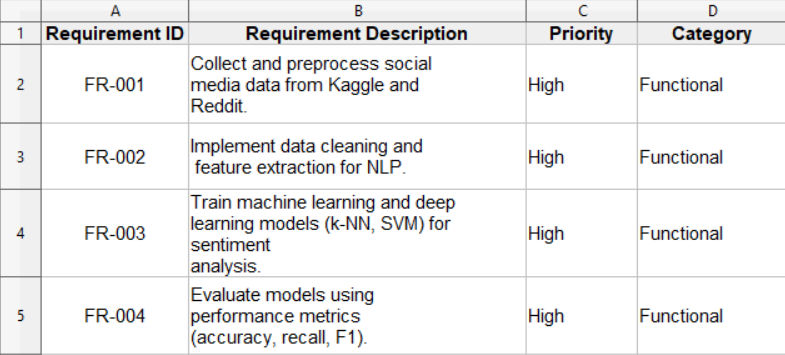
\includegraphics[width=0.85\textwidth]{Images/RM_part_for_implementation.png}  
    \caption{Features from Requirement Matrix}
    \label{Features from Requirement Matrix}  % Label for referencing the figure
\end{figure}

\subsection{Steps of Compilation, Execution and Setup}
\begin{enumerate}
    \item \textbf{Setup the Development Environment}
    \begin{itemize}
        \item Ensure Python 3.x is installed on your system.
        \item Install a virtual environment package if not already available:
        \begin{verbatim}
        pip install virtualenv
        \end{verbatim}
        \item Create a virtual environment for the project:
        \begin{verbatim}
        python -m venv project_env
        \end{verbatim}
        \item Activate the virtual environment:
        \begin{itemize}
            \item For Windows:
            \begin{verbatim}
            .\project_env\Scripts\activate
            \end{verbatim}
            \item For Linux/Mac:
            \begin{verbatim}
            source project_env/bin/activate
            \end{verbatim}
        \end{itemize}
    \end{itemize}

    \item \textbf{Install Required Libraries}
    \begin{itemize}
        \item Install the necessary Python libraries using the following command:
        \begin{verbatim}
        pip install pandas numpy scikit-learn matplotlib
        \end{verbatim}
        \item If your project has additional dependencies, include them as well:
        \begin{verbatim}
        pip install tensorflow keras seaborn
        \end{verbatim}
    \end{itemize}

    \item \textbf{Set Up the Project Directory}
    \begin{itemize}
        \item Organize your project directory as follows:
        \begin{verbatim}
        project_folder/
        ├── data/
        │   └── sample_data.csv
        ├── notebooks/
        │   └── project_prototype.ipynb
        ├── src/
        │   └── main.py
        └── requirements.txt
        \end{verbatim}
        \item Place your input data files in the \texttt{data/} folder.
        \item Store Jupyter notebooks in the \texttt{notebooks/} folder.
        \item Add the main code files in the \texttt{src/} folder.
    \end{itemize}

    \item \textbf{Configure the Jupyter Notebook Environment}
    \begin{itemize}
        \item Navigate to the \texttt{notebooks/} folder using the command line:
        \begin{verbatim}
        cd notebooks
        \end{verbatim}
        \item Launch Jupyter Notebook:
        \begin{verbatim}
        jupyter notebook
        \end{verbatim}
        \item Open the \texttt{project\_prototype.ipynb} file from the Jupyter interface and execute each cell sequentially to run the prototype.
    \end{itemize}

    \item \textbf{Compilation and Execution of the Main Code (If Using Scripts)}
    \begin{itemize}
        \item If you are running the project using a script (e.g., \texttt{main.py}), navigate to the \texttt{src/} folder:
        \begin{verbatim}
        cd ../src
        \end{verbatim}
        \item Run the main script:
        \begin{verbatim}
        python main.py
        \end{verbatim}
        \item Ensure that the paths to the data files and other dependencies are correctly set in your code.
    \end{itemize}

    \item \textbf{Setup Test Data for Evaluation}
    \begin{itemize}
        \item Place the test dataset in the \texttt{data/} folder, ensuring it follows the format specified in the documentation.
        \item If using the command line, you can test with different data files by updating the file path in the code or using command-line arguments.
    \end{itemize}

    \item \textbf{View and Analyze the Output}
    \begin{itemize}
        \item For Jupyter Notebooks, observe the outputs directly in the notebook cells.
        \item If using scripts, the results (e.g., model performance, accuracy metrics, or visualizations) will be printed to the console or saved as files in the \texttt{output/} folder, depending on the implementation.
    \end{itemize}

    \item \textbf{Document and Verify the Execution}
    \begin{itemize}
        \item Document any issues or errors encountered during the compilation and execution.
        \item Perform a verification of results against the expected outputs to ensure correctness.
    \end{itemize}
\end{enumerate}

\subsection{Code Details and Output}

% Data Collection
\subsubsection{Data Collection: Scraping Reddit Posts}
\noindent
The code snippet below demonstrates how Reddit posts related to mental health issues are collected and preprocessed for further analysis. This process involves using the `praw` library to access the Reddit API, collecting posts from specified subreddits, extracting text data, calculating sentiment scores using `TextBlob`, and saving the processed data into a CSV file.

\begin{itemize}
    \item \textbf{Library Installation and Importation:}
    \begin{verbatim}
    !pip install praw
    import praw
    import pandas as pd
    from textblob import TextBlob
    import time
    \end{verbatim}
    \noindent
    The code starts by installing and importing necessary libraries: 
    \texttt{praw} (Python Reddit API Wrapper) for accessing Reddit data, 
    \texttt{pandas} for handling tabular data, 
    \texttt{TextBlob} for sentiment analysis, 
    and \texttt{time} for managing pauses during the scraping process to avoid rate limits.

    \item \textbf{Reddit API Authentication:}
    \begin{verbatim}
    reddit = praw.Reddit(client_id=<Reddit Client ID>,
                         client_secret=<Reddit Client Secret>,
                         user_agent='Mental Health')
    \end{verbatim}
    \noindent
    Here, the Reddit API credentials (`client\_id`, `client\_secret`, and `user\_agent`) are specified to create an authorized `praw.Reddit` object, which will be used to interact with Reddit.

    \item \textbf{Defining Subreddits to Scrape:}
    \begin{verbatim}
    subreddits = ['normal','depression','anxiety','bipolar','ptsd']
    \end{verbatim}
    \noindent
    The subreddits related to mental health are stored in a list named `subreddits`. These communities are targeted for data collection.

    \item \textbf{Setting Up Post Collection:}
    \begin{verbatim}
    post_types = ['hot', 'new', 'top']
    posts_per_type = 1500
    \end{verbatim}
    \noindent
    Three categories of posts are selected: `hot`, `new`, and `top`. The number of posts to be collected from each category is set to 1500.

    \item \textbf{Iterating through Subreddits and Post Types:}
    \begin{verbatim}
    for subreddit in subreddits:
        for post_type in post_types:
            if post_type == 'hot':
                subreddit_posts = reddit.subreddit(subreddit).
                hot(limit=posts_per_type)
            elif post_type == 'new':
                subreddit_posts = reddit.subreddit(subreddit).
                new(limit=posts_per_type)
            elif post_type == 'top':
                subreddit_posts = reddit.subreddit(subreddit).
                top(limit=posts_per_type)
    \end{verbatim}
    \noindent
    Nested loops are used to iterate through each subreddit and post type, creating a collection of posts from each combination.

    \item \textbf{Collecting and Labeling Data:}
    \begin{verbatim}
    for post in subreddit_posts:
        post_content = post.title + " " + post.selftext
        sentiment = TextBlob(post_content).sentiment.polarity
    \end{verbatim}
    \noindent
    Each post’s title and content are concatenated into a single string. Sentiment analysis is then performed using `TextBlob` to generate a polarity score, which ranges from -1 (negative) to 1 (positive).

    \item \textbf{Assigning Sentiment Labels:}
    \begin{verbatim}
    if sentiment > 0:
        sentiment_label = 1.0
    elif sentiment < 0:
        sentiment_label = -1.0
    else:
        sentiment_label = 0.0
    \end{verbatim}
    \noindent
    Based on the polarity score, a label is assigned: 1.0 for positive, -1.0 for negative, and 0.0 for neutral sentiment.

    \item \textbf{Storing Data with Labels:}
    \begin{verbatim}
    issue = subreddit
    data.append([post_content, sentiment_label, issue])
    \end{verbatim}
    \noindent
    Each post is associated with its respective subreddit label (mental health issue type) and stored in the `data` list.

    \item \textbf{Handling Rate Limits:}
    \begin{verbatim}
    time.sleep(2)
    \end{verbatim}
    \noindent
    A two-second delay is introduced after processing each type of post to avoid triggering Reddit’s rate limits.

    \item \textbf{Converting Data to DataFrame and Saving to CSV:}
    \begin{verbatim}
    df = pd.DataFrame(data, columns=['text', 'sentiment', 
    mental_health_issue'])
    df.to_csv('mental_health.csv', index=False)
    \end{verbatim}
    \noindent
    Finally, the collected data is converted into a `pandas` DataFrame with columns for text, sentiment, and mental health issue, and saved to a CSV file named `mental\_health.csv`.
\end{itemize}

% Genrating Final Dataset
\subsubsection{Generating the Final Dataset}

\noindent
The following code snippet combines two separate datasets—`mental\_health.csv` and `twitter\_mh.csv`—into a single CSV file named `mental\_health\_text.csv`. This step is crucial for consolidating different sources of mental health-related data into a unified dataset for further analysis.

\begin{verbatim}
import pandas as pd
\end{verbatim}

\noindent
The \texttt{pandas} library is imported as \texttt{pd}. It is a powerful library for data manipulation and analysis, allowing easy handling of structured data formats such as CSV files.

\begin{verbatim}
# Load the two CSV files
csv1 = pd.read_csv('mental_health.csv')
csv2 = pd.read_csv('twitter_mh.csv')
\end{verbatim}

\noindent
Here, the two CSV files, \texttt{mental\_health.csv} and \texttt{twitter\_mh.csv}, are read into separate \texttt{pandas} DataFrames: \texttt{csv1} and \texttt{csv2}. This operation loads each file into memory for further manipulation.

\begin{verbatim}
# Combine the two dataframes vertically
combined_csv = pd.concat([csv1, csv2], ignore_index=True)
\end{verbatim}

\noindent
The \texttt{pd.concat()} function is used to concatenate the two DataFrames vertically. By setting \texttt{ignore\_index=True}, the function reindexes the rows in the resulting DataFrame, ensuring a continuous index across both files. This approach is used to merge datasets containing similar structures (i.e., same columns).

\begin{verbatim}
# Save the result to a new CSV file
combined_csv.to_csv('mental_health_text.csv', index=False)
\end{verbatim}

\noindent
The combined DataFrame, stored in \texttt{combined\_csv}, is saved as a new CSV file named \texttt{mental\_health\_text.csv}. The parameter \texttt{index=False} ensures that the index column is not included in the output file, resulting in a cleaner dataset.

\begin{verbatim}
print("CSV files combined successfully!")
\end{verbatim}

\noindent
The final line prints a success message: \texttt{"CSV files combined successfully!"}, indicating that the operation completed without errors and the files were merged as intended.


% Data Preprocessing
\subsubsection{Text Preprocessing and Feature Extraction}

\noindent
The following code snippet demonstrates the process of text preprocessing and feature extraction using the Term Frequency-Inverse Document Frequency (TF-IDF) method. This is an essential step in preparing textual data for machine learning models, particularly in natural language processing tasks.

\begin{verbatim}
import pandas as pd
import re
from sklearn.feature_extraction.text import TfidfVectorizer
from nltk.corpus import stopwords
from nltk.tokenize import word_tokenize
import nltk
\end{verbatim}

\noindent
The necessary libraries are imported:
- \texttt{pandas} is imported as \texttt{pd} for data manipulation.
- \texttt{re} is imported for regular expression operations, useful for text cleaning.
- \texttt{TfidfVectorizer} from \texttt{sklearn} is imported for feature extraction.
- \texttt{nltk.corpus.stopwords} and 
- \texttt{nltk.tokenize.word\_tokenize} are imported from the Natural Language Toolkit (NLTK) for text processing.
- The \texttt{nltk} library is imported to access various functionalities.

\begin{verbatim}
# Download stopwords (if you haven't already)
nltk.download('stopwords')
nltk.download('punkt')
\end{verbatim}

\noindent
NLTK’s stopwords and punkt tokenizer resources are downloaded if not previously available. Stopwords are common words (e.g., "and", "the") that are usually removed during text preprocessing, while the punkt tokenizer is necessary for breaking text into words.

\begin{verbatim}
# Load the dataset
df = pd.read_csv('mental_health_text.csv')
\end{verbatim}

\noindent
The dataset, \texttt{mental\_health\_text.csv}, is loaded into a DataFrame named \texttt{df} for further processing.

\begin{verbatim}
# 1. Handling Missing Values
# Remove rows with missing text
df.dropna(subset=['text'], inplace=True)
\end{verbatim}

\noindent
The first preprocessing step handles missing values by removing any rows that contain null values in the \texttt{text} column. The \texttt{dropna()} function is called with \texttt{subset} set to \texttt{text}, and \texttt{inplace=True} ensures that changes are made directly to the original DataFrame.

\begin{verbatim}
# 2. Removing duplicates (if any)
df.drop_duplicates(subset=['text'], inplace=True)
\end{verbatim}

\noindent
Next, any duplicate rows based on the \texttt{text} column are removed using 
the \texttt{drop\_duplicates()} method. This step ensures that each entry in the dataset is unique.


\begin{verbatim}
# 3. Text Preprocessing
# Define a function to clean the text
def clean_text(text):
    # Remove URLs
    text = re.sub(r'http\S+', '', text)
    # Remove mentions (@username)
    text = re.sub(r'@\w+', '', text)
    # Remove special characters, numbers, and punctuations
    text = re.sub(r'[^a-zA-Z\s]', '', text)
    # Convert text to lowercase
    text = text.lower()
    # Tokenize the text
    tokens = word_tokenize(text)
    # Remove stopwords
    tokens = [word for word in tokens if word not in 
    stopwords.words('english')]
    # Join the tokens back into a single string
    clean_text = ' '.join(tokens)
    return clean_text
\end{verbatim}

\noindent
A function named \texttt{clean\_text} is defined to preprocess the text data. The following operations are performed within the function:
- URLs are removed using a regular expression.
- Mentions (usernames starting with @) are stripped out.
- Special characters, numbers, and punctuation are eliminated to retain only alphabetical characters and spaces.
- The text is converted to lowercase to ensure uniformity.
- The \texttt{word\_tokenize} function is applied to split the cleaned text into individual words (tokens).
- Stopwords are removed from the token list.
- Finally, the tokens are rejoined into a single string and returned.

\begin{verbatim}
# Apply the cleaning function to the 'text' column
df['cleaned_text'] = df['text'].apply(clean_text)
\end{verbatim}

\noindent
The \texttt{clean\_text} function is applied to the \texttt{text} column of the DataFrame, and the cleaned text is stored in a new column named \texttt{cleaned\_text}. The \texttt{apply()} method applies the function to each row in the specified column.

\begin{verbatim}
# 4. Feature Extraction using TF-IDF Vectorization
# Initialize the TF-IDF vectorizer
vectorizer = TfidfVectorizer(max_features=5000)  
# You can adjust the max_features
\end{verbatim}

\noindent
The TF-IDF vectorizer is initialized with a maximum feature limit of 5000. This setting ensures that only the top 5000 most important words are considered, which helps in managing the dimensionality of the dataset.

\begin{verbatim}
# Fit and transform the cleaned text data
X = vectorizer.fit_transform(df['cleaned_text'])
\end{verbatim}

\noindent
The \texttt{fit\_transform()} method is called on the cleaned text data, transforming the text into a matrix of TF-IDF features. The result is stored in the variable \texttt{X}.

\begin{verbatim}
# Convert the result to a DataFrame for easier understanding (optional)
X_df = pd.DataFrame(X.toarray(), columns=vectorizer.
get_feature_names_out())
\end{verbatim}

\noindent
The resulting TF-IDF matrix \texttt{X} is converted into a DataFrame, \texttt{X\_df}, with columns named according to the feature names extracted by the vectorizer. This step enhances the readability and usability of the data.

\begin{verbatim}
# You now have a cleaned and vectorized dataset.
print(X_df.head())
\end{verbatim}

\noindent
The first few rows of the cleaned and vectorized dataset are printed to the console, providing a quick overview of the transformed data.

\begin{verbatim}
# Save the preprocessed dataset (optional)
df.to_csv('preprocessed_mental_health_text.csv', index=False)
\end{verbatim}

\noindent
Lastly, the preprocessed DataFrame, which now includes the cleaned text, is saved to a new CSV file named \texttt{preprocessed\_mental\_health\_text.csv}. The parameter \texttt{index=False} ensures that the index column is not included in the output file.

\begin{figure}[h!]  
    \centering
    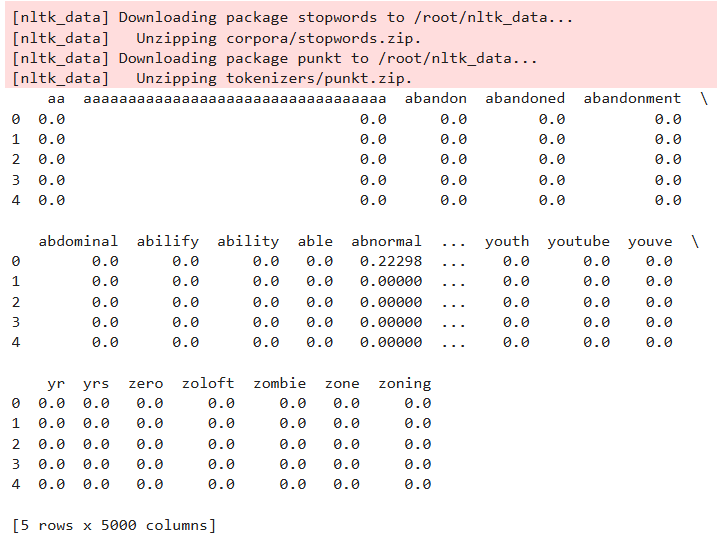
\includegraphics[width=0.8\textwidth]{Images/Output Data Preprocessing.png}  
    \caption{Data Preprocessing}
    \label{Data Preprocessing}  % Label for referencing the figure
\end{figure}

% Bag Of Words Model
\subsubsection{Implementation of Bag Of Words}

\noindent
The following code snippet implements the Bag of Words (BoW) model for the preprocessed dataset related to mental health. This process converts text data into a numerical format that can be used for machine learning tasks.

\begin{verbatim}
import pandas as pd
from sklearn.feature_extraction.text import CountVectorizer
# Load the preprocessed dataset
dataset = pd.read_csv('preprocessed_mental_health_text.csv')
# Check if 'cleaned_text' column exists
if 'cleaned_text' not in dataset.columns:
    raise ValueError("The dataset must have a 'cleaned_text' column. 
    Ensure text preprocessing has been done.")
# Remove rows with missing values in 'cleaned_text' column
dataset.dropna(subset=['cleaned_text'], inplace=True)
# Initialize the CountVectorizer
vectorizer = CountVectorizer()
# Fit and transform the cleaned text data
X = vectorizer.fit_transform(dataset['cleaned_text'])
# Convert the result to a DataFrame for better visualization (optional)
X_df = pd.DataFrame(X.toarray(), columns=vectorizer.
get_feature_names_out())
# Print the shape of the resulting matrix
print(f'Shape of Bag of Words matrix: {X_df.shape}')
# Print the first few rows of the Bag of Words DataFrame (optional)
print(X_df.head())
\end{verbatim}

\noindent
The code begins by importing the necessary libraries: \texttt{pandas} for data manipulation and \texttt{CountVectorizer} from \texttt{sklearn} for creating the Bag of Words model. It then loads a preprocessed dataset from a CSV file named \texttt{preprocessed\_mental\_health\_text.csv}. A check is performed to ensure that the dataset contains a column labeled \texttt{cleaned\_text}. If this column is absent, a \texttt{ValueError} is raised, prompting the user to ensure text preprocessing is completed. Following this, any rows with missing values in the \texttt{cleaned\_text} column are removed to maintain data integrity. Next, an instance of \texttt{CountVectorizer} is initialized, which will convert the cleaned text into a matrix of token counts. The \texttt{fit\_transform()} method is called on the cleaned text data, generating a sparse matrix \(X\) that represents the Bag of Words model. This matrix is then converted into a DataFrame \texttt{X\_df} for easier visualization, with columns corresponding to the unique words identified in the text. Finally, the shape of the resulting Bag of Words matrix is printed to the console, along with the first few rows of the DataFrame to provide a preview of the transformed data.

\begin{figure}[h!]  
    \centering
    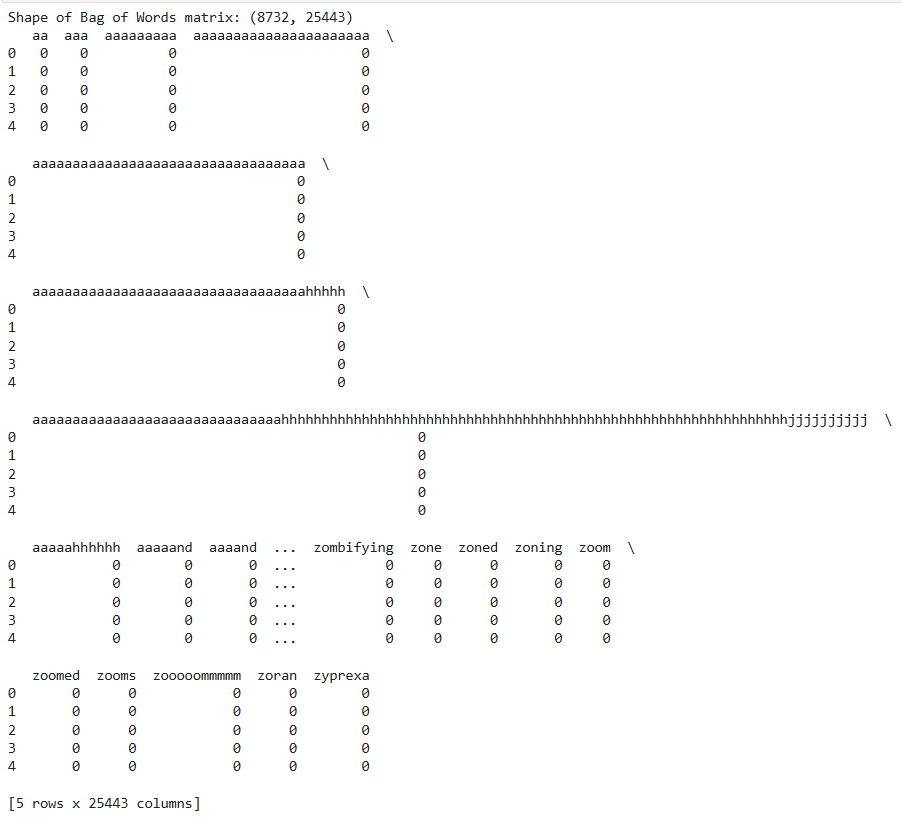
\includegraphics[width=0.8\textwidth]{Images/Output BOW.png}  
    \caption{Implementation of Bag Of Words}
    \label{BOW}  % Label for referencing the figure
\end{figure}

% Splitting DataSet
\subsubsection{Splitting Preprocessed Dataset}
\noindent
The following code snippet demonstrates how to split the preprocessed dataset into training and test sets, which is a crucial step in preparing data for machine learning models.

\begin{verbatim}
import pandas as pd
from sklearn.model_selection import train_test_split

# Load the preprocessed dataset
dataset = pd.read_csv('preprocessed_mental_health_text.csv')

# Check if 'cleaned_text' and 'mental_health_issue' columns exist
if 'cleaned_text' not in dataset.columns or 'mental_health_issue' 
not in dataset.columns:
    raise ValueError("The dataset must have 'cleaned_text' and 
    'mental_health_issue' columns.")

# Remove rows with missing values in 'cleaned_text' column
dataset.dropna(subset=['cleaned_text'], inplace=True) 
#This line has been added

# Initialize the CountVectorizer and fit/transform the cleaned text
from sklearn.feature_extraction.text import CountVectorizer

vectorizer = CountVectorizer()
X = vectorizer.fit_transform(dataset['cleaned_text'])

# Prepare the target variable
y = dataset['mental_health_issue']

# Split the dataset into Training and Test Sets
X_train, X_test, y_train, y_test = train_test_split(X, y, 
test_size=0.2, random_state=42)

# Print the shapes of the resulting datasets
print(f'Shape of X_train: {X_train.shape}')
print(f'Shape of X_test: {X_test.shape}')
print(f'Shape of y_train: {y_train.shape}')
print(f'Shape of y_test: {y_test.shape}')
\end{verbatim}

\noindent
The code begins by importing the necessary libraries, specifically \texttt{pandas} for data manipulation and \texttt{train\_test\_split} from \texttt{sklearn.model\_selection} for splitting the dataset. It then loads 
the preprocessed dataset from a CSV file named \newline
\texttt{preprocessed\_mental\_health\_text.csv}. A validation check is performed to ensure that both the \texttt{cleaned\_text} and 
\texttt{mental\_health\_issue} columns exist in the dataset; if not, a \texttt{ValueError} is raised to alert the user. Next, rows with missing values in the \texttt{cleaned\_text} column are removed to maintain data integrity. After this, the \texttt{CountVectorizer} is initialized to transform the cleaned text into a numerical format suitable for machine learning. The transformed text data is stored in the variable \(X\), while the target variable representing mental health issues is stored in \(y\). The dataset is then split into training and test sets, with 80\% of the data used for training and 20\% for testing, controlled by the \texttt{random\_state} parameter to ensure reproducibility. Finally, the shapes of the resulting training and test datasets are printed to the console, providing insights into the number of samples allocated for training and testing, which is essential for understanding the data distribution.

\begin{figure}[h!]  
    \centering
    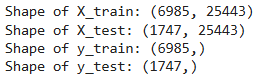
\includegraphics[width=0.6\textwidth]{Images/Output Splitting Dataset.png}  
    \caption{Splitting Dataset}
    \label{Splitting Dataset}  % Label for referencing the figure
\end{figure}


\subsubsection{Logistic Regression}
\noindent
The following code snippet demonstrates the training and evaluation of a Logistic Regression model using a preprocessed dataset related to mental health.

\begin{figure}[h!]  
    \centering
    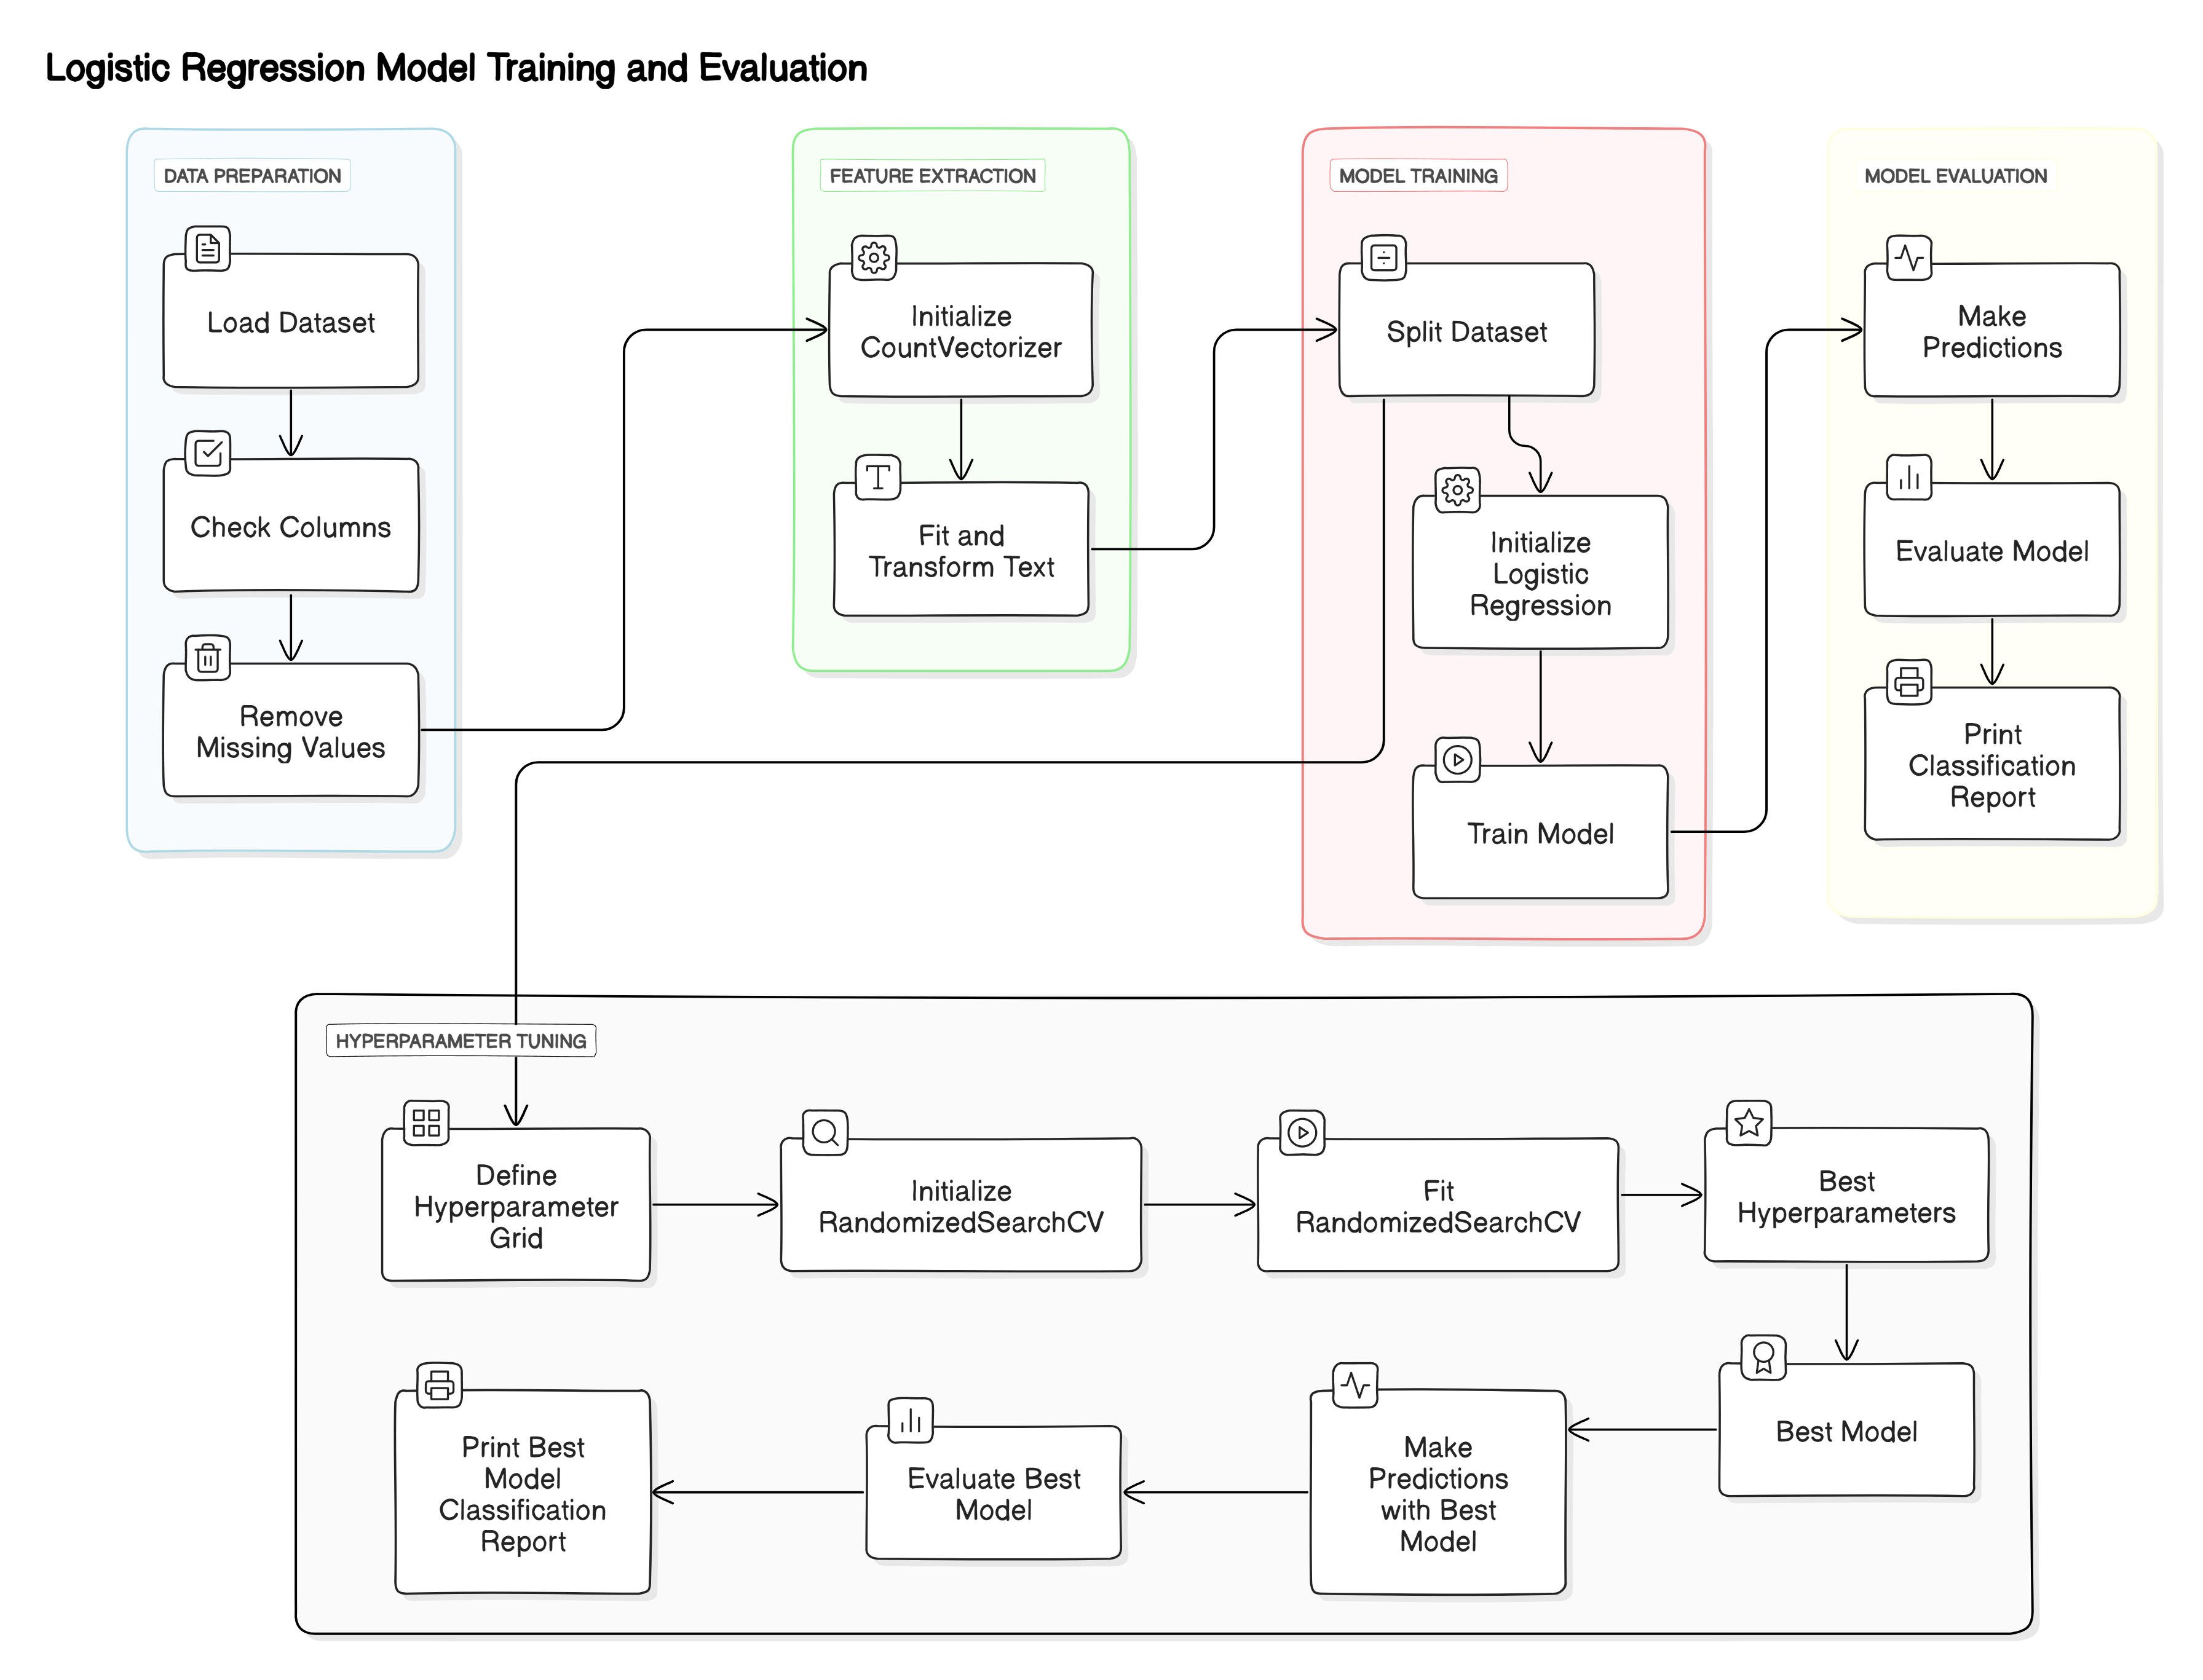
\includegraphics[width=1.0\textwidth]{Images/Logistic Regression.png}  
    \caption{Logistic Regression}
    \label{Logistic Regression}  % Label for referencing the figure
\end{figure}

\begin{verbatim}
import pandas as pd
from sklearn.model_selection import train_test_split
from sklearn.feature_extraction.text import CountVectorizer
from sklearn.linear_model import LogisticRegression
from sklearn.metrics import accuracy_score, classification_report
dataset = pd.read_csv('preprocessed_mental_health_text.csv')
if 'cleaned_text' not in dataset.columns or 'mental_health_issue' 
not in dataset.columns:
    raise ValueError("The dataset must have 'cleaned_text' and 
    'mental_health_issue' columns.")
dataset.dropna(subset=['cleaned_text'], inplace=True)
vectorizer = CountVectorizer()
X = vectorizer.fit_transform(dataset['cleaned_text'])
y = dataset['mental_health_issue']
X_train, X_test, y_train, y_test = train_test_split(X, y, 
test_size=0.2, random_state=42)
model = LogisticRegression(max_iter=2000)
model.fit(X_train, y_train)
y_pred = model.predict(X_test)
accuracy = accuracy_score(y_test, y_pred)
print(f'Accuracy: {accuracy * 100:.2f}%')
print("Classification Report:\n", classification_report(y_test, 
y_pred))
\end{verbatim}

\noindent
The code begins by importing necessary libraries, including \texttt{pandas} for data manipulation and various functions from \texttt{sklearn} for model training and evaluation. It then loads the preprocessed dataset from a CSV file named \texttt{preprocessed\_mental\_health\_text.csv}. A validation check ensures that the dataset contains the required columns, raising an error if either \texttt{cleaned\_text} or \texttt{mental\_health\_issue} is missing. Rows with missing values in the \texttt{cleaned\_text} column are removed to maintain data quality. The \texttt{CountVectorizer} is initialized and used to convert the cleaned text data into a matrix of token counts, stored in \(X\). The target variable, representing mental health issues, is assigned to \(y\). The dataset is then split into training and testing sets, with 80\% used for training and 20\% for testing. A Logistic Regression model is initialized and trained on the training data. Predictions are made on the test set, and the model's accuracy is calculated and printed. Finally, a classification report is generated, providing detailed metrics on the model’s performance across different categories.

\begin{figure}[h!]  
    \centering
    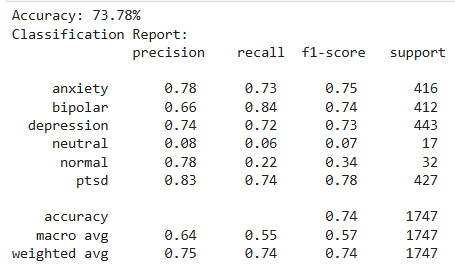
\includegraphics[width=0.8\textwidth]{Images/Output Logistic Regression.png}  
    \caption{Logistic Regression Result}
    \label{Logistic Regression Result}  % Label for referencing the figure
\end{figure}

\subsubsection{Hyperparameter Tuning on Logistic Regression using Random Search}

The following code snippet demonstrates how to perform hyperparameter tuning on a Logistic Regression model using Random Search.

\begin{verbatim}
import pandas as pd
from sklearn.model_selection import train_test_split, 
RandomizedSearchCV
from sklearn.feature_extraction.text import CountVectorizer
from sklearn.linear_model import LogisticRegression
from sklearn.metrics import accuracy_score, classification_report
dataset = pd.read_csv('preprocessed_mental_health_text.csv')
if 'cleaned_text' not in dataset.columns or 'mental_health_issue' 
not in dataset.columns:
    raise ValueError("The dataset must have 'cleaned_text' and 
    'mental_health_issue' columns.")
dataset.dropna(subset=['cleaned_text'], inplace=True)
vectorizer = CountVectorizer()
X = vectorizer.fit_transform(dataset['cleaned_text'])
y = dataset['mental_health_issue']
X_train, X_test, y_train, y_test = train_test_split(X, y, 
test_size=0.2, random_state=42)
model = LogisticRegression(max_iter=200)
param_distributions = {
    'C': [0.001, 0.01, 0.1, 1, 10, 100],
    'penalty': ['l1', 'l2', 'elasticnet', 'none'],
    'solver': ['liblinear', 'saga']
}
random_search = RandomizedSearchCV(estimator=model, 
param_distributions=param_distributions,
n_iter=10, scoring='accuracy', cv=5, n_jobs=-1, random_state=42)
random_search.fit(X_train, y_train)
print("Best Hyperparameters:", random_search.best_params_)
best_model = random_search.best_estimator_
y_pred = best_model.predict(X_test)
accuracy = accuracy_score(y_test, y_pred)
print(f'Accuracy: {accuracy * 100:.2f}%')
print("Classification Report:\n", 
classification_report(y_test, y_pred))
\end{verbatim}

\noindent
The code begins by importing the necessary libraries, including \texttt{pandas} for data manipulation and various functions from \texttt{sklearn} for model training and evaluation. It loads the preprocessed dataset from a CSV file named \newline \texttt{preprocessed\_mental\_health\_text.csv} and checks for the required columns \texttt{cleaned\_text} and \texttt{mental\_health\_issue}. If these columns are not present, a \texttt{ValueError} is raised. The code then removes any rows with missing values in the \texttt{cleaned\_text} column. The \texttt{CountVectorizer} is initialized to convert the cleaned text into a numerical format, which is stored in \(X\), while the target variable representing mental health issues is stored in \(y\). The dataset is split into training and testing sets with 80\% for training and 20\% for testing. A Logistic Regression model is created with a maximum of 200 iterations. The hyperparameter grid for tuning is defined, specifying values for the inverse of regularization strength (\texttt{C}), types of regularization (\texttt{penalty}), and solvers. A \texttt{RandomizedSearchCV} object is initialized to perform the random search over the hyperparameter grid, and the model is fitted using the training data. The best hyperparameters are printed, and the best model is used to make predictions on the test set. Finally, the model's accuracy is calculated and displayed, along with a classification report that provides detailed metrics on the model's performance across different categories.

\begin{figure}[h!]  
    \centering
    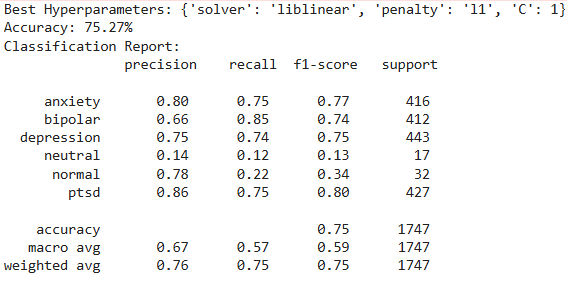
\includegraphics[width=0.6\textwidth]{Images/Output HPT LR.png}  
    \caption{Result of Hyperparameter Tuning on Logistic Regression}
    \label{Project Modules}  % Label for referencing the figure
\end{figure}

\begin{figure}[h!]  
    \centering
    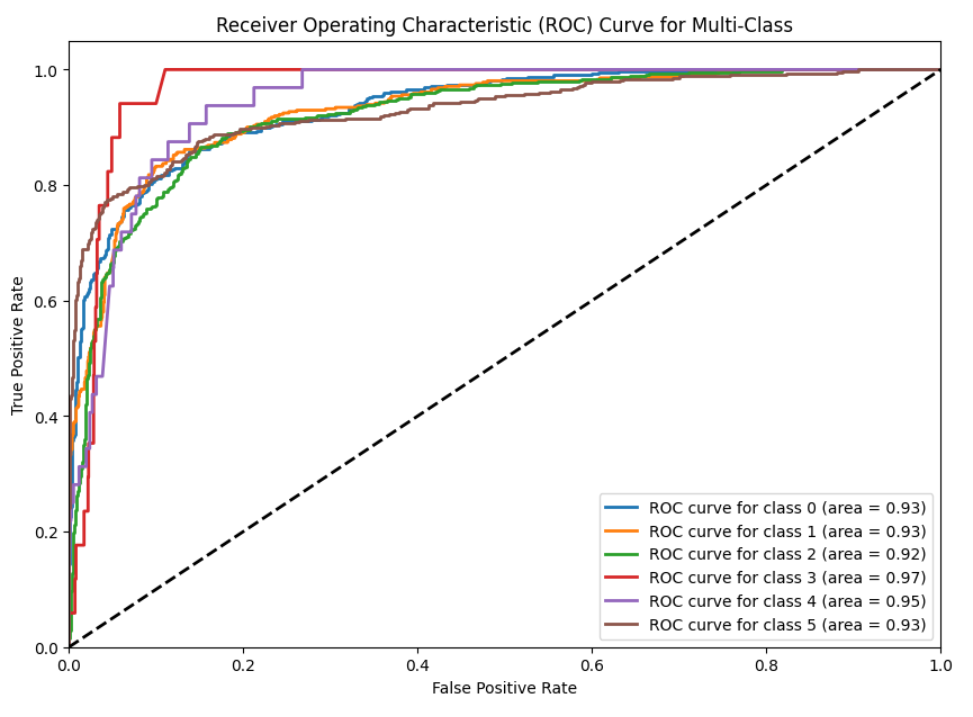
\includegraphics[width=0.6\textwidth]{Images/ROC LR.png}  
    \caption{ROC Curve on Logistic Regression}
    \label{ROC LR}  % Label for referencing the figure
\end{figure}


\subsubsection{K Nearest Neighbours}
\noindent
The following code snippet demonstrates the implementation of the k-Nearest Neighbors (k-NN) algorithm for classifying mental health issues based on preprocessed text data.

\begin{figure}[h!]  
    \centering
    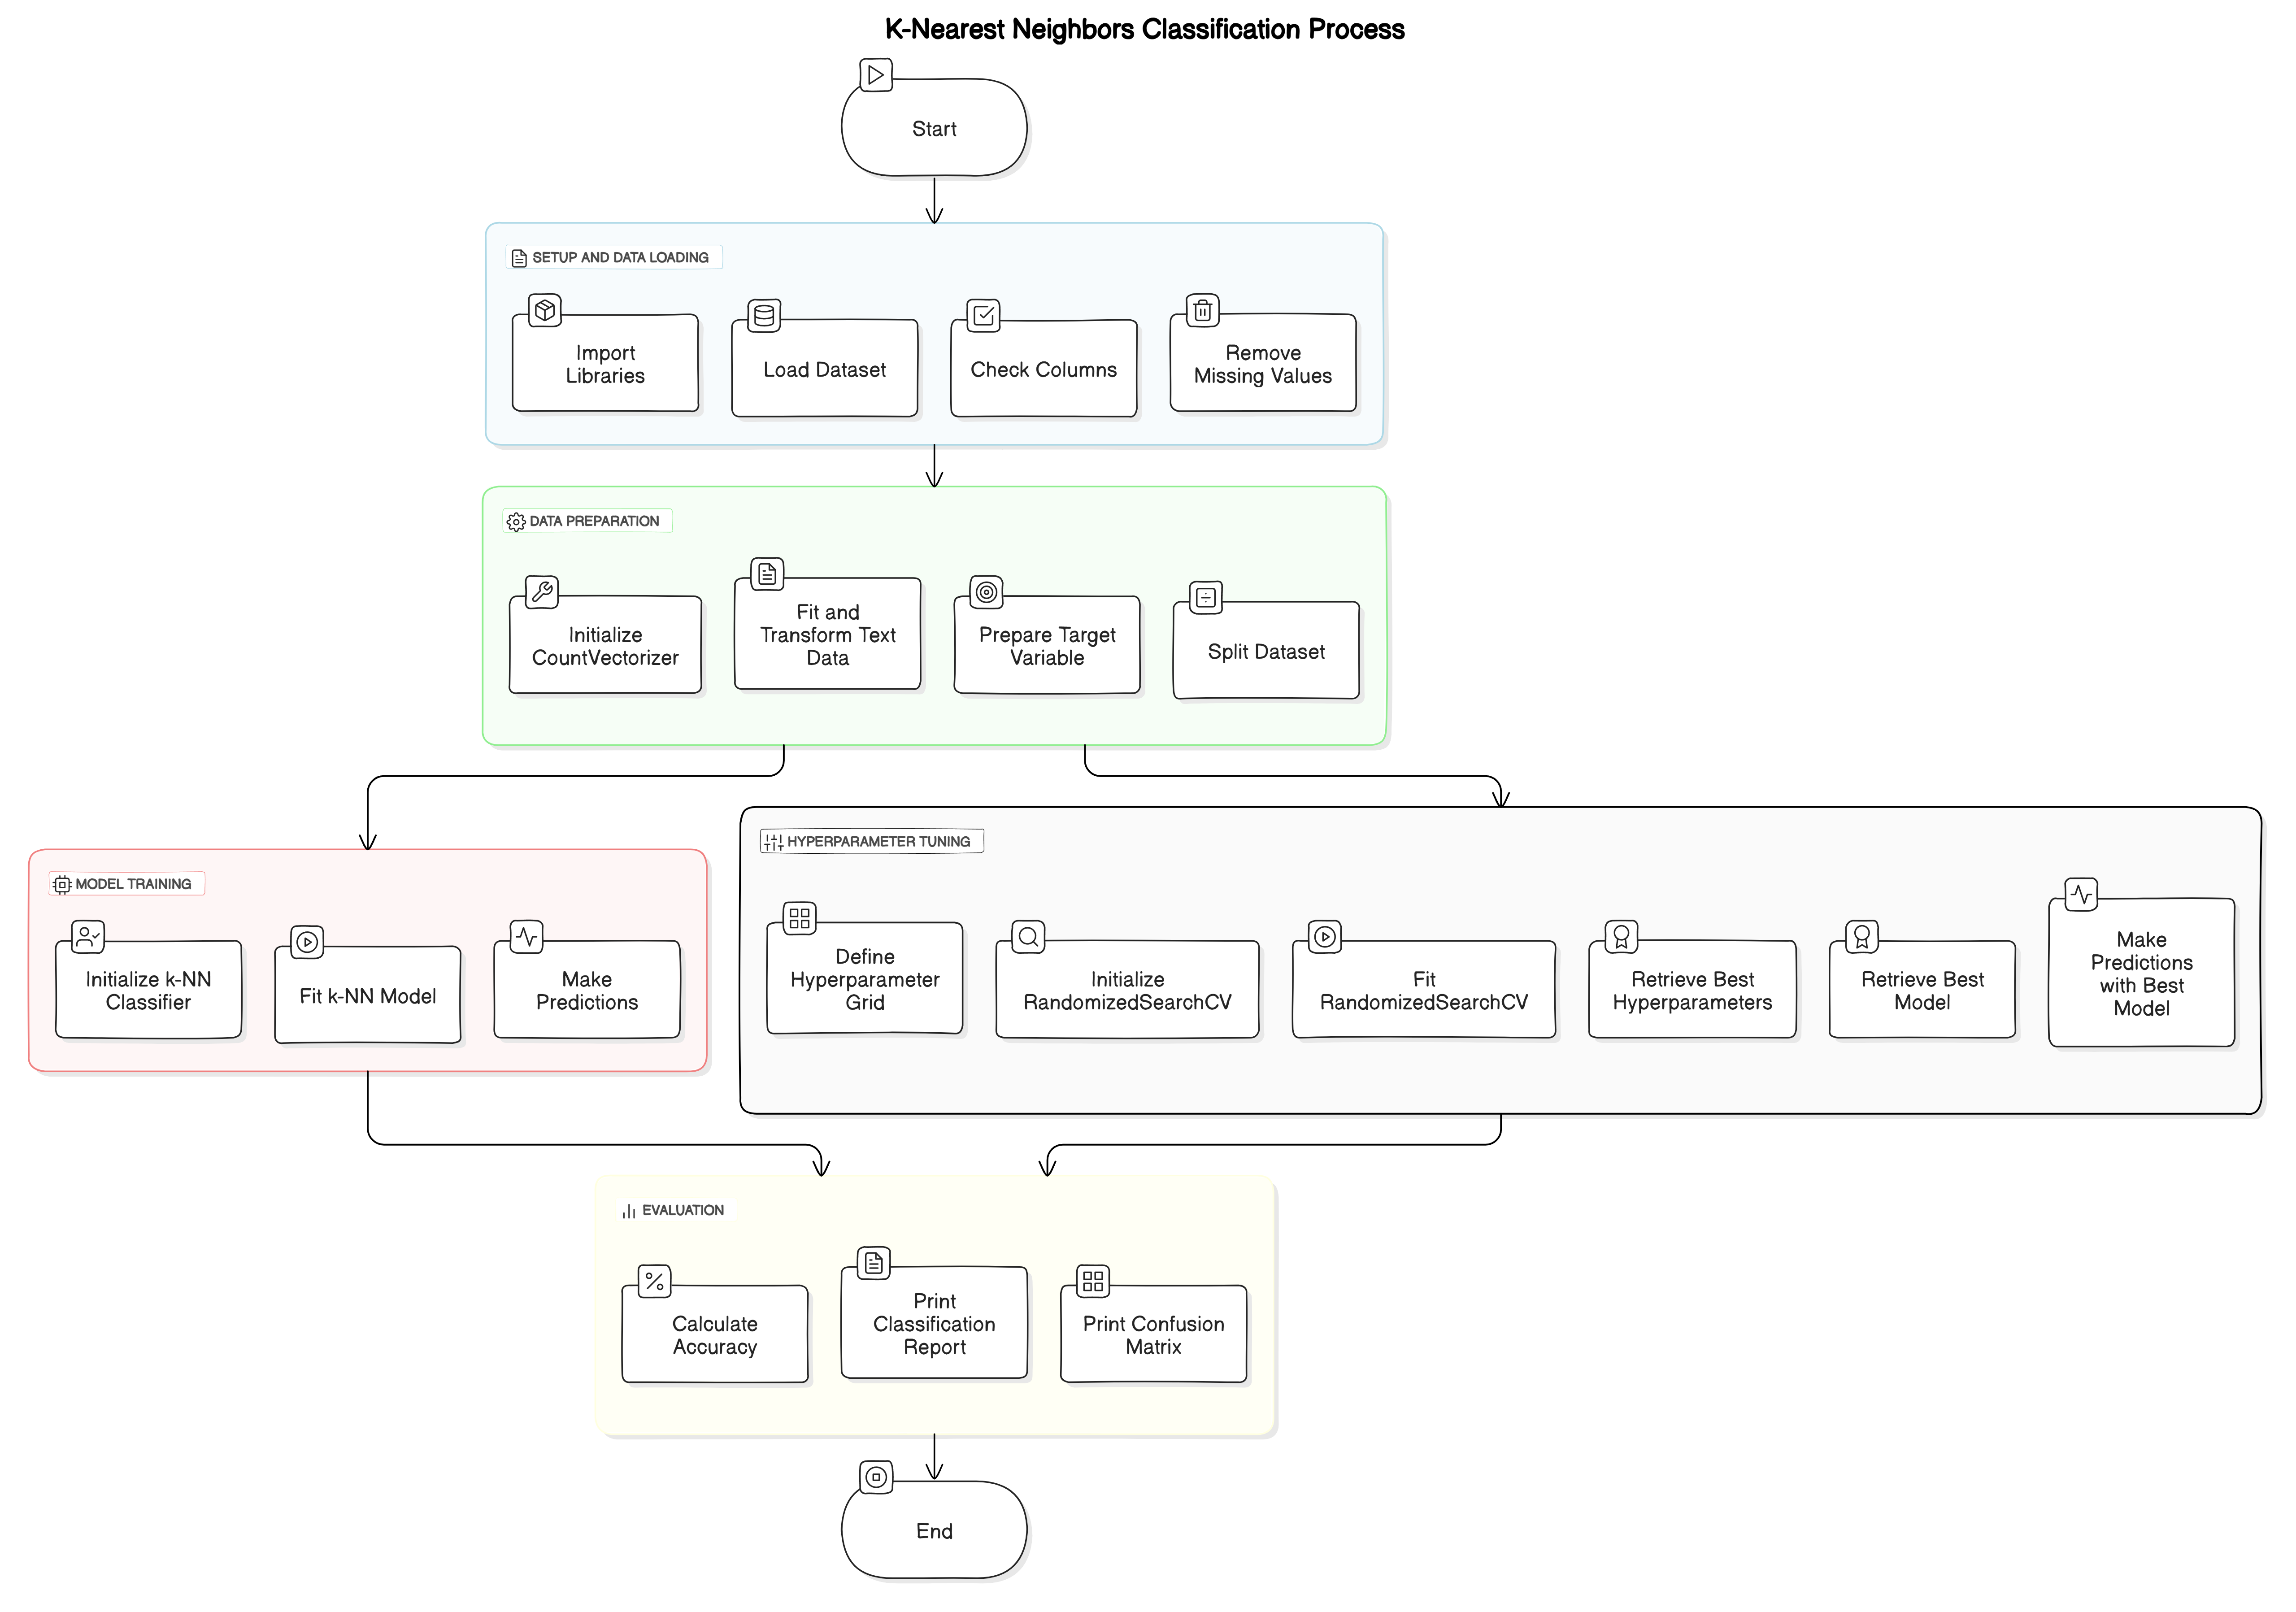
\includegraphics[width=1.0\textwidth]{Images/KNN.png}  
    \caption{K Nearest Neighbours Workflow}
    \label{KNN}  % Label for referencing the figure
\end{figure}


\begin{verbatim}
import pandas as pd
from sklearn.model_selection import train_test_split
from sklearn.feature_extraction.text import CountVectorizer
from sklearn.neighbors import KNeighborsClassifier
from sklearn.metrics import accuracy_score, classification_report, 
confusion_matrix
dataset = pd.read_csv('preprocessed_mental_health_text.csv')
if 'cleaned_text' not in dataset.columns or 'mental_health_issue' 
not in dataset.columns:
    raise ValueError("The dataset must have 'cleaned_text' and 
    'mental_health_issue' columns.")
dataset.dropna(subset=['cleaned_text'], inplace=True)
vectorizer = CountVectorizer()
X = vectorizer.fit_transform(dataset['cleaned_text'])
y = dataset['mental_health_issue']
X_train, X_test, y_train, y_test = train_test_split(X, y, 
test_size=0.2, random_state=42)
knn = KNeighborsClassifier(n_neighbors=5)
knn.fit(X_train, y_train)
y_pred = knn.predict(X_test)
accuracy = accuracy_score(y_test, y_pred)
print(f'Accuracy: {accuracy * 100:.2f}%')
print("Classification Report:\n", 
classification_report(y_test, y_pred))
print("Confusion Matrix:\n", confusion_matrix(y_test,y_pred))
\end{verbatim}

\noindent
The code begins by importing the necessary libraries, including \texttt{pandas} for data manipulation, \texttt{train\_test\_split} for splitting the dataset, \texttt{CountVectorizer} for transforming text data, and \texttt{KNeighborsClassifier} along with various metrics from \texttt{sklearn} for model evaluation. It loads the preprocessed dataset from a CSV file named \newline
\texttt{preprocessed\_mental\_health\_text.csv} and checks that both the \texttt{cleaned\_text} and \texttt{mental\_health\_issue} columns are present; if not, a \texttt{ValueError} is raised. Rows with missing values in the \texttt{cleaned\_text} column are removed to maintain data integrity. The \texttt{CountVectorizer} is initialized to convert the cleaned text into a numerical format, stored in \(X\), while the target variable representing mental health issues is assigned to \(y\). The dataset is split into training and testing sets, with 80\% used for training and 20\% for testing. A k-NN classifier is initialized with 5 neighbors, and the model is fitted on the training data. Predictions are made on the test set, and the model's accuracy is calculated and displayed. Finally, a classification report and confusion matrix are printed, providing detailed metrics on the model's performance and insight into its classification results.

\begin{figure}[h!]  
    \centering
    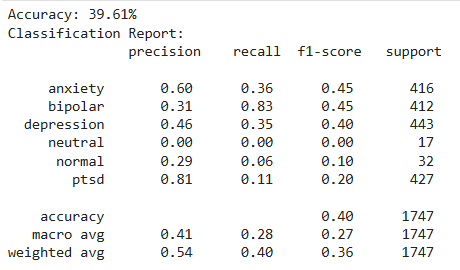
\includegraphics[width=0.6\textwidth]{Images/Output KNN.png}  
    \caption{K Nearest Neighbours Result}
    \label{KNN}  % Label for referencing the figure
\end{figure}

\subsubsection{Hyperparameter Tuning on KNN Using Random Search}
\noindent
The following code snippet demonstrates how to perform hyperparameter tuning on a k-Nearest Neighbors (k-NN) classifier using Random Search to optimize its performance.

\begin{verbatim}
import pandas as pd
from sklearn.model_selection import train_test_split, 
RandomizedSearchCV
from sklearn.feature_extraction.text import CountVectorizer
from sklearn.neighbors import KNeighborsClassifier
from sklearn.metrics import accuracy_score, classification_report, 
confusion_matrix
dataset = pd.read_csv('preprocessed_mental_health_text.csv')
if 'cleaned_text' 
not in dataset.columns or 'mental_health_issue' not in dataset.columns:
    raise ValueError("The dataset must have 'cleaned_text' and 
    'mental_health_issue' columns.")
dataset.dropna(subset=['cleaned_text'], inplace=True)
vectorizer = CountVectorizer()
X = vectorizer.fit_transform(dataset['cleaned_text'])
y = dataset['mental_health_issue']
X_train, X_test, y_train, y_test = train_test_split(X, y, 
test_size=0.2, random_state=42)
knn = KNeighborsClassifier()
param_distributions = {
    'n_neighbors': [3, 4, 5, 6, 7, 8, 9, 10, 11, 12, 13, 
    14, 15, 16, 17, 18, 19, 20],
    'metric': ['euclidean', 'manhattan', 'chebyshev', 'minkowski'],
    'weights': ['uniform', 'distance']
}
random_search = RandomizedSearchCV(estimator=knn, 
param_distributions=param_distributions, 
n_iter=200, scoring='accuracy', cv=5, n_jobs=-1, random_state=42)
random_search.fit(X_train, y_train)
print("Best Hyperparameters:", random_search.best_params_)
best_knn = random_search.best_estimator_
y_pred = best_knn.predict(X_test)
accuracy = accuracy_score(y_test, y_pred)
print(f'Accuracy: {accuracy * 100:.2f}%')
print("Classification Report:\n", 
classification_report(y_test, y_pred))
print("Confusion Matrix:\n", confusion_matrix(y_test, y_pred))
\end{verbatim}

\noindent
The code starts by importing the required libraries, including \texttt{pandas} for data manipulation, and various functions from \texttt{sklearn} for model training, evaluation, and hyperparameter tuning. It loads the preprocessed dataset from a CSV file named \newline \texttt{preprocessed\_mental\_health\_text.csv} and checks for the presence of the necessary columns, raising a \texttt{ValueError} if they are missing. Rows with missing values in the \texttt{cleaned\_text} column are removed to ensure data quality. The \texttt{CountVectorizer} is initialized to convert the cleaned text into a numerical format, stored in \(X\), while the target variable representing mental health issues is assigned to \(y\). The dataset is split into training and testing sets, with 80\% used for training and 20\% for testing. A k-NN classifier is initialized, and a hyperparameter grid is defined, specifying different values for the number of neighbors, distance metrics, and weighting options for the neighbors. The \texttt{RandomizedSearchCV} object is created to perform random search over the hyperparameter grid, and the model is fitted using the training data. After fitting, the best hyperparameters are printed, along with the best k-NN model derived from the search. Predictions are made on the test set, and the accuracy of the model is calculated and displayed. Finally, a classification report and confusion matrix are printed to evaluate the model's performance and provide insights into its classification results.

\begin{figure}[h!]  
    \centering
    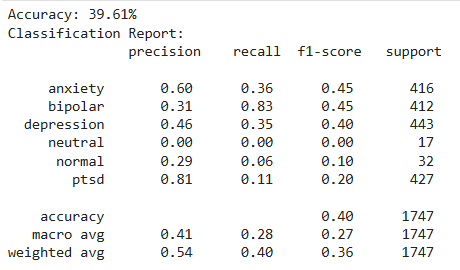
\includegraphics[width=0.8\textwidth]{Images/Output KNN.png}  
    \caption{Result of Hyperparameter Tuning on KNN}
    \label{HPT KNN}  % Label for referencing the figure
\end{figure}

\begin{figure}[h!]  
    \centering
    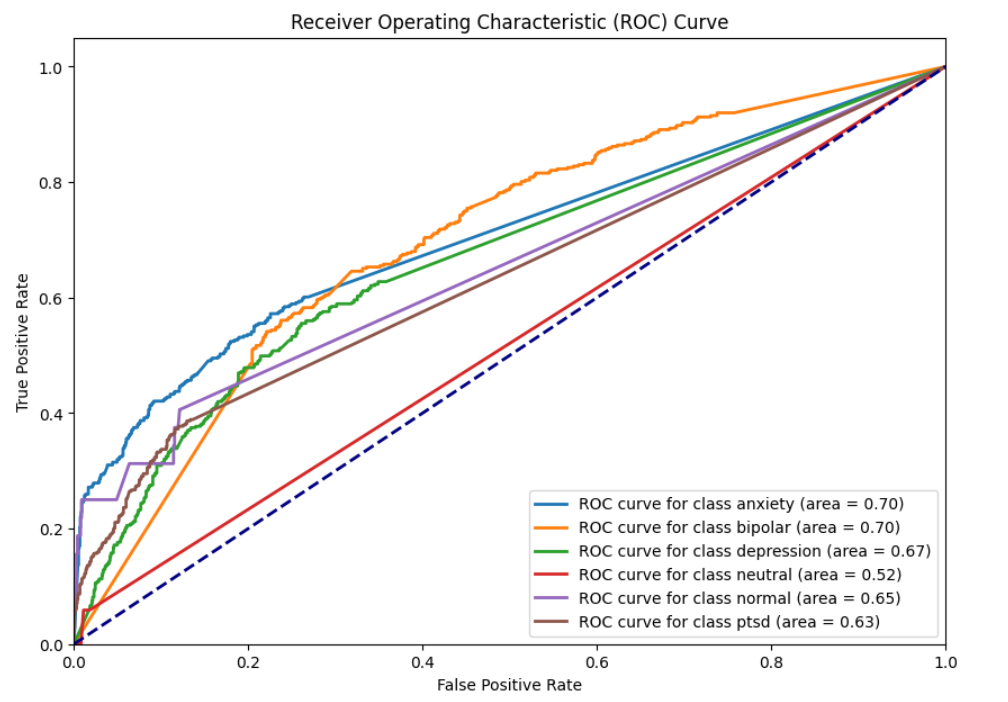
\includegraphics[width=0.8\textwidth]{Images/ROC KNN.png}  
    \caption{ROC curve on KNN}
    \label{ROC KNN}  % Label for referencing the figure
\end{figure}


\subsubsection{Support Vector Machine}
\noindent
The following code snippet demonstrates the implementation of a Support Vector Machine (SVM) classifier for classifying mental health issues based on preprocessed text data.

\begin{figure}[h!]  
    \centering
    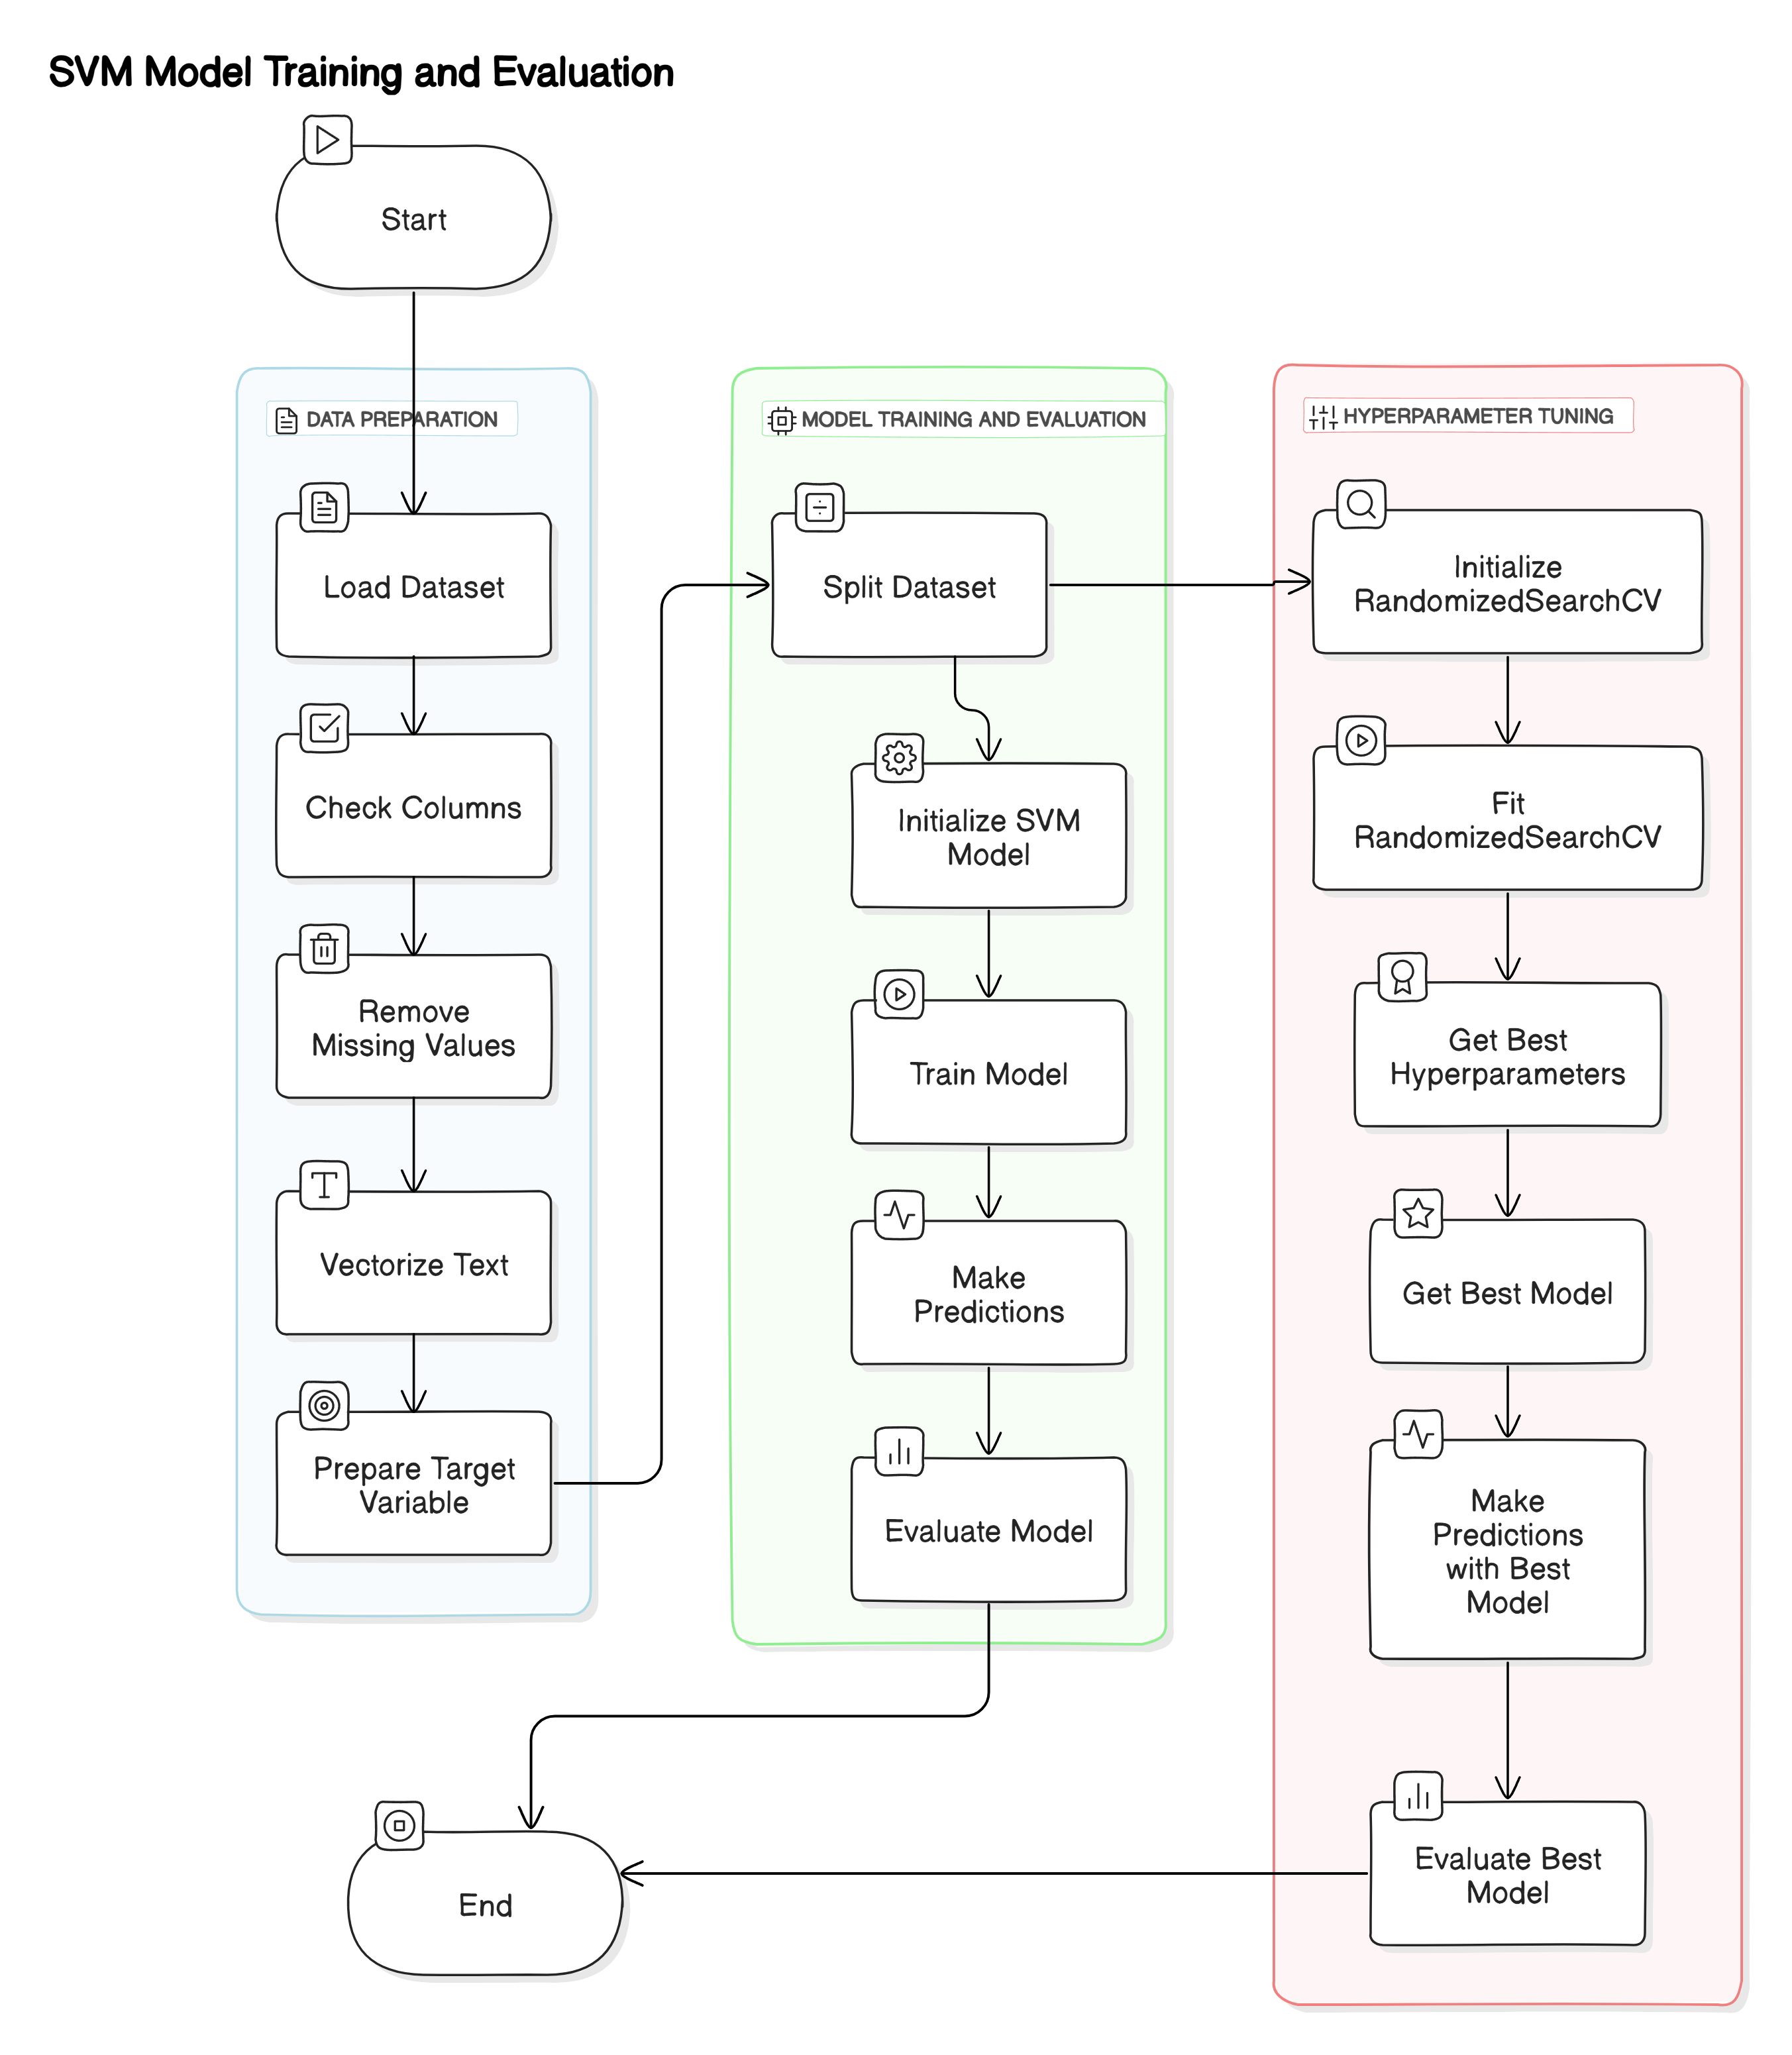
\includegraphics[width=0.6\textwidth]{Images/SVM.png}  
    \caption{Support Vector Machine Workflow}
    \label{SVM}  % Label for referencing the figure
\end{figure}

\begin{verbatim}
import pandas as pd
from sklearn.model_selection import train_test_split
from sklearn.feature_extraction.text import CountVectorizer
from sklearn.svm import SVC
from sklearn.metrics import accuracy_score, classification_report, 
confusion_matrix
dataset = pd.read_csv('preprocessed_mental_health_text.csv')
if 'cleaned_text' not in dataset.columns or 'mental_health_issue' 
not in dataset.columns:
    raise ValueError("The dataset must have 'cleaned_text' and 
    'mental_health_issue' columns.")
dataset.dropna(subset=['cleaned_text'], inplace=True)
vectorizer = CountVectorizer()
X = vectorizer.fit_transform(dataset['cleaned_text'])
y = dataset['mental_health_issue']
X_train, X_test, y_train, y_test = train_test_split(X, y, 
test_size=0.2, random_state=42)
svm_model = SVC(kernel='linear', C=1, random_state=42)
svm_model.fit(X_train, y_train)
y_pred = svm_model.predict(X_test)
accuracy = accuracy_score(y_test, y_pred)
print(f'Accuracy: {accuracy * 100:.2f}%')
print("Classification Report:\n", 
classification_report(y_test, y_pred))
print("Confusion Matrix:\n", confusion_matrix(y_test, y_pred))
\end{verbatim}

\noindent
The code begins by importing the necessary libraries, including \texttt{pandas} for data manipulation and various functions from \texttt{sklearn} for model training and evaluation. It loads the preprocessed dataset from a CSV file named \newline \texttt{preprocessed\_mental\_health\_text.csv} and verifies that both the \texttt{cleaned\_text} and \texttt{mental\_health\_issue} columns exist, raising a \texttt{ValueError} if they are missing. Rows with missing values in the \texttt{cleaned\_text} column are removed to maintain data quality. The \texttt{CountVectorizer} is initialized to convert the cleaned text into a numerical format, stored in \(X\), while the target variable representing mental health issues is assigned to \(y\). The dataset is then split into training and testing sets, with 80\% used for training and 20\% for testing. An SVM model is initialized with a linear kernel and a regularization parameter \(C\) set to 1, which can be adjusted based on the specific needs of the analysis. The model is trained using the training data, and predictions are made on the test set. The accuracy of the model is calculated and displayed, along with a classification report and confusion matrix, which provide insights into the model's performance across different categories and the distribution of classification results.

\begin{figure}[h!]  
    \centering
    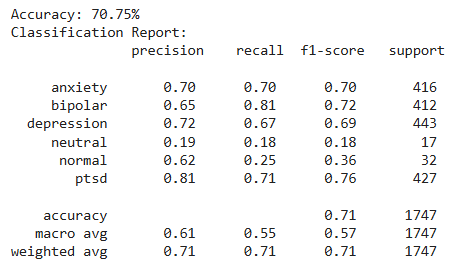
\includegraphics[width=0.6\textwidth]{Images/Output SVM.png}  
    \caption{Support Vector Machine (Linear Kernel) Result}
    \label{SVM}  % Label for referencing the figure
\end{figure}

\subsubsection{Hyperparameter Tuning on SVM using Random Search}
\noindent
The following code snippet demonstrates how to perform hyperparameter tuning on a Support Vector Machine (SVM) classifier using Random Search to optimize its performance.

\begin{verbatim}
import pandas as pd
from sklearn.model_selection import train_test_split, 
RandomizedSearchCV
from sklearn.feature_extraction.text import CountVectorizer
from sklearn.svm import SVC
from sklearn.metrics import accuracy_score, classification_report
dataset = pd.read_csv('preprocessed_mental_health_text.csv')
if 'cleaned_text' not in dataset.columns or 'mental_health_issue'
not in dataset.columns:
    raise ValueError("The dataset must have 'cleaned_text' and 
    'mental_health_issue' columns.")
dataset.dropna(subset=['cleaned_text'], inplace=True)
vectorizer = CountVectorizer()
X = vectorizer.fit_transform(dataset['cleaned_text'])
y = dataset['mental_health_issue']
X_train, X_test, y_train, y_test = train_test_split(X, y, 
test_size=0.2, random_state=42)
model = SVC()
param_distributions = {
    'C': [0.1, 1, 10, 100],
    'kernel': ['linear', 'rbf', 'poly'],
    'gamma': ['scale', 'auto', 0.1, 1],
}
random_search = RandomizedSearchCV(estimator=model, 
param_distributions=param_distributions, 
n_iter=200, scoring='accuracy', 
cv=5, n_jobs=-1, random_state=42)
random_search.fit(X_train, y_train)
print("Best Hyperparameters:", random_search.best_params_)
best_model = random_search.best_estimator_
y_pred = best_model.predict(X_test)
accuracy = accuracy_score(y_test, y_pred)
print(f'Accuracy: {accuracy * 100:.2f}%')
print("Classification Report:\n", 
classification_report(y_test, y_pred))
\end{verbatim}

\noindent
The code begins by importing the required libraries, including \texttt{pandas} for data manipulation and various functions from \texttt{sklearn} for model training and evaluation. It loads the preprocessed dataset from a CSV file named \newline \texttt{preprocessed\_mental\_health\_text.csv} and checks for the necessary columns, raising a \texttt{ValueError} if either the \texttt{cleaned\_text} or \texttt{mental\_health\_issue} columns are missing. Rows with missing values in the \texttt{cleaned\_text} column are then removed to ensure data quality. The \texttt{CountVectorizer} is initialized to convert the cleaned text into a numerical format, stored in \(X\), while the target variable representing mental health issues is assigned to \(y\). The dataset is split into training and testing sets, with 80\% used for training and 20\% for testing. An SVM model is initialized, and a hyperparameter grid is defined that specifies different values for the regularization parameter \(C\), various kernel types, and kernel coefficients. The \texttt{RandomizedSearchCV} object is created to perform random search over the hyperparameter grid, and the model is fitted using the training data. After fitting, the best hyperparameters are printed along with the best SVM model derived from the search. Predictions are made on the test set, and the accuracy of the model is calculated and displayed, along with a classification report that provides detailed metrics on the model's performance.

\begin{figure}[h!]  
    \centering
    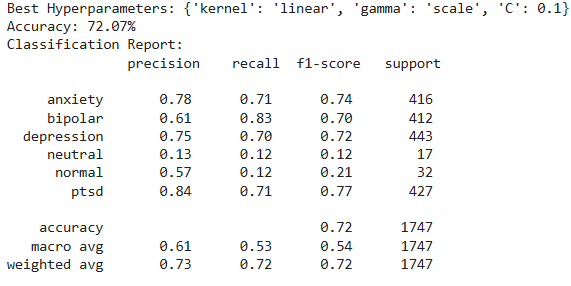
\includegraphics[width=0.8\textwidth]{Images/Output HPT SVM.png}  
    \caption{Result of Hyperparameter Tuning on SVM}
    \label{HPT SVM}  % Label for referencing the figure
\end{figure}

\begin{figure}[h!]  
    \centering
    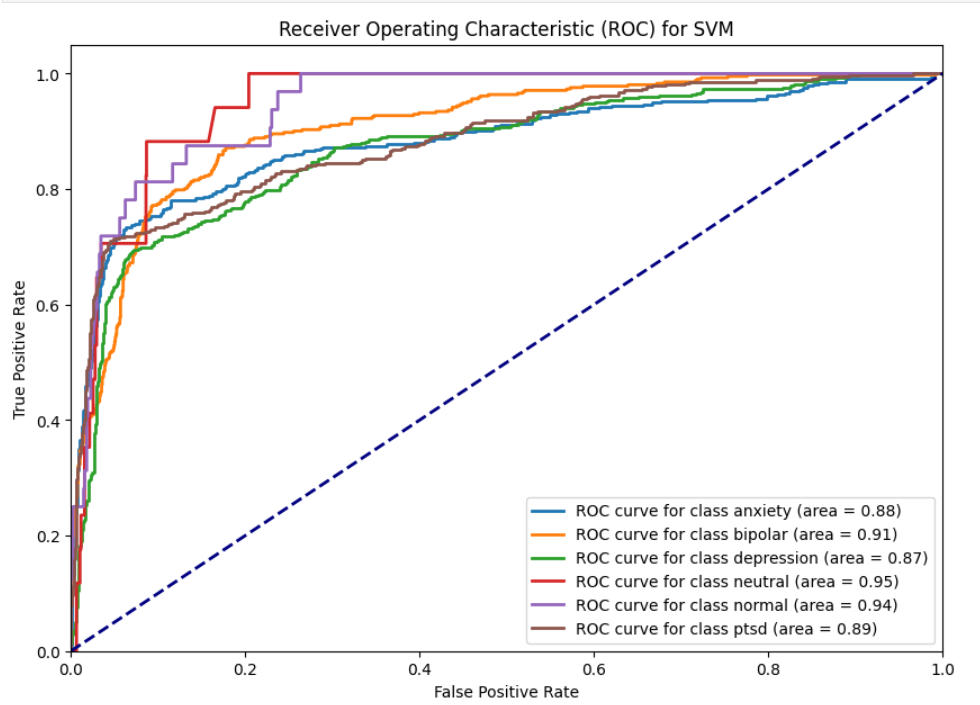
\includegraphics[width=0.8\textwidth]{Images/ROC SVM.png}  
    \caption{ROC Curve on SVM}
    \label{ROC SVM}  % Label for referencing the figure
\end{figure}

\pagebreak

\subsubsection{Naive Bayes Result}
\noindent
The following code snippet demonstrates the implementation of a Naive Bayes classifier for classifying mental health issues based on preprocessed text data.

\begin{figure}[h!]  
    \centering
    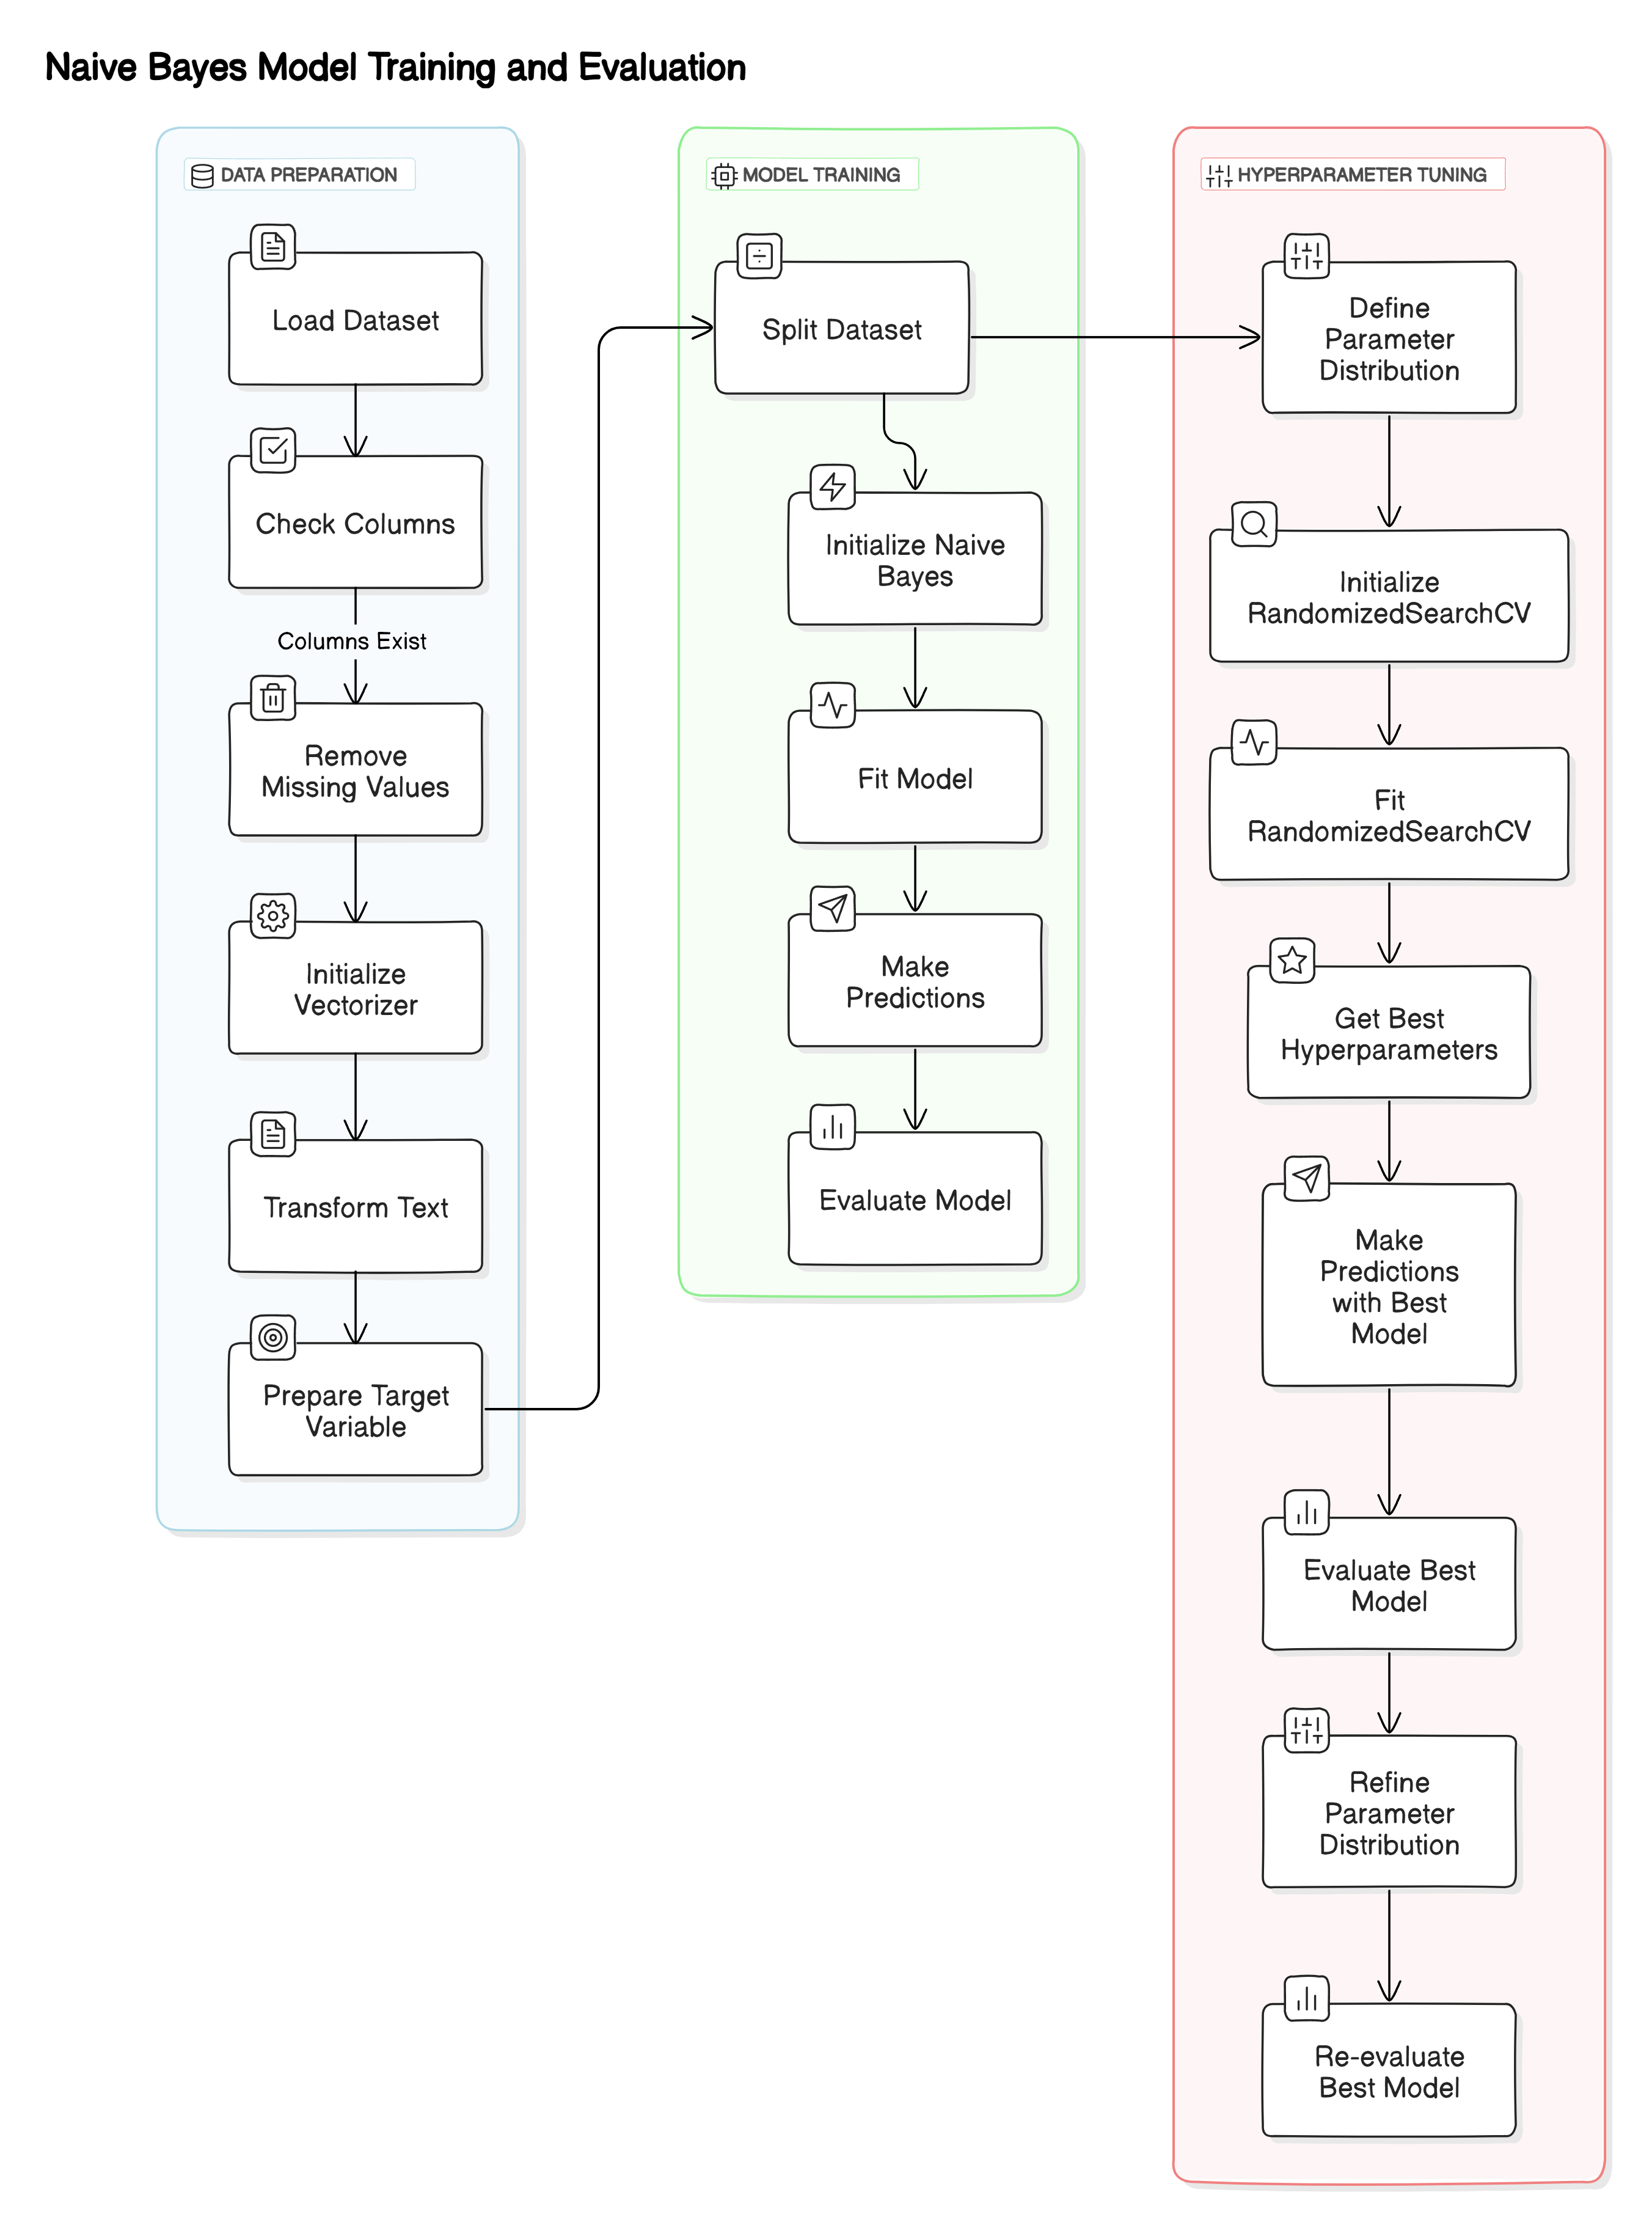
\includegraphics[width=1.0\textwidth]{Images/Naive Bayes.png}  
    \caption{Naive Bayes Workflow}
    \label{Naive Bayes}  % Label for referencing the figure
\end{figure}

\begin{verbatim}
import pandas as pd
from sklearn.model_selection import train_test_split
from sklearn.feature_extraction.text import CountVectorizer
from sklearn.naive_bayes import MultinomialNB
from sklearn.metrics import accuracy_score, classification_report, 
confusion_matrix
dataset = pd.read_csv('preprocessed_mental_health_text.csv')
if 'cleaned_text' not in dataset.columns or 'mental_health_issue' 
not in dataset.columns:
    raise ValueError("The dataset must have 'cleaned_text' and 
    'mental_health_issue' columns.")
dataset.dropna(subset=['cleaned_text'], inplace=True)
vectorizer = CountVectorizer()
X = vectorizer.fit_transform(dataset['cleaned_text'])
y = dataset['mental_health_issue']
X_train, X_test, y_train, y_test = train_test_split(X, y, 
test_size=0.2, random_state=42)
naive_bayes_model = MultinomialNB()
naive_bayes_model.fit(X_train, y_train)
y_pred = naive_bayes_model.predict(X_test)
accuracy = accuracy_score(y_test, y_pred)
print(f'Accuracy: {accuracy * 100:.2f}%')
print("Classification Report:\n", 
classification_report(y_test, y_pred))
print("Confusion Matrix:\n", confusion_matrix(y_test, y_pred))
\end{verbatim}

\noindent
The code begins by importing the necessary libraries, including \texttt{pandas} for data manipulation and various functions from \texttt{sklearn} for model training and evaluation. It loads the preprocessed dataset from a CSV file named \newline
\texttt{preprocessed\_mental\_health\_text.csv} and checks for the required columns, raising a \texttt{ValueError} if either the \texttt{cleaned\_text} or \texttt{mental\_health\_issue} columns are missing. Rows with missing values in the \texttt{cleaned\_text} column are then removed to ensure data quality. The \texttt{CountVectorizer} is initialized to convert the cleaned text into a numerical format, which is stored in \(X\), while the target variable representing mental health issues is assigned to \(y\). The dataset is split into training and testing sets, with 80\% used for training and 20\% for testing. A Naive Bayes classifier, specifically \texttt{MultinomialNB}, is initialized and fitted using the training data. Predictions are made on the test set, and the model's accuracy is calculated and displayed. Finally, a classification report and confusion matrix are printed, providing detailed metrics on the model's performance across different categories and insights into its classification results.

\begin{figure}[h!]  
    \centering
    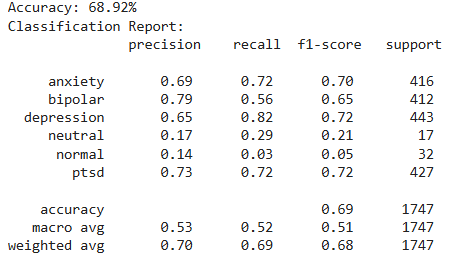
\includegraphics[width=0.8\textwidth]{Images/Output NB.png}  
    \caption{Naive Bayes}
    \label{NB}  % Label for referencing the figure
\end{figure}

\subsubsection{Hyperparameter Tuning on Naive Bayes using Random Search}
\noindent
The following code snippet demonstrates how to perform hyperparameter tuning on a Naive Bayes classifier using Random Search to optimize its performance.

\begin{verbatim}
import pandas as pd
from sklearn.model_selection import train_test_split, 
RandomizedSearchCV
from sklearn.feature_extraction.text import CountVectorizer
from sklearn.naive_bayes import MultinomialNB
from sklearn.metrics import accuracy_score, classification_report, 
confusion_matrix
from scipy.stats import uniform
dataset = pd.read_csv('preprocessed_mental_health_text.csv')
if 'cleaned_text' not in dataset.columns or 'mental_health_issue' 
not in dataset.columns:
    raise ValueError("The dataset must have 'cleaned_text' and 
    'mental_health_issue' columns.")
dataset.dropna(subset=['cleaned_text'], inplace=True)
vectorizer = CountVectorizer()
X = vectorizer.fit_transform(dataset['cleaned_text'])
y = dataset['mental_health_issue']
X_train, X_test, y_train, y_test = train_test_split(X, y, 
test_size=0.2, random_state=42)
naive_bayes_model = MultinomialNB()
param_distributions = {
    'alpha': uniform(0.001, 5.0)
}
random_search = RandomizedSearchCV(estimator=naive_bayes_model, 
param_distributions=param_distributions, n_iter=2000, 
scoring='accuracy', cv=5, n_jobs=-1, random_state=42)
random_search.fit(X_train, y_train)
print("Best Hyperparameters:", random_search.best_params_)
best_model = random_search.best_estimator_
y_pred = best_model.predict(X_test)
accuracy = accuracy_score(y_test, y_pred)
print(f'Accuracy: {accuracy * 100:.2f}%')
print("Classification Report:\n", 
classification_report(y_test, y_pred))
print("Confusion Matrix:\n", confusion_matrix(y_test, y_pred))
\end{verbatim}

\noindent
The code begins by importing the necessary libraries, including \texttt{pandas} for data manipulation, various functions from \texttt{sklearn} for model training and evaluation, and \texttt{uniform} from \texttt{scipy.stats} for sampling. It loads the preprocessed dataset from a CSV file named \texttt{preprocessed\_mental\_health\_text.csv} and checks for the presence of the required columns, raising a \texttt{ValueError} if either the \texttt{cleaned\_text} or \texttt{mental\_health\_issue} columns are missing. Rows with missing values in the \texttt{cleaned\_text} column are removed to maintain data quality. The \texttt{CountVectorizer} is initialized to convert the cleaned text into a numerical format, which is stored in \(X\), while the target variable representing mental health issues is assigned to \(y\). The dataset is split into training and testing sets, with 80\% used for training and 20\% for testing. A Naive Bayes classifier, specifically \texttt{MultinomialNB}, is initialized, and a parameter distribution is defined for hyperparameter tuning using Random Search. The \texttt{RandomizedSearchCV} object is created to perform random search over the hyperparameter grid, and the model is fitted using the training data. After fitting, the best hyperparameters are printed along with the best Naive Bayes model derived from the search. Predictions are made on the test set, and the accuracy of the model is calculated and displayed, along with a classification report and confusion matrix that provide detailed metrics on the model's performance across different categories.

\begin{figure}[h!]  
    \centering
    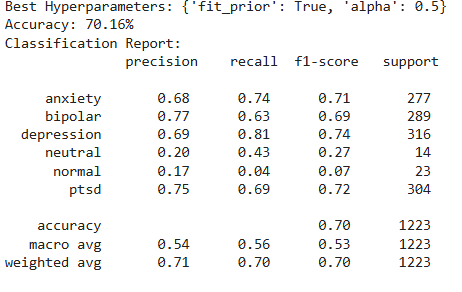
\includegraphics[width=0.8\textwidth]{Images/Output HPT NB.png}  
    \caption{Result of Hyperparameter Tuning on Naive Bayes}
    \label{HPT NB}  % Label for referencing the figure
\end{figure}

\begin{figure}[h!]  
    \centering
    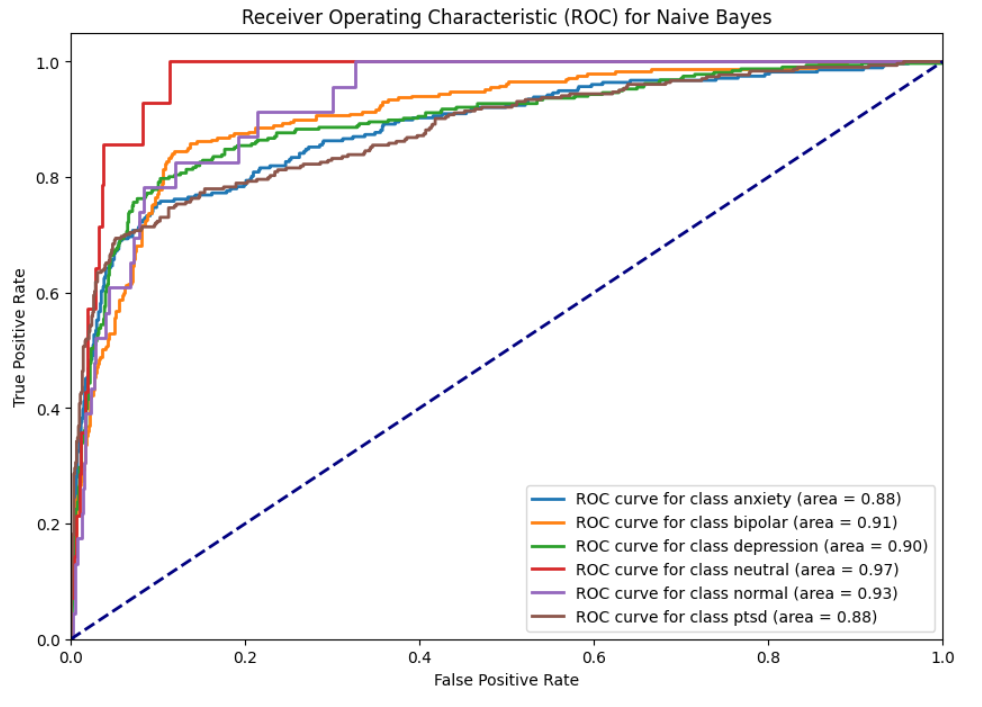
\includegraphics[width=0.8\textwidth]{Images/ROC NB.png}  
    \caption{ROC Curve on Naive bayes}
    \label{ROC NB}  % Label for referencing the figure
\end{figure}

\subssubection{Random Forest}
\noindent
The following code snippet demonstrates the implementation of a Random Forest classifier for classifying mental health issues based on preprocessed text data.

\begin{figure}[h!]  
    \centering
    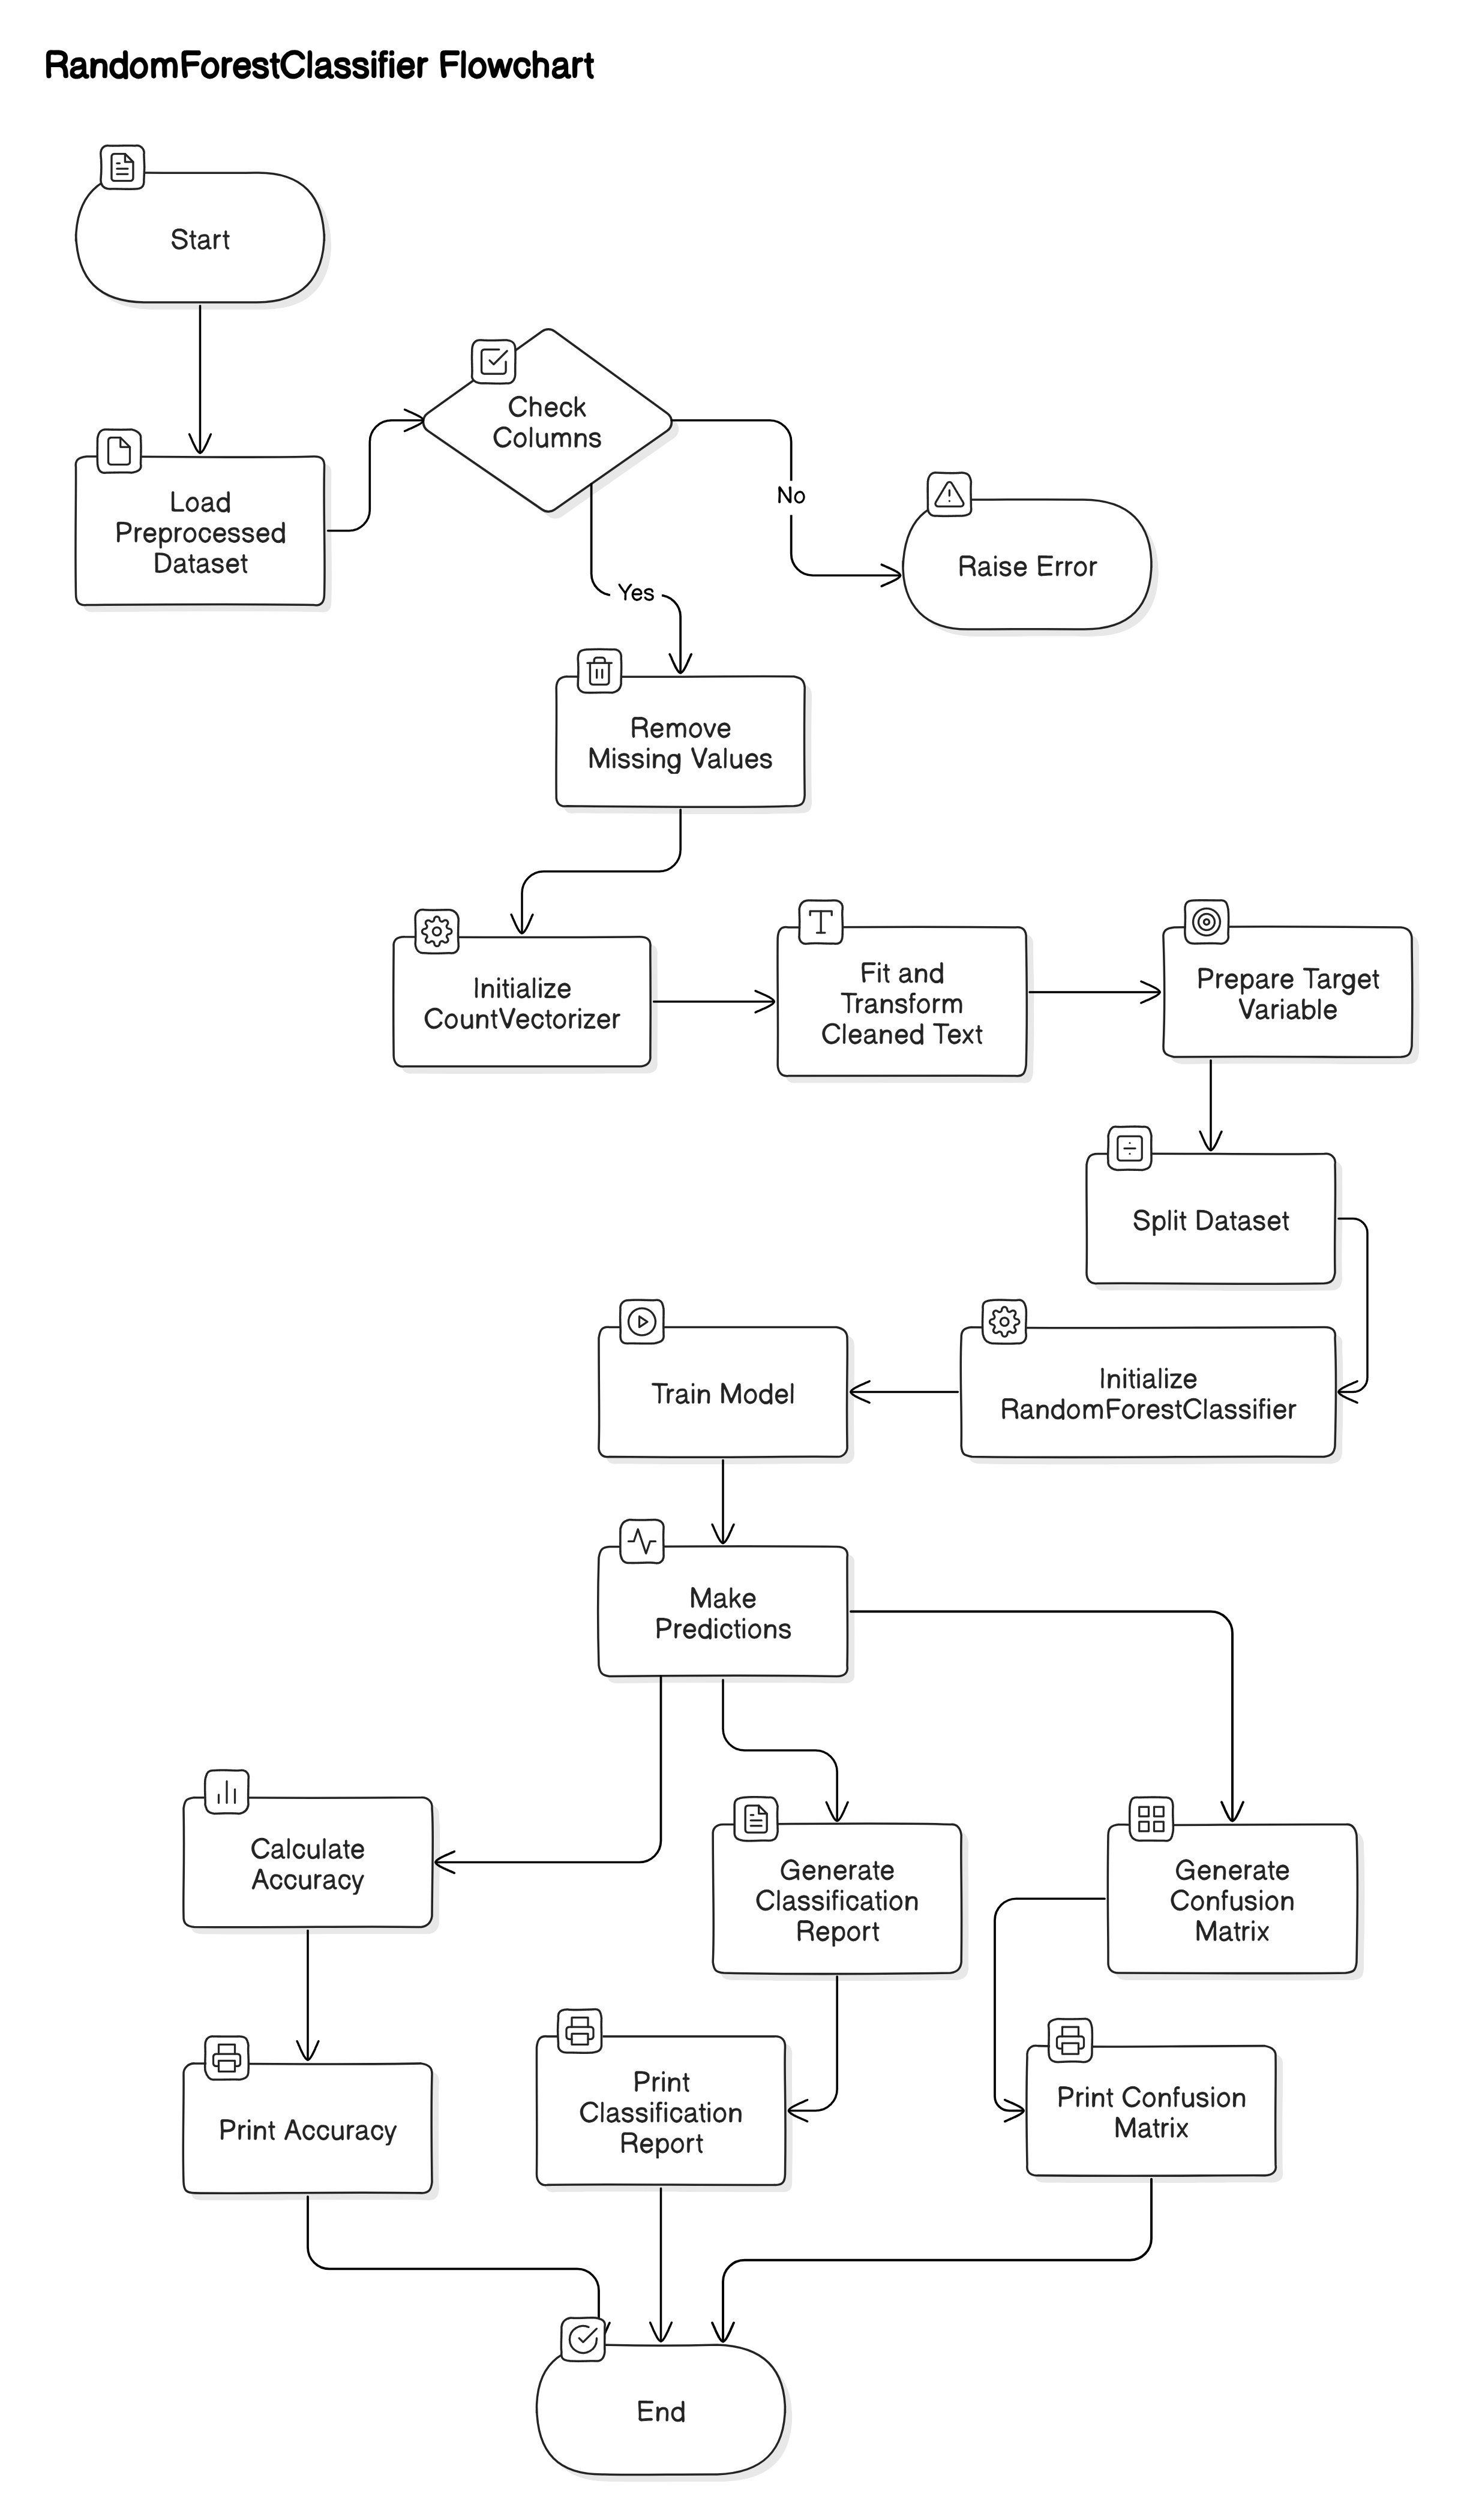
\includegraphics[width=0.6\textwidth]{Images/Random Forest.png}  
    \caption{Random Forest Workflow}
    \label{Random Forest}  % Label for referencing the figure
\end{figure}

\begin{verbatim}
import pandas as pd
from sklearn.model_selection import train_test_split
from sklearn.feature_extraction.text import CountVectorizer
from sklearn.ensemble import RandomForestClassifier
from sklearn.metrics import accuracy_score, classification_report, 
confusion_matrix
dataset = pd.read_csv('preprocessed_mental_health_text.csv')
if 'cleaned_text' not in dataset.columns or 'mental_health_issue' 
not in dataset.columns:
    raise ValueError("The dataset must have 'cleaned_text' and 
    'mental_health_issue' columns.")
dataset.dropna(subset=['cleaned_text'], inplace=True)
vectorizer = CountVectorizer()
X = vectorizer.fit_transform(dataset['cleaned_text'])
y = dataset['mental_health_issue']
X_train, X_test, y_train, y_test = train_test_split(X, y, 
test_size=0.2, random_state=42)
rf_model = RandomForestClassifier(
    n_estimators=3000,
    max_depth=None,
    min_samples_split=20,
    min_samples_leaf=1,
    max_features='sqrt',
    bootstrap=False,
    random_state=42
)
rf_model.fit(X_train, y_train)
y_pred = rf_model.predict(X_test)
accuracy = accuracy_score(y_test, y_pred)
print(f'Accuracy: {accuracy * 100:.2f}%')
print("Classification Report:\n", 
classification_report(y_test, y_pred))
print("Confusion Matrix:\n", confusion_matrix(y_test, y_pred))
\end{verbatim}

\noindent
The code begins by importing the necessary libraries, including \texttt{pandas} for data manipulation and various functions from \texttt{sklearn} for model training and evaluation. It loads the preprocessed dataset from a CSV file named \texttt{preprocessed\_mental\_health\_text.csv} and checks for the presence of the required columns, raising a \texttt{ValueError} if either the \texttt{cleaned\_text} or \texttt{mental\_health\_issue} columns are missing. Rows with missing values in the \texttt{cleaned\_text} column are then removed to ensure data quality. \\

\noindent
The \texttt{CountVectorizer} is initialized to convert the cleaned text into a numerical format, which is stored in \(X\), while the target variable representing mental health issues is assigned to \(y\). The dataset is split into training and testing sets, with 80\% used for training and 20\% for testing. A Random Forest classifier is initialized with specific parameters, including the number of trees (\texttt{n\_estimators}), the minimum number of samples required to split a node (\texttt{min\_samples\_split}), the minimum number of samples in a leaf node (\texttt{min\_samples\_leaf}), and the number of features to consider when looking for the best split (\texttt{max\_features}). The model is then trained using the training data, and predictions are made on the test set. The accuracy of the model is calculated and displayed, along with a classification report and confusion matrix that provide detailed metrics on the model's performance across different categories.

\begin{figure}[h!]  
    \centering
    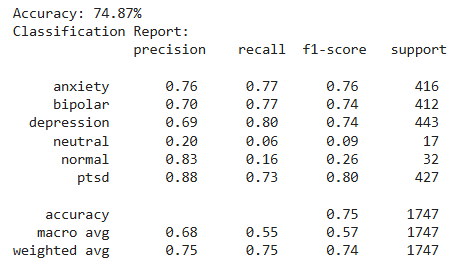
\includegraphics[width=0.9\textwidth]{Images/Output RF.png}  
    \caption{Random Forest Result}
    \label{Random Forest}  % Label for referencing the figure
\end{figure}

\begin{figure}[h!]  
    \centering
    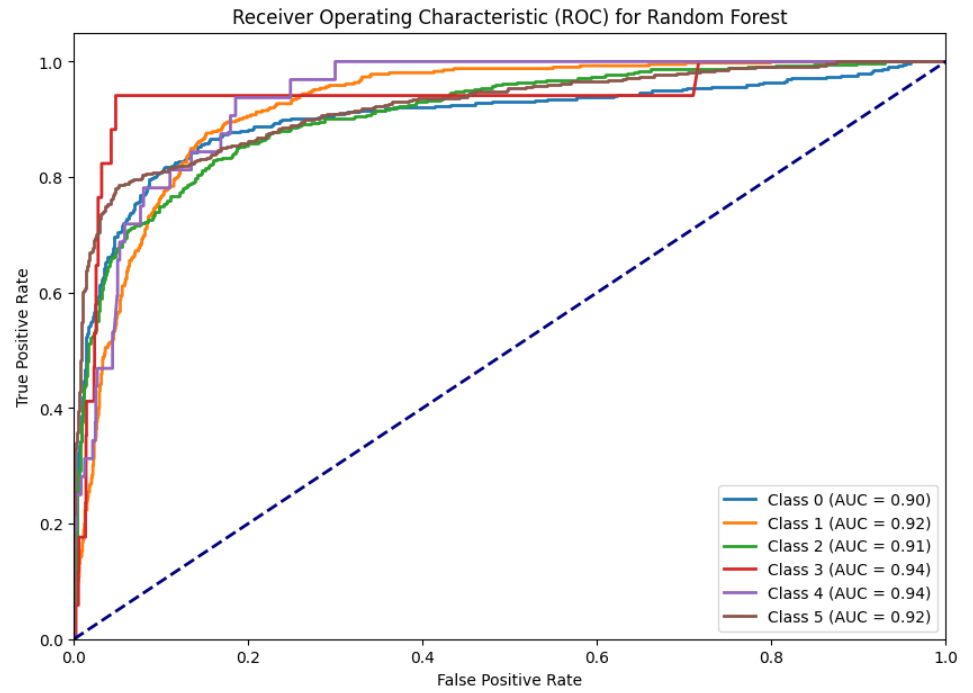
\includegraphics[width=0.9\textwidth]{Images/ROC RF.png}  
    \caption{ROC Curve on Random Forest}
    \label{ROC RF}  % Label for referencing the figure
\end{figure}



% ------------------------- Implementation Ends -----------------------------


% -------------------- Result and Analysis ----------------------------------

\pagebreak

\section{Results and Analysis}
%Prepare the test plans in tabular format, where each Test Case should be represented with distinct id, prefixed with “$\langle$module$\rangle$ “, where module represents the short code of the respective design module. Test Case numbers should be matching as stated in Requirement Matrix.
%\vspace{.1in}

%\noindent

%Appropriate definition of ‘Performance Metrics’, e.g. Classification Accuracy, Mean Squared Error etc. should be included, as applicable. 
%\vspace{.1in}

%\noindent
%Depending on your specific project, test results can be represented as a table of data with a corresponding pie chart / bar chart as needed. Analysis of test results should be discussed in terms of clear bullet points.

\noindent
The metrics used for evaluating the performance of the classification models include Precision, Recall, F1-Score, and Support, along with the Confusion Matrix. These metrics are crucial for assessing how well the models are able to differentiate between various classes, providing insight into their accuracy, ability to capture relevant instances, and the overall balance between precision and recall. By analyzing these metrics, a comprehensive understanding of the model's performance can be obtained, enabling informed decisions for further optimization and tuning.

\subsection{Classification Metrics and Confusion Matrix}

\begin{itemize}
    \item \textbf{Precision:} Precision is the ratio of correctly predicted positive observations to the total predicted positives. It can be calculated as:
    \[
    \text{Precision} = \frac{TP}{TP + FP}
    \]
    where \( TP \) represents True Positives, and \( FP \) represents False Positives.

    \item \textbf{Recall:} Recall is the ratio of correctly predicted positive observations to all observations in the actual class:
    \[
    \text{Recall} = \frac{TP}{TP + FN}
    \]
    where \( TP \) is True Positives, and \( FN \) is False Negatives.

    \item \textbf{F1-Score:} F1-Score is the harmonic mean of Precision and Recall, calculated as:
    \[
    \text{F1-Score} = 2 \times \frac{\text{Precision} \times \text{Recall}}{\text{Precision} + \text{Recall}}
    \]

    \item \textbf{Support:} Support refers to the number of actual occurrences of each class in the dataset:
    \[
    \text{Support} = \text{Number of samples in the true class}
    \]

    \item \textbf{Confusion Matrix:} A confusion matrix is used to evaluate the performance of a classification model. It is structured as follows:
    \[
    \begin{bmatrix}
    TP & FP \\
    FN & TN
    \end{bmatrix}
    \]
    where:
    \begin{itemize}
        \item \( TP \) = True Positives
        \item \( FP \) = False Positives
        \item \( FN \) = False Negatives
        \item \( TN \) = True Negatives
    \end{itemize}
\end{itemize}

\subsection{Results of Logistic Regression and Hyperparameter Tuning}

\begin{center}
    \caption{Logistic Regression Classification Report (Before Hyperparameter Tuning)} \\
\begin{tabular}{|l|c|c|c|c|}
\hline
\textbf{Class} & \textbf{Precision} & \textbf{Recall} & \textbf{F1-Score} & \textbf{Support} \\ \hline
Anxiety        & 0.78               & 0.73            & 0.75              & 416              \\ \hline
Bipolar        & 0.66               & 0.84            & 0.74              & 412              \\ \hline
Depression     & 0.74               & 0.72            & 0.73              & 443              \\ \hline
Neutral        & 0.08               & 0.06            & 0.07              & 17               \\ \hline
Normal         & 0.78               & 0.22            & 0.34              & 32               \\ \hline
PTSD           & 0.83               & 0.74            & 0.78              & 427              \\ \hline
\textbf{Accuracy} & \multicolumn{4}{|c|}{73.78\%} \\ \hline
\textbf{Macro Avg} & 0.64            & 0.55            & 0.57              & 1747             \\ \hline
\textbf{Weighted Avg} & 0.75         & 0.74            & 0.74              & 1747             \\ \hline
\end{tabular} \\

 \vspace{0.25in}% Reduces space between tables

\caption{Logistic Regression Classification Report (After Hyperparameter Tuning)} \\
\begin{tabular}{|l|c|c|c|c|}
\hline
\textbf{Class} & \textbf{Precision} & \textbf{Recall} & \textbf{F1-Score} & \textbf{Support} \\ \hline
Anxiety        & 0.80               & 0.75            & 0.77              & 416              \\ \hline
Bipolar        & 0.66               & 0.85            & 0.74              & 412              \\ \hline
Depression     & 0.75               & 0.74            & 0.75              & 443              \\ \hline
Neutral        & 0.14               & 0.12            & 0.13              & 17               \\ \hline
Normal         & 0.78               & 0.22            & 0.34              & 32               \\ \hline
PTSD           & 0.86               & 0.75            & 0.80              & 427              \\ \hline
\textbf{Accuracy} & \multicolumn{4}{|c|}{75.27\%} \\ \hline
\textbf{Macro Avg} & 0.67            & 0.57            & 0.59              & 1747             \\ \hline
\textbf{Weighted Avg} & 0.76         & 0.75            & 0.75              & 1747             \\ \hline
\end{tabular} \\

  \vspace{0.25in}% Reduces space between tables

\caption{Confusion Matrix for Logistic Regression (After Hyperparameter Tuning)} \\
\begin{tabular}{|l|c|c|c|c|c|c|}
\hline
\textbf{True Class} & \textbf{Anxiety} & \textbf{Bipolar} & \textbf{Depression} & \textbf{Neutral} & \textbf{Normal} & \textbf{PTSD} \\ \hline
Anxiety             & 310              & 45               & 37                  & 2                & 1               & 21            \\ \hline
Bipolar             & 12               & 349              & 35                  & 5                & 1               & 10            \\ \hline
Depression          & 34               & 62               & 327                 & 2                & 0               & 18            \\ \hline
Neutral             & 1                & 8                & 5                   & 2                & 0               & 1             \\ \hline
Normal              & 1                & 23               & 1                   & 0                & 7               & 0             \\ \hline
PTSD                & 31               & 44               & 29                  & 3                & 0               & 320           \\ \hline
\end{tabular}
\end{center}

\subsection{Explanation of the Results (Logistic Regression)}

\textbf{Overall Performance:}

The Logistic Regression model's initial accuracy was \textbf{73.78\%}, which improved to \textbf{75.27\%} after hyperparameter tuning using Randomized Search.

\textbf{Improvement After Hyperparameter Tuning:}

\begin{itemize}
    \item The tuned model showed a slight increase in accuracy, reflecting an improved ability to distinguish between the different mental health classes.
    \item The precision, recall, and F1-scores for most of the individual classes also showed minor improvements.
\end{itemize}

\textbf{Class-wise Analysis:}

\begin{itemize}
    \item \textbf{Anxiety:} The precision and recall improved slightly, indicating better classification of anxiety-related texts.
    \item \textbf{Bipolar:} A notable increase in recall suggests the tuned model became more sensitive to identifying bipolar instances correctly.
    \item \textbf{Depression:} The performance metrics remained relatively stable, showing the model was consistently able to handle depression cases.
    \item \textbf{Neutral \& Normal:} Low precision and recall values indicate that the model struggles to correctly classify these rare classes, likely due to insufficient support (sample size).
\end{itemize}


\begin{figure}[h!]  
    \centering
    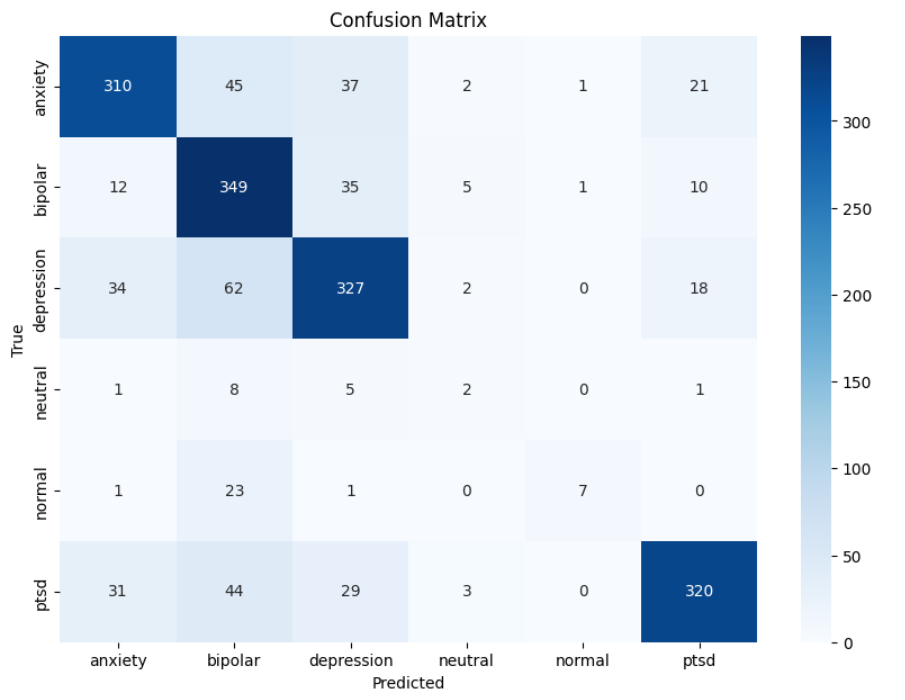
\includegraphics[width=1.0\textwidth]{Images/Confusion Matrix LR.png}  
    \caption{Confusion Matrix for Logistic Regression}
    \label{Project Modules}  % Label for referencing the figure
\end{figure}

\pagebreak
\textbf{Confusion Matrix Analysis:}

\begin{itemize}
    \item The confusion matrix reveals where the model misclassifies different categories. For example:
    \begin{itemize}
        \item \textbf{Anxiety} is often confused with \textbf{Bipolar} and \textbf{Depression}, indicating overlapping features between these classes.
        \item \textbf{PTSD} is more distinct, as shown by a higher number of true positive predictions (320), suggesting that the model can better differentiate this category.
    \end{itemize}
    \item Overall, the confusion matrix helps pinpoint specific classes where the model's predictions are less reliable, providing direction for further improvements.
\end{itemize}




\subsection{Results of K-Nearest Neighbors (KNN) and Hyperparameter Tuning}

\begin{center}
    \caption{KNN Classification Report (Before Hyperparameter Tuning)}
\begin{tabular}{|l|c|c|c|c|}
\hline
\textbf{Class} & \textbf{Precision} & \textbf{Recall} & \textbf{F1-Score} & \textbf{Support} \\ \hline
Anxiety        & 0.60               & 0.36            & 0.45              & 416              \\ \hline
Bipolar        & 0.31               & 0.83            & 0.45              & 412              \\ \hline
Depression     & 0.46               & 0.35            & 0.40              & 443              \\ \hline
Neutral        & 0.00               & 0.00            & 0.00              & 17               \\ \hline
Normal         & 0.29               & 0.06            & 0.10              & 32               \\ \hline
PTSD           & 0.81               & 0.11            & 0.20              & 427              \\ \hline
\textbf{Accuracy} & \multicolumn{4}{|c|}{39.61\%} \\ \hline
\textbf{Macro Avg} & 0.41            & 0.28            & 0.27              & 1747             \\ \hline
\textbf{Weighted Avg} & 0.54         & 0.40            & 0.36              & 1747             \\ \hline
\end{tabular}


\vspace{0.25in}

\caption{Confusion Matrix for KNN (Before Hyperparameter Tuning)}
\begin{tabular}{|l|c|c|c|c|c|c|}
\hline
\textbf{True Class} & \textbf{Anxiety} & \textbf{Bipolar} & \textbf{Depression} & \textbf{Neutral} & \textbf{Normal} & \textbf{PTSD} \\ \hline
Anxiety             & 148              & 221              & 46                  & 0                & 0               & 1             \\ \hline
Bipolar             & 24               & 340              & 42                  & 1                & 3               & 2             \\ \hline
Depression          & 36               & 246              & 154                 & 0                & 0               & 7             \\ \hline
Neutral             & 2                & 14               & 0                   & 0                & 0               & 1             \\ \hline
Normal              & 0                & 30               & 0                   & 0                & 2               & 0             \\ \hline
PTSD                & 38               & 248              & 91                  & 0                & 2               & 48            \\ \hline
\end{tabular}


\vspace{1.5in}

\pagebreak
\caption{KNN Classification Report (After Hyperparameter Tuning)}
\begin{tabular}{|l|c|c|c|c|}
\hline
\textbf{Class} & \textbf{Precision} & \textbf{Recall} & \textbf{F1-Score} & \textbf{Support} \\ \hline
Anxiety        & 0.65               & 0.34            & 0.45              & 416              \\ \hline
Bipolar        & 0.32               & 0.82            & 0.46              & 412              \\ \hline
Depression     & 0.47               & 0.39            & 0.43              & 443              \\ \hline
Neutral        & 0.00               & 0.00            & 0.00              & 17               \\ \hline
Normal         & 0.26               & 0.19            & 0.22              & 32               \\ \hline
PTSD           & 0.73               & 0.15            & 0.24              & 427              \\ \hline
\textbf{Accuracy} & \multicolumn{4}{|c|}{41.27\%} \\ \hline
\textbf{Macro Avg} & 0.40            & 0.31            & 0.30              & 1747             \\ \hline
\textbf{Weighted Avg} & 0.53         & 0.41            & 0.39              & 1747             \\ \hline
\end{tabular}


\vspace{0.25in}

\caption{Confusion Matrix for KNN (After Hyperparameter Tuning)}
\begin{tabular}{|l|c|c|c|c|c|c|}
\hline
\textbf{True Class} & \textbf{Anxiety} & \textbf{Bipolar} & \textbf{Depression} & \textbf{Neutral} & \textbf{Normal} & \textbf{PTSD} \\ \hline
Anxiety             & 143              & 214              & 52                  & 0                & 2               & 5             \\ \hline
Bipolar             & 19               & 337              & 45                  & 1                & 7               & 3             \\ \hline
Depression          & 31               & 223              & 173                 & 1                & 1               & 14            \\ \hline
Neutral             & 0                & 15               & 1                   & 0                & 0               & 1             \\ \hline
Normal              & 0                & 26               & 0                   & 0                & 6               & 0             \\ \hline
PTSD                & 28               & 233              & 97                  & 0                & 7               & 62            \\ \hline
\end{tabular}
\end{center}

\subsection{Explanations for KNN Results}

\begin{itemize}
    \item \textbf{Initial KNN Performance:}
    \begin{itemize}
        \item The initial accuracy of the KNN model is low (\textbf{39.61\%}), indicating that the model struggles to classify the mental health categories effectively.
        \item The recall for the \textbf{Bipolar} class is high (0.83), suggesting that the model is sensitive to detecting bipolar cases but tends to misclassify other categories as bipolar.
        \item Other classes like \textbf{Neutral} and \textbf{Normal} have very low precision and recall, highlighting the model’s inability to distinguish these less frequent categories.
    \end{itemize}

    \item \textbf{After Hyperparameter Tuning:}
    \begin{itemize}
        \item The accuracy improved slightly to \textbf{41.27\%} after tuning with the best hyperparameters \{'weights': 'distance', 'n\_neighbors': 4, 'metric': 'euclidean'\}, indicating minor gains in the classification.
        \item The recall for the \textbf{Anxiety} class decreased, while the precision increased, showing a trade-off in performance.
        \item For the \textbf{Depression} class, both precision and recall increased slightly, indicating that the tuning helped the model distinguish depression cases better.
    \end{itemize}

    \item \textbf{Confusion Matrix Analysis:}
    \begin{itemize}
        \item Many instances of \textbf{Anxiety} and \textbf{Depression} are misclassified as \textbf{Bipolar}, showing overlapping features between these classes.
        \item The class \textbf{PTSD} has a low recall, indicating that most of the PTSD samples are misclassified into other categories.
        \item The class distribution imbalance and similar feature patterns might be contributing to the misclassifications, causing the model to favor more common classes like Bipolar.
    \end{itemize}
\end{itemize}

\begin{figure}[h!]  
    \centering
    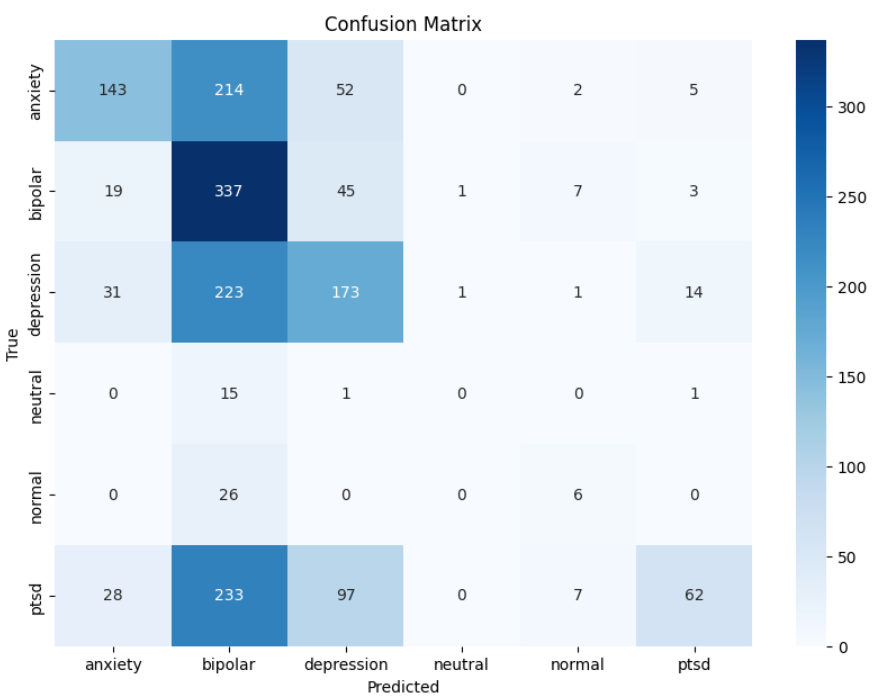
\includegraphics[width=1.0\textwidth]{Images/Confusion Matrix KNN.png}  
    \caption{Confusion Matrix for KNN}
    \label{Confusion Matrix KNN}  % Label for referencing the figure
\end{figure}

\pagebreak
\subsection{Results of Support Vector Machine (SVM) and Hyperparameter Tuning}

\begin{center}
    \caption{SVM Classification Report (Before Hyperparameter Tuning)}
\begin{tabular}{|l|c|c|c|c|}
\hline
\textbf{Class} & \textbf{Precision} & \textbf{Recall} & \textbf{F1-Score} & \textbf{Support} \\ \hline
Anxiety        & 0.70               & 0.70            & 0.70              & 416              \\ \hline
Bipolar        & 0.65               & 0.81            & 0.72              & 412              \\ \hline
Depression     & 0.72               & 0.67            & 0.69              & 443              \\ \hline
Neutral        & 0.19               & 0.18            & 0.18              & 17               \\ \hline
Normal         & 0.62               & 0.25            & 0.36              & 32               \\ \hline
PTSD           & 0.81               & 0.71            & 0.76              & 427              \\ \hline
\textbf{Accuracy} & \multicolumn{4}{|c|}{70.75\%} \\ \hline
\textbf{Macro Avg} & 0.61            & 0.55            & 0.57              & 1747             \\ \hline
\textbf{Weighted Avg} & 0.71         & 0.71            & 0.71              & 1747             \\ \hline
\end{tabular}

\vspace{0.25in}

\caption{Confusion Matrix for SVM (Before Hyperparameter Tuning)}
\begin{tabular}{|l|c|c|c|c|c|c|}
\hline
\textbf{True Class} & \textbf{Anxiety} & \textbf{Bipolar} & \textbf{Depression} & \textbf{Neutral} & \textbf{Normal} & \textbf{PTSD} \\ \hline
Anxiety             & 292              & 45               & 44                  & 2                & 1               & 32            \\ \hline
Bipolar             & 23               & 333              & 37                  & 5                & 3               & 11            \\ \hline
Depression          & 59               & 58               & 296                 & 2                & 0               & 28            \\ \hline
Neutral             & 1                & 7                & 5                   & 3                & 0               & 1             \\ \hline
Normal              & 0                & 24               & 0                   & 0                & 8               & 0             \\ \hline
PTSD                & 41               & 47               & 30                  & 4                & 1               & 304           \\ \hline
\end{tabular}

\vspace{0.25in}

\caption{SVM Classification Report (After Hyperparameter Tuning)}
\begin{tabular}{|l|c|c|c|c|}
\hline
\textbf{Class} & \textbf{Precision} & \textbf{Recall} & \textbf{F1-Score} & \textbf{Support} \\ \hline
Anxiety        & 0.78               & 0.71            & 0.74              & 416              \\ \hline
Bipolar        & 0.61               & 0.83            & 0.70              & 412              \\ \hline
Depression     & 0.75               & 0.70            & 0.72              & 443              \\ \hline
Neutral        & 0.13               & 0.12            & 0.12              & 17               \\ \hline
Normal         & 0.57               & 0.12            & 0.21              & 32               \\ \hline
PTSD           & 0.84               & 0.71            & 0.77              & 427              \\ \hline
\textbf{Accuracy} & \multicolumn{4}{|c|}{72.07\%} \\ \hline
\textbf{Macro Avg} & 0.61            & 0.53            & 0.54              & 1747             \\ \hline
\textbf{Weighted Avg} & 0.73         & 0.72            & 0.72              & 1747             \\ \hline
\end{tabular}

\vspace{0.25in}

\caption{Confusion Matrix for SVM (After Hyperparameter Tuning)}
\begin{tabular}{|l|c|c|c|c|c|c|}
\hline
\textbf{True Class} & \textbf{Anxiety} & \textbf{Bipolar} & \textbf{Depression} & \textbf{Neutral} & \textbf{Normal} & \textbf{PTSD} \\ \hline
Anxiety             & 292              & 45               & 44                  & 2                & 1               & 32            \\ \hline
Bipolar             & 23               & 333              & 37                  & 5                & 3               & 11            \\ \hline
Depression          & 59               & 58               & 296                 & 2                & 0               & 28            \\ \hline
Neutral             & 1                & 7                & 5                   & 3                & 0               & 1             \\ \hline
Normal              & 0                & 24               & 0                   & 0                & 8               & 0             \\ \hline
PTSD                & 41               & 47               & 30                  & 4                & 1               & 304           \\ \hline
\end{tabular}
\end{center}

\subsection{Explanations for SVM Results}

\begin{itemize}
    \item \textbf{Initial SVM Performance:}
    \begin{itemize}
        \item The initial accuracy of the SVM model is \textbf{70.75\%}, indicating a moderate performance in classifying mental health categories.
        \item The \textbf{Bipolar} class has a high recall of 0.81, indicating the model's ability to identify most bipolar cases correctly. However, the precision is lower, showing misclassification with other classes.
        \item The \textbf{Neutral} and \textbf{Normal} classes have low precision and recall values, indicating that the model struggles to identify these minority classes.
    \end{itemize}

    \item \textbf{After Hyperparameter Tuning:}
    \begin{itemize}
        \item The accuracy improved slightly to \textbf{72.07\%} with the best hyperparameters \{'kernel': 'linear', 'gamma': 'scale', 'C': 0.1\}.
        \item The recall for the \textbf{Anxiety} and \textbf{Depression} classes increased, indicating better sensitivity to these categories.
        \item The precision for \textbf{PTSD} also improved, suggesting the model has a clearer distinction for this class after tuning.
    \end{itemize}

    \begin{figure}[h!]  
    \centering
    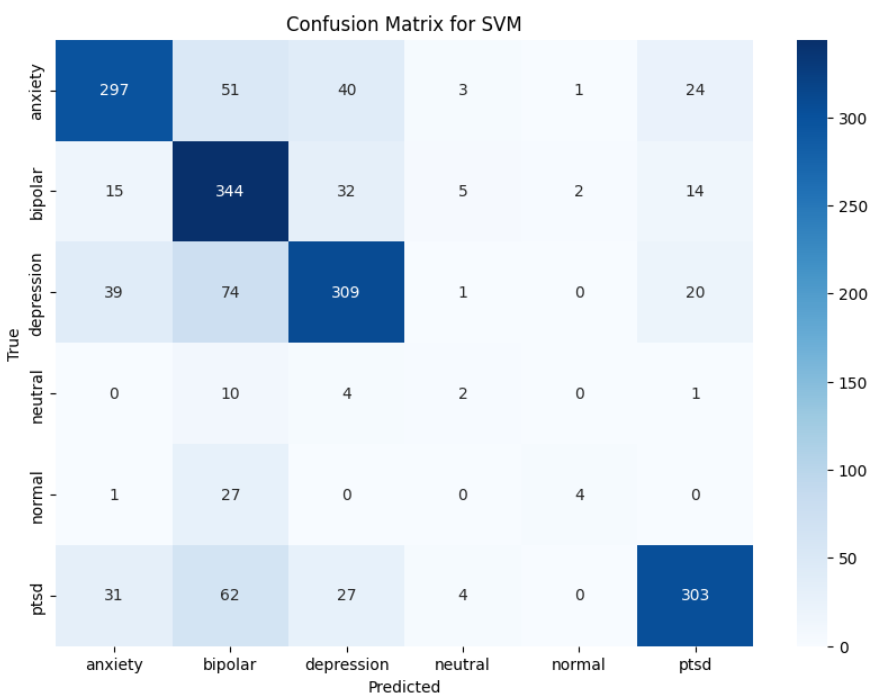
\includegraphics[width=0.8\textwidth]{Images/Confusion Matrix SVM.png}  
    \caption{Confusion Matrix for SVM}
    \label{Confusion Matrix SVM}  % Label for referencing the figure
    \end{figure}

    \item \textbf{Confusion Matrix Analysis:}
    \begin{itemize}
        \item Many instances of \textbf{Anxiety} and \textbf{Depression} are misclassified as \textbf{Bipolar}, showing overlapping features between these classes.
        \item The \textbf{Neutral} and \textbf{Normal} classes have very few true positive predictions, indicating that the SVM model still struggles to capture these less frequent categories.
        \item Overall, the slight improvement in performance after hyperparameter tuning suggests that tuning helped the SVM classifier better balance the trade-offs between precision and recall for most major classes.
    \end{itemize}
\end{itemize}



\subsection{Results of Naive Bayes and Hyperparameter Tuning}

\begin{center}
    \caption{Naive Bayes Classification Report (Before Hyperparameter Tuning)}
\begin{tabular}{|l|c|c|c|c|}
\hline
\textbf{Class} & \textbf{Precision} & \textbf{Recall} & \textbf{F1-Score} & \textbf{Support} \\ \hline
Anxiety        & 0.69               & 0.72            & 0.70              & 416              \\ \hline
Bipolar        & 0.79               & 0.56            & 0.65              & 412              \\ \hline
Depression     & 0.65               & 0.82            & 0.72              & 443              \\ \hline
Neutral        & 0.17               & 0.29            & 0.21              & 17               \\ \hline
Normal         & 0.14               & 0.03            & 0.05              & 32               \\ \hline
PTSD           & 0.73               & 0.72            & 0.72              & 427              \\ \hline
\textbf{Accuracy} & \multicolumn{4}{|c|}{68.92\%} \\ \hline
\textbf{Macro Avg} & 0.53            & 0.52            & 0.51              & 1747             \\ \hline
\textbf{Weighted Avg} & 0.70         & 0.69            & 0.68              & 1747             \\ \hline
\end{tabular}

\vspace{0.25in}

\caption{Confusion Matrix for Naive Bayes (Before Hyperparameter Tuning)}
\begin{tabular}{|l|c|c|c|c|c|c|}
\hline
\textbf{True Class} & \textbf{Anxiety} & \textbf{Bipolar} & \textbf{Depression} & \textbf{Neutral} & \textbf{Normal} & \textbf{PTSD} \\ \hline
Anxiety             & 300              & 14               & 61                  & 8                & 3               & 30            \\ \hline
Bipolar             & 51               & 229              & 78                  & 5                & 0               & 49            \\ \hline
Depression          & 27               & 20               & 362                 & 5                & 1               & 28            \\ \hline
Neutral             & 1                & 6                & 4                   & 5                & 1               & 0             \\ \hline
Normal              & 12               & 2                & 9                   & 1                & 1               & 7             \\ \hline
PTSD                & 46               & 20               & 47                  & 6                & 1               & 307           \\ \hline
\end{tabular}

\vspace{0.25in}

\caption{Naive Bayes Classification Report (After Hyperparameter Tuning)}
\begin{tabular}{|l|c|c|c|c|}
\hline
\textbf{Class} & \textbf{Precision} & \textbf{Recall} & \textbf{F1-Score} & \textbf{Support} \\ \hline
Anxiety        & 0.68               & 0.74            & 0.71              & 277              \\ \hline
Bipolar        & 0.77               & 0.63            & 0.69              & 289              \\ \hline
Depression     & 0.69               & 0.81            & 0.74              & 316              \\ \hline
Neutral        & 0.20               & 0.43            & 0.27              & 14               \\ \hline
Normal         & 0.17               & 0.04            & 0.07              & 23               \\ \hline
PTSD           & 0.75               & 0.69            & 0.72              & 304              \\ \hline
\textbf{Accuracy} & \multicolumn{4}{|c|}{70.16\%} \\ \hline
\textbf{Macro Avg} & 0.54            & 0.56            & 0.53              & 1223             \\ \hline
\textbf{Weighted Avg} & 0.71         & 0.70            & 0.70              & 1223             \\ \hline
\end{tabular}

\vspace{0.25in}

\caption{Confusion Matrix for Naive Bayes (After Hyperparameter Tuning)}
\begin{tabular}{|l|c|c|c|c|c|c|}
\hline
\textbf{True Class} & \textbf{Anxiety} & \textbf{Bipolar} & \textbf{Depression} & \textbf{Neutral} & \textbf{Normal} & \textbf{PTSD} \\ \hline
Anxiety             & 300              & 14               & 61                  & 8                & 3               & 30            \\ \hline
Bipolar             & 51               & 229              & 78                  & 5                & 0               & 49            \\ \hline
Depression          & 27               & 20               & 362                 & 5                & 1               & 28            \\ \hline
Neutral             & 1                & 6                & 4                   & 5                & 1               & 0             \\ \hline
Normal              & 12               & 2                & 9                   & 1                & 1               & 7             \\ \hline
PTSD                & 46               & 20               & 47                  & 6                & 1               & 307           \\ \hline
\end{tabular}    
\end{center}

\subsection{Explanations for Naive Bayes Results}

\begin{itemize}
    \item \textbf{Initial Naive Bayes Performance:}
    \begin{itemize}
        \item The initial accuracy of the Naive Bayes model is \textbf{68.92\%}, indicating moderate classification performance.
        \item The \textbf{Anxiety} and \textbf{Depression} classes have relatively higher recall values, suggesting that the model is sensitive to identifying these categories correctly.
        \item The \textbf{Neutral} and \textbf{Normal} classes have very low precision and recall, indicating that the model struggles to classify these minority classes.
    \end{itemize}

    \item \textbf{After Hyperparameter Tuning:}
    \begin{itemize}
        \item The accuracy increased slightly to \textbf{70.16\%} with the best hyperparameters \{'fit\_prior': True, 'alpha': 0.5\}, showing a minor performance improvement.
        \item The recall for the \textbf{Anxiety} and \textbf{Depression} classes increased, indicating better sensitivity and improved classification for these classes.
        \item However, the precision for the \textbf{Bipolar} class decreased slightly, suggesting a trade-off in correctly identifying true positive cases for this class.
    \end{itemize}
    
    \item \textbf{Confusion Matrix Analysis:}
    \begin{itemize}
        \item Many instances of \textbf{Anxiety} and \textbf{Depression} are misclassified as \textbf{Bipolar}, indicating overlapping feature characteristics between these categories.
        \item The \textbf{Neutral} and \textbf{Normal} classes continue to have very few true positive predictions, highlighting the model’s struggle to capture these less frequent categories.
        \item The increase in recall for major classes like \textbf{Anxiety} and \textbf{Depression} after tuning suggests that the model learned better class-specific distributions.
    \end{itemize}
\end{itemize}

 \begin{figure}[h!]  
    \centering
    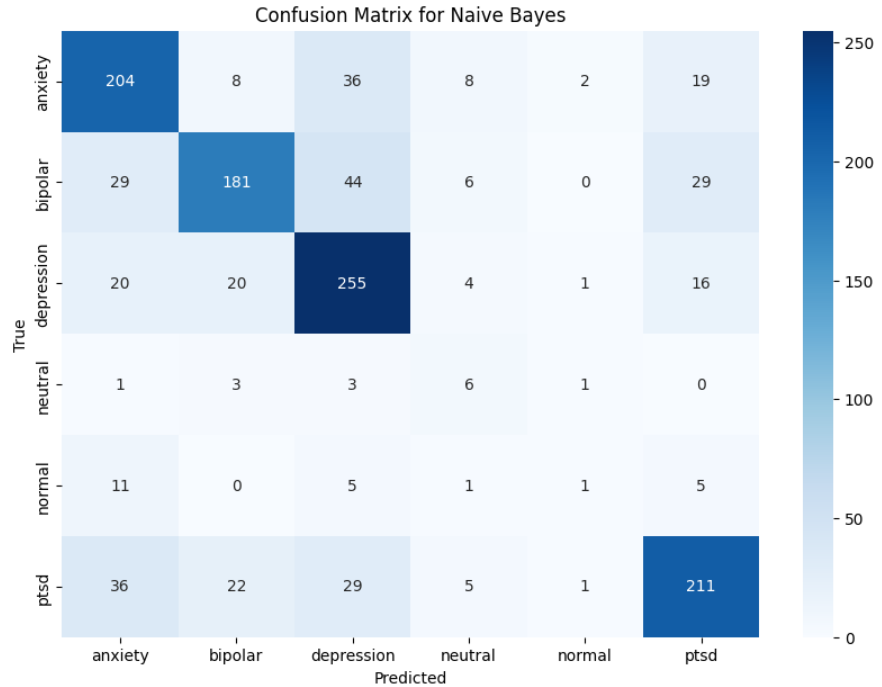
\includegraphics[width=0.8\textwidth]{Images/Confusion Matrix NB.png}  
    \caption{Confusion Matrix for Naive Bayes}
    \label{Confusion Matrix NB}  % Label for referencing the figure
    \end{figure}

\subsection{Results of Random Forest and Hyperparameter Tuning}

\begin{center}
    \caption{Random Forest Classification Report}
\begin{tabular}{|l|c|c|c|c|}
\hline
\textbf{Class} & \textbf{Precision} & \textbf{Recall} & \textbf{F1-Score} & \textbf{Support} \\ \hline
Anxiety        & 0.76               & 0.77            & 0.76              & 416              \\ \hline
Bipolar        & 0.70               & 0.77            & 0.74              & 412              \\ \hline
Depression     & 0.69               & 0.80            & 0.74              & 443              \\ \hline
Neutral        & 0.20               & 0.06            & 0.09              & 17               \\ \hline
Normal         & 0.83               & 0.16            & 0.26              & 32               \\ \hline
PTSD           & 0.88               & 0.73            & 0.80              & 427              \\ \hline
\textbf{Accuracy} & \multicolumn{4}{|c|}{74.87\%} \\ \hline
\textbf{Macro Avg} & 0.68            & 0.55            & 0.57              & 1747             \\ \hline
\textbf{Weighted Avg} & 0.75         & 0.75            & 0.74              & 1747             \\ \hline
\end{tabular}

\vspace{0.25in}

\caption{Confusion Matrix for Random Forest}
\begin{tabular}{|l|c|c|c|c|c|c|}
\hline
\textbf{True Class} & \textbf{Anxiety} & \textbf{Bipolar} & \textbf{Depression} & \textbf{Neutral} & \textbf{Normal} & \textbf{PTSD} \\ \hline
Anxiety             & 319              & 38               & 50                  & 0                & 0               & 9             \\ \hline
Bipolar             & 23               & 319              & 53                  & 2                & 1               & 14            \\ \hline
Depression          & 31               & 41               & 353                 & 0                & 0               & 18            \\ \hline
Neutral             & 1                & 9                & 5                   & 1                & 0               & 1             \\ \hline
Normal              & 3                & 24               & 0                   & 0                & 5               & 0             \\ \hline
PTSD                & 43               & 22               & 49                  & 2                & 0               & 311           \\ \hline
\end{tabular}    
\end{center}

\subsection{Explanations for Random Forest Results}

\begin{itemize}
    \item \textbf{Overall Performance:}
    \begin{itemize}
        \item The accuracy of the Random Forest model is \textbf{74.87\%}, indicating a good level of performance in classifying the different mental health categories.
        \item The \textbf{PTSD} class shows the highest precision (0.88) and recall (0.73), suggesting that the model is effective at identifying PTSD cases correctly.
    \end{itemize}

    \item \textbf{Class-wise Analysis:}
    \begin{itemize}
        \item The precision and recall for the \textbf{Anxiety} and \textbf{Depression} classes are reasonably balanced, indicating that the model is adept at classifying these categories.
        \item The \textbf{Bipolar} class has a slightly lower precision but high recall, suggesting that while the model can identify bipolar instances effectively, it also misclassifies some non-bipolar cases as bipolar.
        \item The performance for the \textbf{Neutral} and \textbf{Normal} classes is concerning, with very low recall and F1-scores, indicating that these classes are often misclassified.
    \end{itemize}

    \begin{figure}[h!]  
    \centering
    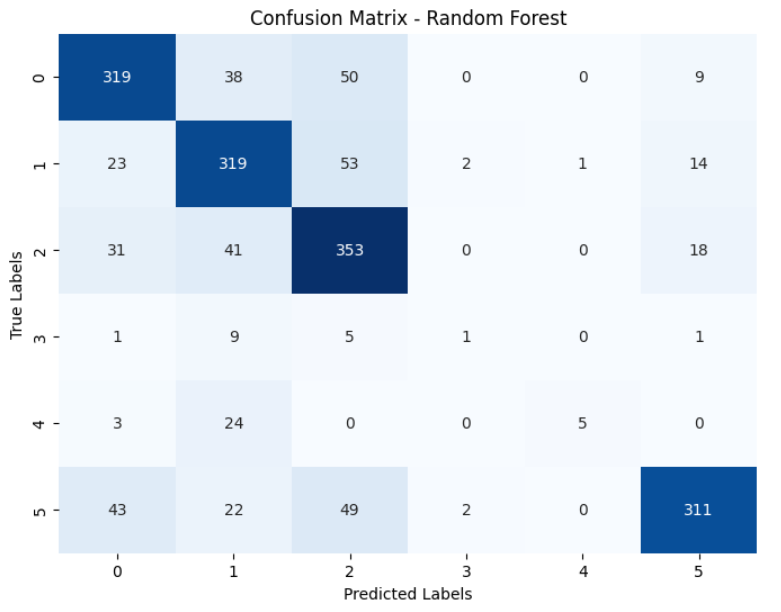
\includegraphics[width=0.9\textwidth]{Images/Confusion Matrix RF.png}  
    \caption{Confusion Matrix for Random Forest}
    \label{Confusion Matrix RF}  % Label for referencing the figure
    \end{figure}

    \item \textbf{Confusion Matrix Analysis:}
    \begin{itemize}
        \item The confusion matrix reveals that many instances of \textbf{Anxiety} and \textbf{Depression} are correctly classified, with a significant number of \textbf{Neutral} instances being misclassified.
        \item The low count for \textbf{Normal} indicates that the model has trouble distinguishing this category, as evidenced by the high number of false positives.
        \item The high number of true positive predictions for \textbf{PTSD} (311) suggests that the Random Forest model is effective in distinguishing PTSD from other classes, likely due to its ability to handle complex feature interactions well.
    \end{itemize}
\end{itemize}

\subsection{Comparison of Different Models}

\begin{center}
    \centering
    \caption{Datasets Overview} \\
    \vspace{0.05in}
    \begin{tabular}{|l|c|c|c|}
    \hline
    \textbf{Dataset} & \textbf{Capacity} & \textbf{Modality} \\ \hline
    Dataset - Reddit  & 12000              & Single            \\ \hline
    Dataset - Twitter  & 900                & Single            \\ \hline
    DS - Reddit + Twitter & 12900          & Single            \\ \hline
    \end{tabular}

    \vspace{0.25in}

\centering
\caption{Comparison of Classification Metrics for Anxiety}
\begin{tabular}{|l|c|c|c|c|}
\hline
\textbf{Model} & \textbf{Precision} & \textbf{Recall} & \textbf{F1-Score} & \textbf{Support} \\ \hline
Logistic Regression & 0.78 & 0.73 & 0.75 & 416 \\ \hline
KNN                & 0.60 & 0.36 & 0.45 & 416 \\ \hline
SVM                & 0.70 & 0.70 & 0.70 & 416 \\ \hline
Naive Bayes        & 0.69 & 0.72 & 0.70 & 416 \\ \hline
Random Forest      & 0.76 & 0.77 & 0.76 & 416 \\ \hline
\end{tabular}

\vspace{0.25in}

\centering
\caption{Comparison of Classification Metrics for Bipolar}
\begin{tabular}{|l|c|c|c|c|}
\hline
\textbf{Model} & \textbf{Precision} & \textbf{Recall} & \textbf{F1-Score} & \textbf{Support} \\ \hline
Logistic Regression & 0.66 & 0.84 & 0.74 & 412 \\ \hline
KNN                & 0.31 & 0.83 & 0.45 & 412 \\ \hline
SVM                & 0.65 & 0.81 & 0.72 & 412 \\ \hline
Naive Bayes        & 0.79 & 0.56 & 0.65 & 412 \\ \hline
Random Forest      & 0.70 & 0.77 & 0.74 & 412 \\ \hline
\end{tabular}

\vspace{0.25in}

\centering
\caption{Comparison of Classification Metrics for Depression}
\begin{tabular}{|l|c|c|c|c|}
\hline
\textbf{Model} & \textbf{Precision} & \textbf{Recall} & \textbf{F1-Score} & \textbf{Support} \\ \hline
Logistic Regression & 0.74 & 0.72 & 0.73 & 443 \\ \hline
KNN                & 0.46 & 0.35 & 0.40 & 443 \\ \hline
SVM                & 0.72 & 0.67 & 0.69 & 443 \\ \hline
Naive Bayes        & 0.65 & 0.82 & 0.72 & 443 \\ \hline
Random Forest      & 0.69 & 0.80 & 0.74 & 443 \\ \hline
\end{tabular}

\vspace{0.25in}

\centering
\caption{Comparison of Classification Metrics for Neutral}
\begin{tabular}{|l|c|c|c|c|}
\hline
\textbf{Model} & \textbf{Precision} & \textbf{Recall} & \textbf{F1-Score} & \textbf{Support} \\ \hline
Logistic Regression & 0.08 & 0.06 & 0.07 & 17 \\ \hline
KNN                & 0.00 & 0.00 & 0.00 & 17 \\ \hline
SVM                & 0.19 & 0.18 & 0.18 & 17 \\ \hline
Naive Bayes        & 0.17 & 0.29 & 0.21 & 17 \\ \hline
Random Forest      & 0.20 & 0.06 & 0.09 & 17 \\ \hline
\end{tabular}


\vspace{0.25in}

\caption{Comparison of Classification Metrics for Normal}
\begin{tabular}{|l|c|c|c|c|}
\hline
\textbf{Model} & \textbf{Precision} & \textbf{Recall} & \textbf{F1-Score} & \textbf{Support} \\ \hline
Logistic Regression & 0.78 & 0.22 & 0.34 & 32 \\ \hline
KNN                & 0.29 & 0.06 & 0.10 & 32 \\ \hline
SVM                & 0.62 & 0.25 & 0.36 & 32 \\ \hline
Naive Bayes        & 0.14 & 0.03 & 0.05 & 32 \\ \hline
Random Forest      & 0.83 & 0.16 & 0.26 & 32 \\ \hline
\end{tabular}

\vspace{0.25in}

\caption{Comparison of Classification Metrics for PTSD}
\begin{tabular}{|l|c|c|c|c|}
\hline
\textbf{Model} & \textbf{Precision} & \textbf{Recall} & \textbf{F1-Score} & \textbf{Support} \\ \hline
Logistic Regression & 0.83 & 0.74 & 0.78 & 427 \\ \hline
KNN                & 0.81 & 0.11 & 0.20 & 427 \\ \hline
SVM                & 0.81 & 0.71 & 0.76 & 427 \\ \hline
Naive Bayes        & 0.73 & 0.72 & 0.72 & 427 \\ \hline
Random Forest      & 0.88 & 0.73 & 0.80 & 427 \\ \hline
\end{tabular}

\vspace{0.25in}

\caption{Comparison of Classification Metrics for Anxiety (After Hyperparameter Tuning)}
\begin{tabular}{|l|c|c|c|c|}
\hline
\textbf{Model} & \textbf{Precision} & \textbf{Recall} & \textbf{F1-Score} & \textbf{Support} \\ \hline
Logistic Regression & 0.80 & 0.75 & 0.77 & 416 \\ \hline
KNN                & 0.65 & 0.34 & 0.45 & 416 \\ \hline
SVM                & 0.78 & 0.71 & 0.74 & 416 \\ \hline
Naive Bayes        & 0.68 & 0.74 & 0.71 & 277 \\ \hline
\end{tabular}

\vspace{0.25in}

\caption{Comparison of Classification Metrics for Bipolar (After Hyperparameter Tuning)}
\begin{tabular}{|l|c|c|c|c|}
\hline
\textbf{Model} & \textbf{Precision} & \textbf{Recall} & \textbf{F1-Score} & \textbf{Support} \\ \hline
Logistic Regression & 0.66 & 0.85 & 0.74 & 412 \\ \hline
KNN                & 0.32 & 0.82 & 0.46 & 412 \\ \hline
SVM                & 0.61 & 0.83 & 0.70 & 412 \\ \hline
Naive Bayes        & 0.77 & 0.63 & 0.69 & 289 \\ \hline
\end{tabular}

\vspace{0.25in}

\caption{Comparison of Classification Metrics for Depression (After Hyperparameter Tuning)}
\begin{tabular}{|l|c|c|c|c|}
\hline
\textbf{Model} & \textbf{Precision} & \textbf{Recall} & \textbf{F1-Score} & \textbf{Support} \\ \hline
Logistic Regression & 0.75 & 0.74 & 0.75 & 443 \\ \hline
KNN                & 0.47 & 0.39 & 0.43 & 443 \\ \hline
SVM                & 0.75 & 0.70 & 0.72 & 443 \\ \hline
Naive Bayes        & 0.69 & 0.81 & 0.74 & 316 \\ \hline
\end{tabular}

\vspace{0.25in}

\caption{Comparison of Classification Metrics for Neutral (After Hyperparameter Tuning)}
\begin{tabular}{|l|c|c|c|c|}
\hline
\textbf{Model} & \textbf{Precision} & \textbf{Recall} & \textbf{F1-Score} & \textbf{Support} \\ \hline
Logistic Regression & 0.14 & 0.12 & 0.13 & 17 \\ \hline
KNN                & 0.00 & 0.00 & 0.00 & 17 \\ \hline
SVM                & 0.13 & 0.12 & 0.12 & 17 \\ \hline
Naive Bayes        & 0.20 & 0.43 & 0.27 & 14 \\ \hline
\end{tabular}

\vspace{0.25in}

\caption{Comparison of Classification Metrics for Normal (After Hyperparameter Tuning)}
\begin{tabular}{|l|c|c|c|c|}
\hline
\textbf{Model} & \textbf{Precision} & \textbf{Recall} & \textbf{F1-Score} & \textbf{Support} \\ \hline
Logistic Regression & 0.78 & 0.22 & 0.34 & 32 \\ \hline
KNN                & 0.26 & 0.19 & 0.22 & 32 \\ \hline
SVM                & 0.57 & 0.12 & 0.21 & 32 \\ \hline
Naive Bayes        & 0.17 & 0.04 & 0.07 & 23 \\ \hline
\end{tabular}

\vspace{0.25in}

\caption{Comparison of Classification Metrics for PTSD (After Hyperparameter Tuning)}
\begin{tabular}{|l|c|c|c|c|}
\hline
\textbf{Model} & \textbf{Precision} & \textbf{Recall} & \textbf{F1-Score} & \textbf{Support} \\ \hline
Logistic Regression & 0.86 & 0.75 & 0.80 & 427 \\ \hline
KNN                & 0.73 & 0.15 & 0.24 & 427 \\ \hline
SVM                & 0.84 & 0.71 & 0.77 & 427 \\ \hline
Naive Bayes        & 0.75 & 0.69 & 0.72 & 304 \\ \hline
\end{tabular}

\end{center}


% ------------------------ Result and Analysis Ends -------------------------



% ------------------------------ Conclusion ---------------------------------

\section{Conclusion}
% State the project benefits. Outline the future scope for improvements.

\subsection{Project Benefits}
\noindent
The project on detecting mental health disorders through social media analysis offers a wide array of significant benefits, both immediate and long-term, across multiple dimensions. First and foremost, it addresses a critical issue in mental health care—early detection and intervention. Social media has become a ubiquitous platform where people express their thoughts, feelings, and emotional states, often unconsciously. By leveraging the vast amounts of data available on social media platforms, our project seeks to tap into this resource to identify early signs of mental health disorders such as anxiety, depression, and more severe conditions like bipolar disorder or schizophrenia. The ability to detect mental health issues through real-time social media data is a game-changer for public health systems, mental health practitioners, and even individuals who may not realize they are at risk. Early detection enables timely intervention, reducing the overall burden of mental health disorders on society by preventing escalation into more severe conditions that often lead to hospitalization, self-harm, or even suicide. In this sense, the project aligns with global health initiatives that emphasize early diagnosis and preventive care. \\

\noindent
Moreover, this project holds significant potential for improving the accuracy and efficiency of mental health diagnostics. Traditional diagnostic methods are often time-consuming, subjective, and reliant on self-reporting, which can lead to underdiagnosis or misdiagnosis. By utilizing machine learning algorithms and natural language processing techniques, our project automates the process of sentiment and behavioral analysis on social media platforms, offering a more objective and data-driven approach. This automated system can process large volumes of data much faster than human professionals, providing insights that would be impossible to glean from manual analysis. The algorithms developed as part of this project can be easily scaled to analyze millions of social media posts, enabling a broader reach in monitoring public mental health trends. Additionally, the project offers practical benefits for mental health professionals, allowing them to focus on treatment and intervention rather than diagnosis. It provides a tool that can be integrated into telehealth systems, offering mental health screening at scale, which is particularly valuable in underserved or rural areas where access to mental health professionals is limited. \\

\noindent
From a technological standpoint, the project offers a host of reusable components and methodologies. The machine learning models developed, the sentiment analysis tools, and the overall data pipeline are designed to be scalable and modular. These components can be adapted and extended to other domains beyond mental health, such as market sentiment analysis, public opinion monitoring, or even detecting harmful behavior like cyberbullying and harassment online. By advancing the state of the art in social media analytics, this project contributes to the growing field of AI-driven health care solutions. Furthermore, it provides a blueprint for future interdisciplinary work that integrates data science, psychology, and public health. \\

\subsection{Future Scope for Improvements}
\noindent
While this project offers numerous immediate benefits, there is substantial room for future enhancements that can broaden its applicability, accuracy, and effectiveness. One of the key areas for improvement lies in the expansion of data sources. Currently, the project focuses on analyzing Twitter sentiment data from Kaggle, which is limited to a specific social media platform and dataset. In the future, incorporating data from other platforms like Facebook, Instagram, Reddit, and even niche forums could provide a more comprehensive understanding of an individual’s mental health status. Different platforms cater to different demographics and social behaviors, and expanding the dataset will allow for a more holistic analysis of mental health indicators across various user bases. Additionally, expanding the dataset to include multilingual posts or integrating language translation capabilities could make the system applicable to a global audience, helping to identify mental health issues in non-English speaking populations. \\

\noindent
Another area ripe for future development is the improvement of the machine learning models used for mental health prediction. Current models, while effective, could benefit from more advanced techniques such as deep learning architectures, which are particularly powerful in handling unstructured data like text and images. For instance, implementing models like transformers or neural networks that can better understand the context and nuance in human language could lead to more accurate predictions. Additionally, incorporating multi-modal data, such as analyzing images and videos along with textual data, could provide richer insights into a user’s mental health state. Emotions and mental health issues are often expressed visually as well, and combining these different data types could significantly improve the system’s accuracy. \\

\noindent
Moreover, future improvements could focus on integrating real-time data analysis capabilities. Currently, our project is based on batch processing of historical data. However, in future iterations, the system could be developed to perform real-time monitoring, offering immediate feedback and potentially alerting health professionals or loved ones when someone shows signs of mental distress. This real-time capability would be invaluable in emergency situations, allowing for immediate intervention. Developing a mobile application or a web-based interface where users can voluntarily connect their social media accounts to monitor their mental health status could also increase user engagement and provide individuals with direct feedback on their well-being. \\

\noindent
Another significant future enhancement could involve incorporating ethical considerations and improving user privacy. As mental health is a sensitive subject, ensuring that the system is designed with robust privacy protections is critical. Future work could focus on using differential privacy or other anonymization techniques to ensure that user data remains confidential while still allowing for effective analysis. Moreover, collaborating with psychologists, ethicists, and legal experts could help refine the system to ensure it adheres to ethical guidelines and avoids potential harm, such as misdiagnosis or privacy violations. \\

\noindent
Lastly, the future scope of this project could include expanding its use in clinical settings. While the current system is primarily designed as a research tool, future iterations could be developed in collaboration with mental health professionals to ensure that it meets clinical standards. By integrating this system with electronic health records or telehealth platforms, it could become a critical tool in mental health care, helping practitioners monitor their patients’ mental health between sessions. This would allow for a more proactive approach to mental health care, potentially reducing the need for emergency interventions and improving overall treatment outcomes.

% ------------------------- Conclusion Ends ----------------------------------



% --------------------------------- References ------------------------------
 \pagebreak

\section{References}

\begin{comment}
    Please list all referred papers / articles / journals / books including your own published papers / patent (if applicable). Listing and citations should follow IEEE standard format.
    
\end{comment}

\vspace{-6em}
\noindent
\renewcommand{\refname}{} % Removes the References title that appears by default
\bibliographystyle{plain}
\bibliography{references}

% -------------------------------- References End ----------------------------





\begin{comment}
    \section{APPENDIX A - Prototypes (optional) \label{sec:proto}}
Provide the filtered part of RM showing selected features for prototype building. State the detailed steps of compilation, execution and setups. Specify prototype details showing codes, screens, test data, sample output and detailed steps of compilation, execution and setups (if any).


    \section{APPENDIX B - Paper publications (optional) \label{sec:pubs}}
If any of your related paper(s) were published in a standard journal / presented in a recognized conference, mention the same including communication on your paper(s) acceptance / publishing note. You should also show appropriate documentation at the time of project viva.
    
\end{comment}



 %\section*{APPENDIX A - Prototypes (optional) \label{sec:proto}}
\addcontentsline{toc}{section}{APPENDIX A - Prototypes (optional)}
Provide the filtered part of RM showing selected features for prototype building. State the detailed steps of compilation, execution and setups. Specify prototype details showing codes, screens, test data, sample output and detailed steps of compilation, execution and setups (if any).

\section*{APPENDIX B - Paper publications (optional) \label{sec:pubs}}
\addcontentsline{toc}{section}{APPENDIX B - Paper publications (optional)}
If any of your related paper(s) were published in a standard journal / presented in a recognized conference, mention the same including communication on your paper(s) acceptance / publishing note. You should also show appropriate documentation at the time of project viva.
% \addcontentsline{toc}{section}{Bibliography}
%\bibliographystyle{IEEEtran}
%\bibliography{references}
 
%TODO: remove the following after your report is completed
% by commenting the next line
%%\thispagestyle{plain}
\color{red}
{\large \bf \underline {Instructions (remove these after completing your report ):}}
%\subsection{Edit and generate pdf}
\color{black}
\begin{enumerate}[label=\roman*.]
\item 	Double-click in the page header and replace “Project Name” text with your short project name.

\item \textcolor{blue} {
{If you have an external guide, ensure to insert (Signature of External Guide) at the left of (Signature of the External Examiner) on the APPROVAL page.}} If inserted, ensure to align the second line with the first line.

\item Insert \textbf{Appendix section(s)} at the end of this document if you need to elaborate any specific item, e.g. Data Collection if it is taking too many pages to cover.

\item 	\textcolor{blue}{\textbf{At the time of final examination, 1 spiral-bound project report should be submitted to the department in addition to the soft copy deliverables}}.

\item Citations should be used for all referred texts using appropriate numbers within square bracket for all mapped references under \textbf{References} section. You should check any standard journal paper for typical use of citations. 

\item 	Select Content (TOC), and apply Font Size=12. After completing the document, ensure to right-click on ToC $\rightarrow$ Update field  $\rightarrow$ Update entire table for automatically updating the index. If needed, change the font or adjust headings so that TOC can be fitted in a single page.

\item	Except under TOC, \textbf{Font} Style=”Times New Roman”, Font Size=”12” and Alignment=”Justified” should be uniformly used for the project documentation. Needless to say \textbf{spellchecker} should be used. 

\item Team should perform reasonable numbers of \textbf{proof reading} for avoiding unintentional errors and factual discrepancies before appearing in project viva.

\item	For all \textbf{ figures}, captions should be bold with centrally aligned and should be positioned below the figures, e.g.

Using MS-Word features, insert figures and tables after they are cited in the text so that they can automatically come after inserting / updating TOC.	 

Use a text box to insert a graphic (which is ideally a 300 dpi TIFF or EPS file, with all fonts embedded) because, in an MS Word document, this method is somewhat more stable than directly inserting a picture.

To have non-visible rules on your frame, use the MSWord “Format” pull-down menu, select Text Box $>$ Colors and Lines to choose No Fill and No Line.

\item For all \textbf{tables}, captions should be bold with centrally aligned and should be positioned above the tables, e.g.
\begin{figure}[h]  % Optional: figure environment to allow caption and positioning
    \centering      % Center the image
    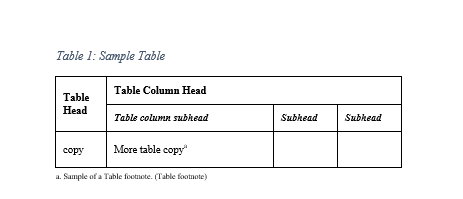
\includegraphics[width=\textwidth]{Table} % Specify the image file name
    %\caption{A caption for the image.}  % Optional: add a caption
    \label{fig:example}  % Optional: label for referencing the image
\end{figure}


\item	Based on your unique project, sections can be slightly altered over this generic template.

\end{enumerate}
\begin{comment}
    

\begin{enumerate}
\item You need to create an account in overleaf \url{https://www.overleaf.com/project} (if not already created) and login.
\item Select `New project' $\rightarrow$ `Upload project'  $\rightarrow$ select `LaTex\_template\_BTP\_Report.zip' file.
You need to do this step only once.
Next time on-wards, you can directly access the folder in overleaf and make necessary changes.
\item Only one person from the group can upload the project and the share the link to other members of the group who can edit and view the report.
\item Once the folder is loaded, select `BTP\_report.tex' file and click the `Recompile' option. On the right window, you can see the generated pdf where the {\LaTeX} source code is available on the left window.
\item In the `BTP\_report.tex' file change
\begin{itemize}
    \item Project title 
    \item Supervisor name
    \item Supervisor designation 
    \item Name of the HOD
    \item Designation of the HOD 
\item Names and roll numbers of the students
\end{itemize}
\item `Recompile' again to check if the changes are reflected.
\item The PDF file can also be downloaded.
\end{enumerate}
%%\subsection{Adding citations, tables, figures, equations}
\begin{description}
\item \textbf{Equations:}
Basic equations can be written using  Inline math modes such as
\begin{itemize}
    \item using \verb|\(...\)|: \verb|\(x^2 + y^2 = z^2\)| will generate \(x^2 + y^2 = z^2\)
    \item using \texttt{\$...\$}:  \verb|$(x^2 + y^2 = z^2)$| will generate  $(x^2 + y^2 = z^2)$
    \item or, using \verb|\begin{math}...\end{math}|: \\ \verb|\begin{math} x^2 + y^2 = z^2 \end{math}| will generate   \begin{math}(x^2 + y^2 = z^2)\end{math}
\end{itemize}
You can use \verb|\begin{equation}...\end{equation}| for display modes such as 
\verb|\begin{equation} x^2 + y^2 = z^2 \end{equation}| resulting to
\begin{equation} x^2 + y^2 = z^2 \end{equation}
Other details such as adding subscript, superscript, fractions, you can refer to \url{https://www.overleaf.com/learn/latex/Mathematical_expressions}
\item \textbf{Citations:} The citations should be made through adding a `BibTex' entry in `references.bib' file.
Check the examples below:
\begin{verbatim}
  @Article{Einstein,
  author =       "Albert Einstein",
  title =        "{Zur Elektrodynamik bewegter K{\"o}rper}. ({German})
                 [{On} the electrodynamics of moving bodies]",
  journal =      "Annalen der Physik",
  volume =       "322",
  number =       "10",
  pages =        "891--921",
  year =         "1905",
  DOI =          "http://dx.doi.org/10.1002/andp.19053221004"
} 
@online{WinNT,
  author = {MultiMedia LLC},
  title = {{MS Windows NT} Kernel Description},
  year = 1999,
  url = {http://web.archive.org/web/20080207010024},
  urldate = {2010-09-30}
}

@book{knuth1984texbook,
  title={The texbook},
  author={Knuth, Donald Ervin and Bibby, Duane},
  volume={15},
  year={1984},
  publisher={Addison-Wesley Reading}
}  
\end{verbatim}

    % Reference to text book of Donald Knuth \cite{knuth_texboo k}.
\url{https://www.overleaf.com/learn/latex/Bibliography_management_with_bibtex}
Template entries for `BibTex' types of article, conference, book, thesis can be found here \url{https://www.bibtex.com/format/#templates}

The formatted `BibTex' entries of a reference material can also be found in Google Scholar. Search with the title of the paper/thesis/book in Google scholar $\rightarrow$ Select `Cite' option at the bottom the search results $\rightarrow$ Select `Bibtex' option and copy the entry in `references.bib' file.
    


For more detailed examples refer to \url{https://www.overleaf.com/learn/latex/Tables}

\end{description}
{\bf Important}
\begin{enumerate}
\item \textcolor{red}{Remove (Signature of External Guide, if applicable) on the \textbf{CERTIFICATE} page if you don't have an external guide. In any case, \textbf{(Signature of the External Examiner) must be right aligned} as in the template.}
  \item For avoiding plagiarism, citations should be used for all referred texts using appropriate numbers within square bracket for all mapped references under Section 8: References. You should check any standard journal paper for typical use of citations. 

  \item  \textcolor{red}{\textbf{Change the page header and replace “Project Name” text with your short project name}}.


    \item Select the document class 12pt. 

\item Team should perform reasonable numbers of proof reading for avoiding unintentional errors and factual discrepancies before appearing in project viva.


\item  At the time of final examination, (n+1) hard-bound copies of the report requiring (n+1) letter heads should be submitted, where n = team-size and 1 copy should be reserved for the department (not applicable for Midterm or Checkpoint Review)

\item For all figures, captions should be bold with centrally aligned and should be positioned below the figures, e.g.
All image files are to be stored in the Images folder.
For all figures, captions should be bold with centrally aligned and should be
positioned below the figures.
One such example is shown below:
\begin{verbatim}
  \begin{figure}[ht]
    \centering
    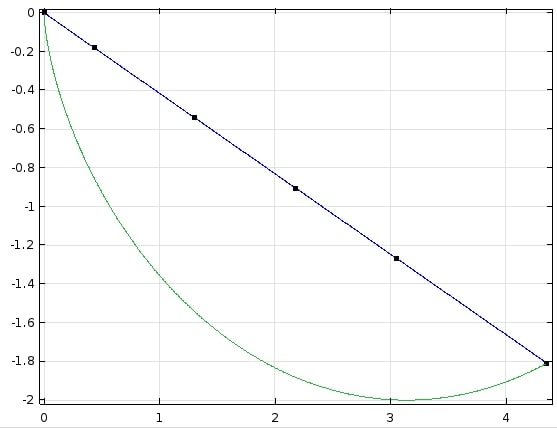
\includegraphics[width=0.5\textwidth]{Brachistochrone-curve-plot.jpg}
    \caption{Sample Image}
    \label{fig:1a}
\end{figure}  
\end{verbatim}
\begin{figure}[ht]
    \centering
    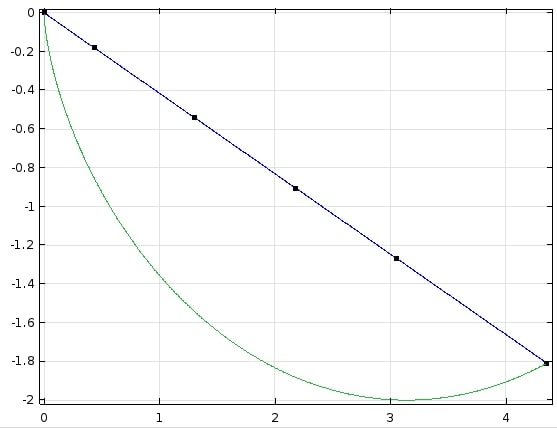
\includegraphics[width=0.5\textwidth]{Brachistochrone-curve-plot.jpg}
    \caption{Sample Image}
    \label{fig:1a}
\end{figure}
This figure will be referenced in the text as Figure \ref{fig:1a}.
For more detailed references for adding figures, refer to \url{https://www.overleaf.com/learn/latex/Inserting_Images}.

\item 
For all tables, captions should be bold with centrally aligned and should be positioned above the tables.
One such example is shown here. 
\begin{verbatim}
\begin{table}[h!]
  \begin{center}
    \caption{Your first table with 3 columns and 5 rows}
    \label{tab:table1}
    
    \begin{tabular}{|c|r|l|} % <-- Alignments: 1st column middle, 
    % 2nd right and 3rd left, 
    % with vertical lines in between each column and row
    % \\
    \hline
      \textbf{Value 1} & \textbf{Value 2} & \textbf{Value 3}\\
      $\alpha$ & $\beta$ & $\gamma$ \\
      \hline
      1 & 1110.1 & a\\
      2 & 10.1 & b\\
      3 & 23.113231 & c\\
      \hline
    \end{tabular}
  \end{center}
\end{table}
\end{verbatim}
\begin{table}[h!]
  \begin{center}
    \caption{Your first table with 3 columns and 5 rows}
    \label{tab:table1}
    
    \begin{tabular}{|c|r|l|} % <-- Alignments: 1st column middle, 2nd right and 3rd left, with vertical lines in between each column and row
    % \\
    \hline
      \textbf{Value 1} & \textbf{Value 2} & \textbf{Value 3}\\
      $\alpha$ & $\beta$ & $\gamma$ \\
      \hline
      1 & 1110.1 & a\\
      2 & 10.1 & b\\
      3 & 23.113231 & c\\
      \hline
    \end{tabular}
  \end{center}
\end{table}

This table can be referenced in the text as Table \ref{tab:table1}.

For more detailed examples refer to \url{https://www.overleaf.com/learn/latex/Tables}

\item If you have published related paper(s) in a standard journal / presented in a recognized conference, please ensure to refer the same under Section 8: References as well as including communication on your paper(s) acceptance / publishing note under the Appendix section. You should also show appropriate documentation at the time of project viva.
\item Depending on the type of your project, sections can be altered to this generic template.



\end{enumerate}

\end{comment}


 % Comment Out 
% \thispagestyle{plain}
\color{red}
{\large \bf \underline {Instructions (remove these after completing your report ):}}
%\subsection{Edit and generate pdf}
\color{black}
\begin{enumerate}[label=\roman*.]
\item 	Double-click in the page header and replace “Project Name” text with your short project name.

\item \textcolor{blue} {
{If you have an external guide, ensure to insert (Signature of External Guide) at the left of (Signature of the External Examiner) on the APPROVAL page.}} If inserted, ensure to align the second line with the first line.

\item Insert \textbf{Appendix section(s)} at the end of this document if you need to elaborate any specific item, e.g. Data Collection if it is taking too many pages to cover.

\item 	\textcolor{blue}{\textbf{At the time of final examination, 1 spiral-bound project report should be submitted to the department in addition to the soft copy deliverables}}.

\item Citations should be used for all referred texts using appropriate numbers within square bracket for all mapped references under \textbf{References} section. You should check any standard journal paper for typical use of citations. 

\item 	Select Content (TOC), and apply Font Size=12. After completing the document, ensure to right-click on ToC $\rightarrow$ Update field  $\rightarrow$ Update entire table for automatically updating the index. If needed, change the font or adjust headings so that TOC can be fitted in a single page.

\item	Except under TOC, \textbf{Font} Style=”Times New Roman”, Font Size=”12” and Alignment=”Justified” should be uniformly used for the project documentation. Needless to say \textbf{spellchecker} should be used. 

\item Team should perform reasonable numbers of \textbf{proof reading} for avoiding unintentional errors and factual discrepancies before appearing in project viva.

\item	For all \textbf{ figures}, captions should be bold with centrally aligned and should be positioned below the figures, e.g.

Using MS-Word features, insert figures and tables after they are cited in the text so that they can automatically come after inserting / updating TOC.	 

Use a text box to insert a graphic (which is ideally a 300 dpi TIFF or EPS file, with all fonts embedded) because, in an MS Word document, this method is somewhat more stable than directly inserting a picture.

To have non-visible rules on your frame, use the MSWord “Format” pull-down menu, select Text Box $>$ Colors and Lines to choose No Fill and No Line.

\item For all \textbf{tables}, captions should be bold with centrally aligned and should be positioned above the tables, e.g.
\begin{figure}[h]  % Optional: figure environment to allow caption and positioning
    \centering      % Center the image
    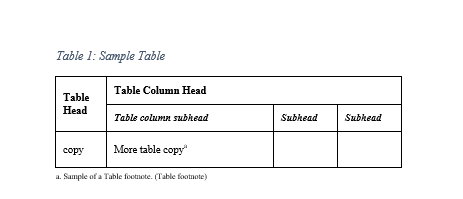
\includegraphics[width=\textwidth]{Table} % Specify the image file name
    %\caption{A caption for the image.}  % Optional: add a caption
    \label{fig:example}  % Optional: label for referencing the image
\end{figure}


\item	Based on your unique project, sections can be slightly altered over this generic template.

\end{enumerate}
\begin{comment}
    

\begin{enumerate}
\item You need to create an account in overleaf \url{https://www.overleaf.com/project} (if not already created) and login.
\item Select `New project' $\rightarrow$ `Upload project'  $\rightarrow$ select `LaTex\_template\_BTP\_Report.zip' file.
You need to do this step only once.
Next time on-wards, you can directly access the folder in overleaf and make necessary changes.
\item Only one person from the group can upload the project and the share the link to other members of the group who can edit and view the report.
\item Once the folder is loaded, select `BTP\_report.tex' file and click the `Recompile' option. On the right window, you can see the generated pdf where the {\LaTeX} source code is available on the left window.
\item In the `BTP\_report.tex' file change
\begin{itemize}
    \item Project title 
    \item Supervisor name
    \item Supervisor designation 
    \item Name of the HOD
    \item Designation of the HOD 
\item Names and roll numbers of the students
\end{itemize}
\item `Recompile' again to check if the changes are reflected.
\item The PDF file can also be downloaded.
\end{enumerate}
%%\subsection{Adding citations, tables, figures, equations}
\begin{description}
\item \textbf{Equations:}
Basic equations can be written using  Inline math modes such as
\begin{itemize}
    \item using \verb|\(...\)|: \verb|\(x^2 + y^2 = z^2\)| will generate \(x^2 + y^2 = z^2\)
    \item using \texttt{\$...\$}:  \verb|$(x^2 + y^2 = z^2)$| will generate  $(x^2 + y^2 = z^2)$
    \item or, using \verb|\begin{math}...\end{math}|: \\ \verb|\begin{math} x^2 + y^2 = z^2 \end{math}| will generate   \begin{math}(x^2 + y^2 = z^2)\end{math}
\end{itemize}
You can use \verb|\begin{equation}...\end{equation}| for display modes such as 
\verb|\begin{equation} x^2 + y^2 = z^2 \end{equation}| resulting to
\begin{equation} x^2 + y^2 = z^2 \end{equation}
Other details such as adding subscript, superscript, fractions, you can refer to \url{https://www.overleaf.com/learn/latex/Mathematical_expressions}
\item \textbf{Citations:} The citations should be made through adding a `BibTex' entry in `references.bib' file.
Check the examples below:
\begin{verbatim}
  @Article{Einstein,
  author =       "Albert Einstein",
  title =        "{Zur Elektrodynamik bewegter K{\"o}rper}. ({German})
                 [{On} the electrodynamics of moving bodies]",
  journal =      "Annalen der Physik",
  volume =       "322",
  number =       "10",
  pages =        "891--921",
  year =         "1905",
  DOI =          "http://dx.doi.org/10.1002/andp.19053221004"
} 
@online{WinNT,
  author = {MultiMedia LLC},
  title = {{MS Windows NT} Kernel Description},
  year = 1999,
  url = {http://web.archive.org/web/20080207010024},
  urldate = {2010-09-30}
}

@book{knuth1984texbook,
  title={The texbook},
  author={Knuth, Donald Ervin and Bibby, Duane},
  volume={15},
  year={1984},
  publisher={Addison-Wesley Reading}
}  
\end{verbatim}

    % Reference to text book of Donald Knuth \cite{knuth_texboo k}.
\url{https://www.overleaf.com/learn/latex/Bibliography_management_with_bibtex}
Template entries for `BibTex' types of article, conference, book, thesis can be found here \url{https://www.bibtex.com/format/#templates}

The formatted `BibTex' entries of a reference material can also be found in Google Scholar. Search with the title of the paper/thesis/book in Google scholar $\rightarrow$ Select `Cite' option at the bottom the search results $\rightarrow$ Select `Bibtex' option and copy the entry in `references.bib' file.
    


For more detailed examples refer to \url{https://www.overleaf.com/learn/latex/Tables}

\end{description}
{\bf Important}
\begin{enumerate}
\item \textcolor{red}{Remove (Signature of External Guide, if applicable) on the \textbf{CERTIFICATE} page if you don't have an external guide. In any case, \textbf{(Signature of the External Examiner) must be right aligned} as in the template.}
  \item For avoiding plagiarism, citations should be used for all referred texts using appropriate numbers within square bracket for all mapped references under Section 8: References. You should check any standard journal paper for typical use of citations. 

  \item  \textcolor{red}{\textbf{Change the page header and replace “Project Name” text with your short project name}}.


    \item Select the document class 12pt. 

\item Team should perform reasonable numbers of proof reading for avoiding unintentional errors and factual discrepancies before appearing in project viva.


\item  At the time of final examination, (n+1) hard-bound copies of the report requiring (n+1) letter heads should be submitted, where n = team-size and 1 copy should be reserved for the department (not applicable for Midterm or Checkpoint Review)

\item For all figures, captions should be bold with centrally aligned and should be positioned below the figures, e.g.
All image files are to be stored in the Images folder.
For all figures, captions should be bold with centrally aligned and should be
positioned below the figures.
One such example is shown below:
\begin{verbatim}
  \begin{figure}[ht]
    \centering
    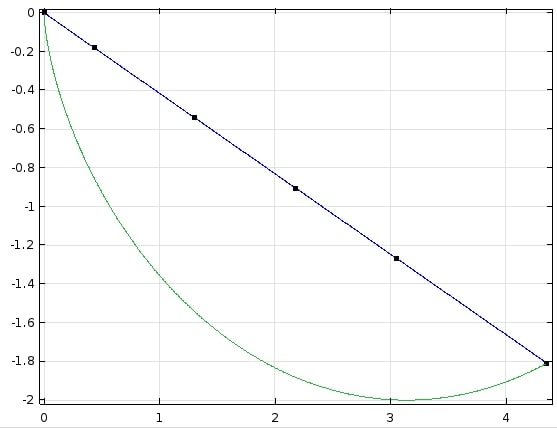
\includegraphics[width=0.5\textwidth]{Brachistochrone-curve-plot.jpg}
    \caption{Sample Image}
    \label{fig:1a}
\end{figure}  
\end{verbatim}
\begin{figure}[ht]
    \centering
    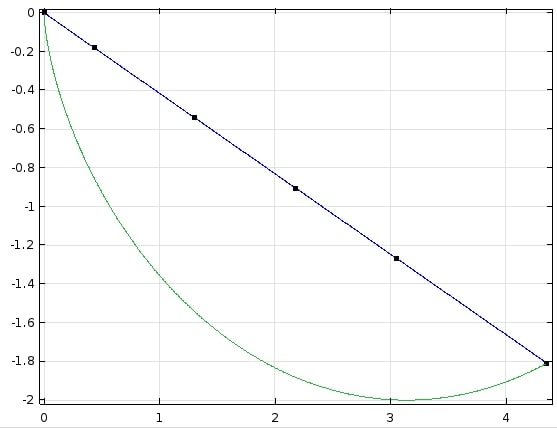
\includegraphics[width=0.5\textwidth]{Brachistochrone-curve-plot.jpg}
    \caption{Sample Image}
    \label{fig:1a}
\end{figure}
This figure will be referenced in the text as Figure \ref{fig:1a}.
For more detailed references for adding figures, refer to \url{https://www.overleaf.com/learn/latex/Inserting_Images}.

\item 
For all tables, captions should be bold with centrally aligned and should be positioned above the tables.
One such example is shown here. 
\begin{verbatim}
\begin{table}[h!]
  \begin{center}
    \caption{Your first table with 3 columns and 5 rows}
    \label{tab:table1}
    
    \begin{tabular}{|c|r|l|} % <-- Alignments: 1st column middle, 
    % 2nd right and 3rd left, 
    % with vertical lines in between each column and row
    % \\
    \hline
      \textbf{Value 1} & \textbf{Value 2} & \textbf{Value 3}\\
      $\alpha$ & $\beta$ & $\gamma$ \\
      \hline
      1 & 1110.1 & a\\
      2 & 10.1 & b\\
      3 & 23.113231 & c\\
      \hline
    \end{tabular}
  \end{center}
\end{table}
\end{verbatim}
\begin{table}[h!]
  \begin{center}
    \caption{Your first table with 3 columns and 5 rows}
    \label{tab:table1}
    
    \begin{tabular}{|c|r|l|} % <-- Alignments: 1st column middle, 2nd right and 3rd left, with vertical lines in between each column and row
    % \\
    \hline
      \textbf{Value 1} & \textbf{Value 2} & \textbf{Value 3}\\
      $\alpha$ & $\beta$ & $\gamma$ \\
      \hline
      1 & 1110.1 & a\\
      2 & 10.1 & b\\
      3 & 23.113231 & c\\
      \hline
    \end{tabular}
  \end{center}
\end{table}

This table can be referenced in the text as Table \ref{tab:table1}.

For more detailed examples refer to \url{https://www.overleaf.com/learn/latex/Tables}

\item If you have published related paper(s) in a standard journal / presented in a recognized conference, please ensure to refer the same under Section 8: References as well as including communication on your paper(s) acceptance / publishing note under the Appendix section. You should also show appropriate documentation at the time of project viva.
\item Depending on the type of your project, sections can be altered to this generic template.



\end{enumerate}

\end{comment}
 
 
 
 %Bibliography

%  \begin{thebibliography}{9}
% \bibitem{knuth_texbook}
% Donald E. Knuth (1986) \emph{The \TeX{} Book}, Addison-Wesley Professional.

% \bibitem{lamport94}
% Leslie Lamport (1994) \emph{\LaTeX: a document preparation system}, Addison
% Wesley, Massachusetts, 2nd ed.
% \end{thebibliography}
 

% \include{./Chapters/9_app1}
% \include{./Chapters/10_app2}
 
\end{document}